\documentclass[twoside]{book}

% Packages required by doxygen
\usepackage{fixltx2e}
\usepackage{calc}
\usepackage{doxygen}
\usepackage[export]{adjustbox} % also loads graphicx
\usepackage{graphicx}
\usepackage[utf8]{inputenc}
\usepackage{makeidx}
\usepackage{multicol}
\usepackage{multirow}
\PassOptionsToPackage{warn}{textcomp}
\usepackage{textcomp}
\usepackage[nointegrals]{wasysym}
\usepackage[table]{xcolor}

% NLS support packages
\usepackage[french]{babel}

% Font selection
\usepackage[T1]{fontenc}
\usepackage[scaled=.90]{helvet}
\usepackage{courier}
\usepackage{amssymb}
\usepackage{sectsty}
\renewcommand{\familydefault}{\sfdefault}
\allsectionsfont{%
  \fontseries{bc}\selectfont%
  \color{darkgray}%
}
\renewcommand{\DoxyLabelFont}{%
  \fontseries{bc}\selectfont%
  \color{darkgray}%
}
\newcommand{\+}{\discretionary{\mbox{\scriptsize$\hookleftarrow$}}{}{}}

% Page & text layout
\usepackage{geometry}
\geometry{%
  a4paper,%
  top=2.5cm,%
  bottom=2.5cm,%
  left=2.5cm,%
  right=2.5cm%
}
\tolerance=750
\hfuzz=15pt
\hbadness=750
\setlength{\emergencystretch}{15pt}
\setlength{\parindent}{0cm}
\setlength{\parskip}{3ex plus 2ex minus 2ex}
\makeatletter
\renewcommand{\paragraph}{%
  \@startsection{paragraph}{4}{0ex}{-1.0ex}{1.0ex}{%
    \normalfont\normalsize\bfseries\SS@parafont%
  }%
}
\renewcommand{\subparagraph}{%
  \@startsection{subparagraph}{5}{0ex}{-1.0ex}{1.0ex}{%
    \normalfont\normalsize\bfseries\SS@subparafont%
  }%
}
\makeatother

% Headers & footers
\usepackage{fancyhdr}
\pagestyle{fancyplain}
\fancyhead[LE]{\fancyplain{}{\bfseries\thepage}}
\fancyhead[CE]{\fancyplain{}{}}
\fancyhead[RE]{\fancyplain{}{\bfseries\leftmark}}
\fancyhead[LO]{\fancyplain{}{\bfseries\rightmark}}
\fancyhead[CO]{\fancyplain{}{}}
\fancyhead[RO]{\fancyplain{}{\bfseries\thepage}}
\fancyfoot[LE]{\fancyplain{}{}}
\fancyfoot[CE]{\fancyplain{}{}}
\fancyfoot[RE]{\fancyplain{}{\bfseries\scriptsize Généré par Doxygen }}
\fancyfoot[LO]{\fancyplain{}{\bfseries\scriptsize Généré par Doxygen }}
\fancyfoot[CO]{\fancyplain{}{}}
\fancyfoot[RO]{\fancyplain{}{}}
\renewcommand{\footrulewidth}{0.4pt}
\renewcommand{\chaptermark}[1]{%
  \markboth{#1}{}%
}
\renewcommand{\sectionmark}[1]{%
  \markright{\thesection\ #1}%
}

% Indices & bibliography
\usepackage{natbib}
\usepackage[titles]{tocloft}
\setcounter{tocdepth}{3}
\setcounter{secnumdepth}{5}
\makeindex

% Hyperlinks (required, but should be loaded last)
\usepackage{ifpdf}
\ifpdf
  \usepackage[pdftex,pagebackref=true]{hyperref}
\else
  \usepackage[ps2pdf,pagebackref=true]{hyperref}
\fi
\hypersetup{%
  colorlinks=true,%
  linkcolor=blue,%
  citecolor=blue,%
  unicode%
}

% Custom commands
\newcommand{\clearemptydoublepage}{%
  \newpage{\pagestyle{empty}\cleardoublepage}%
}

\usepackage{caption}
\captionsetup{labelsep=space,justification=centering,font={bf},singlelinecheck=off,skip=4pt,position=top}

%===== C O N T E N T S =====

\begin{document}

% Titlepage & ToC
\hypersetup{pageanchor=false,
             bookmarksnumbered=true,
             pdfencoding=unicode
            }
\pagenumbering{alph}
\begin{titlepage}
\vspace*{7cm}
\begin{center}%
{\Large Gestion d\textquotesingle{}un réseau de neurones }\\
\vspace*{1cm}
{\large Généré par Doxygen 1.8.13}\\
\end{center}
\end{titlepage}
\clearemptydoublepage
\pagenumbering{roman}
\tableofcontents
\clearemptydoublepage
\pagenumbering{arabic}
\hypersetup{pageanchor=true}

%--- Begin generated contents ---
\chapter{Index hiérarchique}
\section{Hiérarchie des classes}
Cette liste d\textquotesingle{}héritage est classée approximativement par ordre alphabétique \+:\begin{DoxyCompactList}
\item \contentsline{section}{Apprentissage}{\pageref{class_apprentissage}}{}
\item \contentsline{section}{Boite}{\pageref{class_boite}}{}
\begin{DoxyCompactList}
\item \contentsline{section}{Boite\+Choix\+Fichier}{\pageref{class_boite_choix_fichier}}{}
\begin{DoxyCompactList}
\item \contentsline{section}{Boite\+Choix\+Données}{\pageref{class_boite_choix_donn_xC3_xA9es}}{}
\item \contentsline{section}{Boite\+Choix\+Reseau\+Neurones}{\pageref{class_boite_choix_reseau_neurones}}{}
\end{DoxyCompactList}
\item \contentsline{section}{Boite\+Choix\+Multiple}{\pageref{class_boite_choix_multiple}}{}
\begin{DoxyCompactList}
\item \contentsline{section}{Boite\+Choix\+Couche}{\pageref{class_boite_choix_couche}}{}
\item \contentsline{section}{Boite\+Choix\+Erreur}{\pageref{class_boite_choix_erreur}}{}
\end{DoxyCompactList}
\item \contentsline{section}{Boite\+Connexion\+Couche}{\pageref{class_boite_connexion_couche}}{}
\item \contentsline{section}{Boite\+Parametrage}{\pageref{class_boite_parametrage}}{}
\item \contentsline{section}{Panneau}{\pageref{class_panneau}}{}
\begin{DoxyCompactList}
\item \contentsline{section}{Panneau\+Architecture}{\pageref{class_panneau_architecture}}{}
\end{DoxyCompactList}
\end{DoxyCompactList}
\item \contentsline{section}{Boite\+Architecture}{\pageref{class_boite_architecture}}{}
\item \contentsline{section}{Boite\+Choix\+Donnees}{\pageref{class_boite_choix_donnees}}{}
\item \contentsline{section}{Couche}{\pageref{class_couche}}{}
\begin{DoxyCompactList}
\item \contentsline{section}{Couche\+Activation}{\pageref{class_couche_activation}}{}
\begin{DoxyCompactList}
\item \contentsline{section}{Re\+LU}{\pageref{class_re_l_u}}{}
\item \contentsline{section}{Sigmoid}{\pageref{class_sigmoid}}{}
\item \contentsline{section}{TanH}{\pageref{class_tan_h}}{}
\end{DoxyCompactList}
\item \contentsline{section}{Couche\+Combinaison}{\pageref{class_couche_combinaison}}{}
\begin{DoxyCompactList}
\item \contentsline{section}{Couche\+Connectee}{\pageref{class_couche_connectee}}{}
\begin{DoxyCompactList}
\item \contentsline{section}{Neurone}{\pageref{class_neurone}}{}
\end{DoxyCompactList}
\item \contentsline{section}{Couche\+Convolutive}{\pageref{class_couche_convolutive}}{}
\end{DoxyCompactList}
\item \contentsline{section}{Max\+Pooling}{\pageref{class_max_pooling}}{}
\item \contentsline{section}{Reseau\+Neurones}{\pageref{class_reseau_neurones}}{}
\end{DoxyCompactList}
\item \contentsline{section}{Couche\+Connectée}{\pageref{class_couche_connect_xC3_xA9e}}{}
\item \contentsline{section}{Dim\+Tenseur}{\pageref{class_dim_tenseur}}{}
\item \contentsline{section}{Donnee}{\pageref{class_donnee}}{}
\item \contentsline{section}{Donnees}{\pageref{class_donnees}}{}
\item \contentsline{section}{Erreur}{\pageref{class_erreur}}{}
\begin{DoxyCompactList}
\item \contentsline{section}{Erreur\+Entropie\+Croisee}{\pageref{class_erreur_entropie_croisee}}{}
\item \contentsline{section}{Erreur\+L1}{\pageref{class_erreur_l1}}{}
\item \contentsline{section}{Erreur\+Quadratique}{\pageref{class_erreur_quadratique}}{}
\end{DoxyCompactList}
\item \contentsline{section}{Graphe$<$ Type $>$}{\pageref{class_graphe}}{}
\item \contentsline{section}{Graphe$<$ Couche $>$}{\pageref{class_graphe}}{}
\begin{DoxyCompactList}
\item \contentsline{section}{Reseau\+Neurones}{\pageref{class_reseau_neurones}}{}
\end{DoxyCompactList}
\item \contentsline{section}{Optimisateur}{\pageref{class_optimisateur}}{}
\item \contentsline{section}{Parametres\+Apprentissage}{\pageref{class_parametres_apprentissage}}{}
\item \contentsline{section}{Pretraitement}{\pageref{class_pretraitement}}{}
\item \contentsline{section}{Tenseur}{\pageref{class_tenseur}}{}
\begin{DoxyCompactList}
\item \contentsline{section}{Matrice}{\pageref{class_matrice}}{}
\item \contentsline{section}{Vecteur}{\pageref{class_vecteur}}{}
\end{DoxyCompactList}
\item Test\+Fixture\begin{DoxyCompactList}
\item \contentsline{section}{Test\+Couche}{\pageref{class_test_couche}}{}
\item \contentsline{section}{Test\+Couche}{\pageref{class_test_couche}}{}
\item \contentsline{section}{Test\+Donnees}{\pageref{class_test_donnees}}{}
\item \contentsline{section}{Test\+Donnees}{\pageref{class_test_donnees}}{}
\item \contentsline{section}{Test\+Graphe}{\pageref{class_test_graphe}}{}
\item \contentsline{section}{Test\+Reseau\+Neurones}{\pageref{class_test_reseau_neurones}}{}
\item \contentsline{section}{Test\+Reseau\+Neurones}{\pageref{class_test_reseau_neurones}}{}
\item \contentsline{section}{Test\+Tenseur}{\pageref{class_test_tenseur}}{}
\item \contentsline{section}{Test\+Tenseur}{\pageref{class_test_tenseur}}{}
\end{DoxyCompactList}
\item Text\+Fixture\begin{DoxyCompactList}
\item \contentsline{section}{Test\+Graphe}{\pageref{class_test_graphe}}{}
\end{DoxyCompactList}
\end{DoxyCompactList}

\chapter{Index des classes}
\section{Liste des classes}
Liste des classes, structures, unions et interfaces avec une brève description \+:\begin{DoxyCompactList}
\item\contentsline{section}{\hyperlink{class_apprentissage}{Apprentissage} \\*Gère l\textquotesingle{}apprentissage automatique des paramètres du réseau de neurones }{\pageref{class_apprentissage}}{}
\item\contentsline{section}{\hyperlink{class_boite}{Boite} \\*Gestion du type \hyperlink{class_boite}{Boite} }{\pageref{class_boite}}{}
\item\contentsline{section}{\hyperlink{class_boite_architecture}{Boite\+Architecture} \\*Gestion de l\textquotesingle{}interaction Homme/\+Machine liée au choix de l architecture }{\pageref{class_boite_architecture}}{}
\item\contentsline{section}{\hyperlink{class_boite_choix_couche}{Boite\+Choix\+Couche} \\*Gestion de l\textquotesingle{}interaction Homme/\+Machine liée au choix des couches }{\pageref{class_boite_choix_couche}}{}
\item\contentsline{section}{\hyperlink{class_boite_choix_donnees}{Boite\+Choix\+Donnees} \\*Gestion de l\textquotesingle{}interaction Homme/\+Machine liée au choix du fichier de données }{\pageref{class_boite_choix_donnees}}{}
\item\contentsline{section}{\hyperlink{class_boite_choix_donn_xC3_xA9es}{Boite\+Choix\+Données} }{\pageref{class_boite_choix_donn_xC3_xA9es}}{}
\item\contentsline{section}{\hyperlink{class_boite_choix_erreur}{Boite\+Choix\+Erreur} \\*Gestion de l\textquotesingle{}interaction Homme/\+Machine liée au choix de l\textquotesingle{}erreur }{\pageref{class_boite_choix_erreur}}{}
\item\contentsline{section}{\hyperlink{class_boite_choix_fichier}{Boite\+Choix\+Fichier} \\*Gestion de l\textquotesingle{}interaction Homme/\+Machine liée au choix de fichier }{\pageref{class_boite_choix_fichier}}{}
\item\contentsline{section}{\hyperlink{class_boite_choix_multiple}{Boite\+Choix\+Multiple} \\*Gestion de l\textquotesingle{}interaction Homme/\+Machine liée au choix de l\textquotesingle{}utilisateur }{\pageref{class_boite_choix_multiple}}{}
\item\contentsline{section}{\hyperlink{class_boite_choix_reseau_neurones}{Boite\+Choix\+Reseau\+Neurones} \\*Gestion de l\textquotesingle{}interaction Homme/\+Machine liée au choix du fichier de RN }{\pageref{class_boite_choix_reseau_neurones}}{}
\item\contentsline{section}{\hyperlink{class_boite_connexion_couche}{Boite\+Connexion\+Couche} \\*Gestion de l\textquotesingle{}interaction Homme/\+Machine liée à la liaison entre 2 couches }{\pageref{class_boite_connexion_couche}}{}
\item\contentsline{section}{\hyperlink{class_boite_parametrage}{Boite\+Parametrage} }{\pageref{class_boite_parametrage}}{}
\item\contentsline{section}{\hyperlink{class_couche}{Couche} \\*Classe liée à la couche }{\pageref{class_couche}}{}
\item\contentsline{section}{\hyperlink{class_couche_activation}{Couche\+Activation} \\*Gestion d\textquotesingle{}une couche d\textquotesingle{}activation }{\pageref{class_couche_activation}}{}
\item\contentsline{section}{\hyperlink{class_couche_combinaison}{Couche\+Combinaison} \\*Gestion d\textquotesingle{}une couche de combinaison }{\pageref{class_couche_combinaison}}{}
\item\contentsline{section}{\hyperlink{class_couche_connectee}{Couche\+Connectee} }{\pageref{class_couche_connectee}}{}
\item\contentsline{section}{\hyperlink{class_couche_connect_xC3_xA9e}{Couche\+Connectée} \\*Création d\textquotesingle{}une couche connectee }{\pageref{class_couche_connect_xC3_xA9e}}{}
\item\contentsline{section}{\hyperlink{class_couche_convolutive}{Couche\+Convolutive} \\*Création d\textquotesingle{}une couche convolutive }{\pageref{class_couche_convolutive}}{}
\item\contentsline{section}{\hyperlink{class_dim_tenseur}{Dim\+Tenseur} \\*Classe stockant les dimensions d\textquotesingle{}un tenseur }{\pageref{class_dim_tenseur}}{}
\item\contentsline{section}{\hyperlink{class_donnee}{Donnee} \\*Gère une des donnees necessaires a l\textquotesingle{}apprentissage }{\pageref{class_donnee}}{}
\item\contentsline{section}{\hyperlink{class_donnees}{Donnees} \\*Gère les donnees necessaire a l\textquotesingle{}apprentissage }{\pageref{class_donnees}}{}
\item\contentsline{section}{\hyperlink{class_erreur}{Erreur} \\*Gère le calcul de l\textquotesingle{}erreur commise lors d\textquotesingle{}un apprentissage }{\pageref{class_erreur}}{}
\item\contentsline{section}{\hyperlink{class_erreur_entropie_croisee}{Erreur\+Entropie\+Croisee} \\*Gère le calcul de l\textquotesingle{}erreur commise suivant l\textquotesingle{}entropie croisee lors d\textquotesingle{}un apprentissage }{\pageref{class_erreur_entropie_croisee}}{}
\item\contentsline{section}{\hyperlink{class_erreur_l1}{Erreur\+L1} \\*Gère le calcul de l\textquotesingle{}erreur commise lors d\textquotesingle{}un apprentissage suivant la norme L1 }{\pageref{class_erreur_l1}}{}
\item\contentsline{section}{\hyperlink{class_erreur_quadratique}{Erreur\+Quadratique} \\*Gère le calcul de l\textquotesingle{}erreur commise de facon quadratique lors d\textquotesingle{}un apprentissage }{\pageref{class_erreur_quadratique}}{}
\item\contentsline{section}{\hyperlink{class_graphe}{Graphe$<$ Type $>$} \\*Gestion du type \hyperlink{class_graphe}{Graphe} }{\pageref{class_graphe}}{}
\item\contentsline{section}{\hyperlink{class_matrice}{Matrice} \\*Classe qui crée une matrice }{\pageref{class_matrice}}{}
\item\contentsline{section}{\hyperlink{class_max_pooling}{Max\+Pooling} \\*Classe gérant une couche de \hyperlink{class_max_pooling}{Max\+Pooling} }{\pageref{class_max_pooling}}{}
\item\contentsline{section}{\hyperlink{class_neurone}{Neurone} }{\pageref{class_neurone}}{}
\item\contentsline{section}{\hyperlink{class_optimisateur}{Optimisateur} \\*Gère l\textquotesingle{}optimisation d\textquotesingle{}un apprentissage }{\pageref{class_optimisateur}}{}
\item\contentsline{section}{\hyperlink{class_panneau}{Panneau} \\*Gestion du type \hyperlink{class_panneau}{Panneau} }{\pageref{class_panneau}}{}
\item\contentsline{section}{\hyperlink{class_panneau_architecture}{Panneau\+Architecture} \\*??? }{\pageref{class_panneau_architecture}}{}
\item\contentsline{section}{\hyperlink{class_parametres_apprentissage}{Parametres\+Apprentissage} \\*Gère les parametres d\textquotesingle{}apprentissage du réseau de neurones }{\pageref{class_parametres_apprentissage}}{}
\item\contentsline{section}{\hyperlink{class_pretraitement}{Pretraitement} \\*Gère le pretraitement des donnees necessaires a l\textquotesingle{}apprentissage }{\pageref{class_pretraitement}}{}
\item\contentsline{section}{\hyperlink{class_re_l_u}{Re\+LU} }{\pageref{class_re_l_u}}{}
\item\contentsline{section}{\hyperlink{class_reseau_neurones}{Reseau\+Neurones} \\*Classe liée à la création du réseau de neurones }{\pageref{class_reseau_neurones}}{}
\item\contentsline{section}{\hyperlink{class_sigmoid}{Sigmoid} \\*Création de la fonction \hyperlink{class_re_l_u}{Re\+LU} }{\pageref{class_sigmoid}}{}
\item\contentsline{section}{\hyperlink{class_tan_h}{TanH} \\*Création d\textquotesingle{}une fonction tangente hyperbolique }{\pageref{class_tan_h}}{}
\item\contentsline{section}{\hyperlink{class_tenseur}{Tenseur} \\*Classe liée à la manipulation de tenseurs }{\pageref{class_tenseur}}{}
\item\contentsline{section}{\hyperlink{class_test_couche}{Test\+Couche} \\*Test des méthodes de la classe \hyperlink{class_couche}{Couche} }{\pageref{class_test_couche}}{}
\item\contentsline{section}{\hyperlink{class_test_donnees}{Test\+Donnees} \\*Test des méthodes de la classe \hyperlink{class_donnees}{Donnees} }{\pageref{class_test_donnees}}{}
\item\contentsline{section}{\hyperlink{class_test_graphe}{Test\+Graphe} \\*Test des methodes de la classe \hyperlink{class_graphe}{Graphe} }{\pageref{class_test_graphe}}{}
\item\contentsline{section}{\hyperlink{class_test_reseau_neurones}{Test\+Reseau\+Neurones} }{\pageref{class_test_reseau_neurones}}{}
\item\contentsline{section}{\hyperlink{class_test_tenseur}{Test\+Tenseur} }{\pageref{class_test_tenseur}}{}
\item\contentsline{section}{\hyperlink{class_vecteur}{Vecteur} \\*Classe qui crée un vecteur }{\pageref{class_vecteur}}{}
\end{DoxyCompactList}

\chapter{Documentation des classes}
\hypertarget{class_apprentissage}{}\section{Référence de la classe Apprentissage}
\label{class_apprentissage}\index{Apprentissage@{Apprentissage}}


Gère l\textquotesingle{}apprentissage automatique des paramètres du réseau de neurones.  




{\ttfamily \#include $<$Apprentissage.\+hpp$>$}

\subsection*{Fonctions membres publiques}
\begin{DoxyCompactItemize}
\item 
\mbox{\Hypertarget{class_apprentissage_a649ffeeec970b5ad604b41a987844387}\label{class_apprentissage_a649ffeeec970b5ad604b41a987844387}} 
\hyperlink{class_apprentissage_a649ffeeec970b5ad604b41a987844387}{Apprentissage} ()
\begin{DoxyCompactList}\small\item\em Constructeur d\textquotesingle{}une session d\textquotesingle{}apprentissage vide. \end{DoxyCompactList}\item 
\mbox{\Hypertarget{class_apprentissage_a1a510815ab52c24fb92bf9d5e0686101}\label{class_apprentissage_a1a510815ab52c24fb92bf9d5e0686101}} 
\hyperlink{class_apprentissage_a1a510815ab52c24fb92bf9d5e0686101}{Apprentissage} (\hyperlink{class_reseau_neurones}{Reseau\+Neurones} reseauN, \hyperlink{class_erreur}{Erreur} erreur)
\begin{DoxyCompactList}\small\item\em Contructeur d\textquotesingle{}une session d\textquotesingle{}apprentissage avec un reseau de neurones et une erreur donnes. \end{DoxyCompactList}\item 
\mbox{\Hypertarget{class_apprentissage_aa90784b8d9692d451b1d9242bbe15554}\label{class_apprentissage_aa90784b8d9692d451b1d9242bbe15554}} 
void \hyperlink{class_apprentissage_aa90784b8d9692d451b1d9242bbe15554}{apprendre} ()
\begin{DoxyCompactList}\small\item\em Lance l\textquotesingle{}apprentissage. \end{DoxyCompactList}\item 
\hyperlink{class_reseau_neurones}{Reseau\+Neurones} \hyperlink{class_apprentissage_a56d2b6eff05342d1482bfed2a947b60d}{get\+RN} ()
\begin{DoxyCompactList}\small\item\em Recupere le reseau de neurones. \end{DoxyCompactList}\item 
\hyperlink{class_optimisateur}{Optimisateur} \hyperlink{class_apprentissage_af3fdf7d92ebf36d3edb6c4d06addc8e6}{get\+Optimisateur} ()
\begin{DoxyCompactList}\small\item\em Recupere l\textquotesingle{}optimisateur. \end{DoxyCompactList}\item 
\hyperlink{class_erreur}{Erreur} \hyperlink{class_apprentissage_a9df18f6e95729c7263a2ab1fa9a0df8f}{get\+Erreur} ()
\begin{DoxyCompactList}\small\item\em Recupere l\textquotesingle{}erreur. \end{DoxyCompactList}\item 
\hyperlink{class_donnees}{Donnees} \hyperlink{class_apprentissage_ac9fbf481a1bc46c15a36129c1eba3796}{get\+Donnees} ()
\begin{DoxyCompactList}\small\item\em Recupere les donnees d\textquotesingle{}apprentissage. \end{DoxyCompactList}\item 
\hyperlink{class_parametres_apprentissage}{Parametres\+Apprentissage} \hyperlink{class_apprentissage_a025d66e8c5edb1c4c6ce9f3d8c983395}{get\+Param} ()
\begin{DoxyCompactList}\small\item\em Recupere les parametres d\textquotesingle{}apprentissage du reseau. \end{DoxyCompactList}\item 
\mbox{\Hypertarget{class_apprentissage_a03a3f022cc45f90670f744a7a4cfaf4d}\label{class_apprentissage_a03a3f022cc45f90670f744a7a4cfaf4d}} 
void {\bfseries set\+Optimisateut} (\hyperlink{class_optimisateur}{Optimisateur} optimisateur)
\item 
void \hyperlink{class_apprentissage_a2e16d329d73dad8f771ccb9b7fee3931}{set\+Donnees} (\hyperlink{class_donnees}{Donnees} d)
\begin{DoxyCompactList}\small\item\em Met a jour les donnees de l\textquotesingle{}apprentissage. \end{DoxyCompactList}\item 
void \hyperlink{class_apprentissage_a61b1b8bc359935c1de479a72241acb9c}{set\+Param} (\hyperlink{class_parametres_apprentissage}{Parametres\+Apprentissage} param\+App)
\begin{DoxyCompactList}\small\item\em Met a jour les parametres d\textquotesingle{}apprentissage du reseau de neurones. \end{DoxyCompactList}\end{DoxyCompactItemize}


\subsection{Description détaillée}
Gère l\textquotesingle{}apprentissage automatique des paramètres du réseau de neurones. 

\begin{DoxyAuthor}{Auteur}
Marion 
\end{DoxyAuthor}
\begin{DoxyVersion}{Version}
1.\+0 
\end{DoxyVersion}
\begin{DoxyDate}{Date}
avril 2019
\end{DoxyDate}
Module permettant le lancement de l\textquotesingle{}apprentissage. Il permet également la récupération des données et paramètres d\textquotesingle{}apprentissage. 

Définition à la ligne 23 du fichier Apprentissage.\+hpp.



\subsection{Documentation des fonctions membres}
\mbox{\Hypertarget{class_apprentissage_ac9fbf481a1bc46c15a36129c1eba3796}\label{class_apprentissage_ac9fbf481a1bc46c15a36129c1eba3796}} 
\index{Apprentissage@{Apprentissage}!get\+Donnees@{get\+Donnees}}
\index{get\+Donnees@{get\+Donnees}!Apprentissage@{Apprentissage}}
\subsubsection{\texorpdfstring{get\+Donnees()}{getDonnees()}}
{\footnotesize\ttfamily Donnes Apprentissage\+::get\+Donnees (\begin{DoxyParamCaption}{ }\end{DoxyParamCaption})}



Recupere les donnees d\textquotesingle{}apprentissage. 

\begin{DoxyReturn}{Renvoie}
les données d\textquotesingle{}apprentissage. 
\end{DoxyReturn}
\mbox{\Hypertarget{class_apprentissage_a9df18f6e95729c7263a2ab1fa9a0df8f}\label{class_apprentissage_a9df18f6e95729c7263a2ab1fa9a0df8f}} 
\index{Apprentissage@{Apprentissage}!get\+Erreur@{get\+Erreur}}
\index{get\+Erreur@{get\+Erreur}!Apprentissage@{Apprentissage}}
\subsubsection{\texorpdfstring{get\+Erreur()}{getErreur()}}
{\footnotesize\ttfamily \hyperlink{class_erreur}{Erreur} Apprentissage\+::get\+Erreur (\begin{DoxyParamCaption}{ }\end{DoxyParamCaption})}



Recupere l\textquotesingle{}erreur. 

\begin{DoxyReturn}{Renvoie}
l\textquotesingle{}erreur. $\ast$ 
\end{DoxyReturn}
\mbox{\Hypertarget{class_apprentissage_af3fdf7d92ebf36d3edb6c4d06addc8e6}\label{class_apprentissage_af3fdf7d92ebf36d3edb6c4d06addc8e6}} 
\index{Apprentissage@{Apprentissage}!get\+Optimisateur@{get\+Optimisateur}}
\index{get\+Optimisateur@{get\+Optimisateur}!Apprentissage@{Apprentissage}}
\subsubsection{\texorpdfstring{get\+Optimisateur()}{getOptimisateur()}}
{\footnotesize\ttfamily \hyperlink{class_optimisateur}{Optimisateur} Apprentissage\+::get\+Optimisateur (\begin{DoxyParamCaption}{ }\end{DoxyParamCaption})}



Recupere l\textquotesingle{}optimisateur. 

\begin{DoxyReturn}{Renvoie}
l\textquotesingle{}optimisateur.\textquotesingle{} 
\end{DoxyReturn}
\mbox{\Hypertarget{class_apprentissage_a025d66e8c5edb1c4c6ce9f3d8c983395}\label{class_apprentissage_a025d66e8c5edb1c4c6ce9f3d8c983395}} 
\index{Apprentissage@{Apprentissage}!get\+Param@{get\+Param}}
\index{get\+Param@{get\+Param}!Apprentissage@{Apprentissage}}
\subsubsection{\texorpdfstring{get\+Param()}{getParam()}}
{\footnotesize\ttfamily \hyperlink{class_parametres_apprentissage}{Parametres\+Apprentissage} Apprentissage\+::get\+Param (\begin{DoxyParamCaption}{ }\end{DoxyParamCaption})}



Recupere les parametres d\textquotesingle{}apprentissage du reseau. 

\begin{DoxyReturn}{Renvoie}
les parametres d\textquotesingle{}apprentissage actuels. 
\end{DoxyReturn}
\mbox{\Hypertarget{class_apprentissage_a56d2b6eff05342d1482bfed2a947b60d}\label{class_apprentissage_a56d2b6eff05342d1482bfed2a947b60d}} 
\index{Apprentissage@{Apprentissage}!get\+RN@{get\+RN}}
\index{get\+RN@{get\+RN}!Apprentissage@{Apprentissage}}
\subsubsection{\texorpdfstring{get\+R\+N()}{getRN()}}
{\footnotesize\ttfamily \hyperlink{class_reseau_neurones}{Reseau\+Neurones} Apprentissage\+::get\+RN (\begin{DoxyParamCaption}{ }\end{DoxyParamCaption})}



Recupere le reseau de neurones. 

\begin{DoxyReturn}{Renvoie}
le reseau de neurones.\textquotesingle{} $\ast$ 
\end{DoxyReturn}
\mbox{\Hypertarget{class_apprentissage_a2e16d329d73dad8f771ccb9b7fee3931}\label{class_apprentissage_a2e16d329d73dad8f771ccb9b7fee3931}} 
\index{Apprentissage@{Apprentissage}!set\+Donnees@{set\+Donnees}}
\index{set\+Donnees@{set\+Donnees}!Apprentissage@{Apprentissage}}
\subsubsection{\texorpdfstring{set\+Donnees()}{setDonnees()}}
{\footnotesize\ttfamily void Apprentissage\+::set\+Donnees (\begin{DoxyParamCaption}\item[{\hyperlink{class_donnees}{Donnees}}]{d }\end{DoxyParamCaption})}



Met a jour les donnees de l\textquotesingle{}apprentissage. 


\begin{DoxyParams}{Paramètres}
{\em d} & les donnees de l\textquotesingle{}apprentissage. \\
\hline
\end{DoxyParams}
\mbox{\Hypertarget{class_apprentissage_a61b1b8bc359935c1de479a72241acb9c}\label{class_apprentissage_a61b1b8bc359935c1de479a72241acb9c}} 
\index{Apprentissage@{Apprentissage}!set\+Param@{set\+Param}}
\index{set\+Param@{set\+Param}!Apprentissage@{Apprentissage}}
\subsubsection{\texorpdfstring{set\+Param()}{setParam()}}
{\footnotesize\ttfamily void Apprentissage\+::set\+Param (\begin{DoxyParamCaption}\item[{\hyperlink{class_parametres_apprentissage}{Parametres\+Apprentissage}}]{param\+App }\end{DoxyParamCaption})}



Met a jour les parametres d\textquotesingle{}apprentissage du reseau de neurones. 


\begin{DoxyParams}{Paramètres}
{\em param\+App} & les parametres d\textquotesingle{}apprentissage. \\
\hline
\end{DoxyParams}


La documentation de cette classe a été générée à partir du fichier suivant \+:\begin{DoxyCompactItemize}
\item 
src/deeplearn/train/Apprentissage.\+hpp\end{DoxyCompactItemize}

\hypertarget{class_boite}{}\section{Référence de la classe Boite}
\label{class_boite}\index{Boite@{Boite}}


Gestion du type \hyperlink{class_boite}{Boite}.  




{\ttfamily \#include $<$Boite.\+hpp$>$}



Graphe d\textquotesingle{}héritage de Boite\+:\nopagebreak
\begin{figure}[H]
\begin{center}
\leavevmode
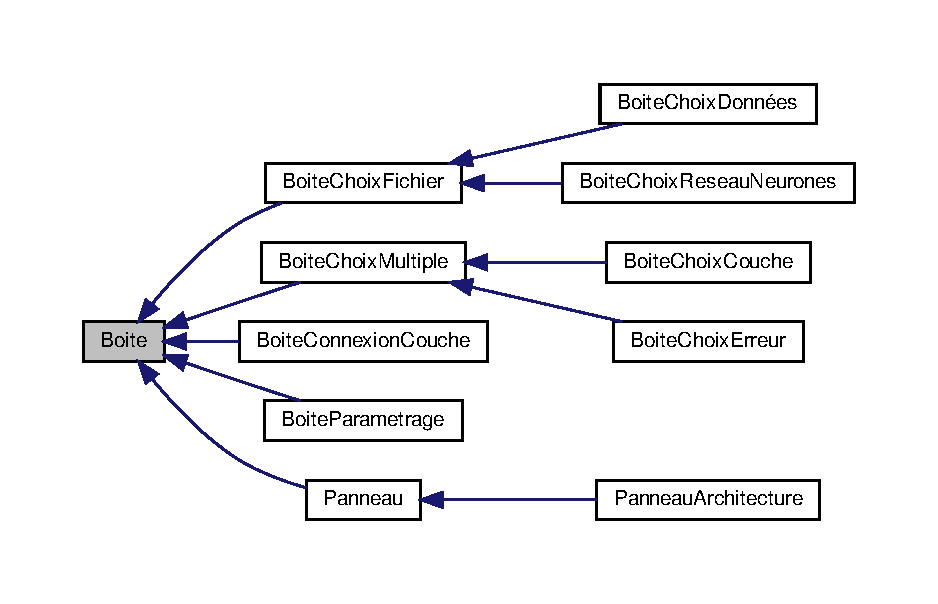
\includegraphics[width=350pt]{class_boite__inherit__graph}
\end{center}
\end{figure}
\subsection*{Fonctions membres publiques}
\begin{DoxyCompactItemize}
\item 
\mbox{\Hypertarget{class_boite_abb48ea45974db03f2c1793a7db214d82}\label{class_boite_abb48ea45974db03f2c1793a7db214d82}} 
\hyperlink{class_boite_abb48ea45974db03f2c1793a7db214d82}{Boite} (string nom)
\begin{DoxyCompactList}\small\item\em Constructeur d\textquotesingle{}une boite avec un nom. \end{DoxyCompactList}\end{DoxyCompactItemize}


\subsection{Description détaillée}
Gestion du type \hyperlink{class_boite}{Boite}. 

\begin{DoxyAuthor}{Auteur}
Samra 
\end{DoxyAuthor}
\begin{DoxyVersion}{Version}
1.\+0 
\end{DoxyVersion}
\begin{DoxyDate}{Date}
avril 2019
\end{DoxyDate}
Cette classe hérite de getkmm\+::\+Frame 

Définition à la ligne 19 du fichier Boite.\+hpp.



La documentation de cette classe a été générée à partir du fichier suivant \+:\begin{DoxyCompactItemize}
\item 
src/ihm/Boite.\+hpp\end{DoxyCompactItemize}

\hypertarget{class_boite_architecture}{}\section{Référence de la classe Boite\+Architecture}
\label{class_boite_architecture}\index{Boite\+Architecture@{Boite\+Architecture}}


Gestion de l\textquotesingle{}interaction Homme/\+Machine liée au choix de l architecture.  




{\ttfamily \#include $<$Boite\+Architecture.\+hpp$>$}



\subsection{Description détaillée}
Gestion de l\textquotesingle{}interaction Homme/\+Machine liée au choix de l architecture. 

\begin{DoxyAuthor}{Auteur}
Marion 
\end{DoxyAuthor}
\begin{DoxyVersion}{Version}
1.\+0 
\end{DoxyVersion}
\begin{DoxyDate}{Date}
avril 2019
\end{DoxyDate}
Ce module gere le choix de l architecture du reseau de neurones utilisé par le logiciel Cette classe hérite de \hyperlink{class_boite}{Boite} 

La documentation de cette classe a été générée à partir du fichier suivant \+:\begin{DoxyCompactItemize}
\item 
src/ihm/Boite\+Architecture.\+hpp\end{DoxyCompactItemize}

\hypertarget{class_boite_choix_couche}{}\section{Référence de la classe Boite\+Choix\+Couche}
\label{class_boite_choix_couche}\index{Boite\+Choix\+Couche@{Boite\+Choix\+Couche}}


Gestion de l\textquotesingle{}interaction Homme/\+Machine liée au choix des couches.  




{\ttfamily \#include $<$Boite\+Choix\+Couche.\+hpp$>$}



Graphe d\textquotesingle{}héritage de Boite\+Choix\+Couche\+:\nopagebreak
\begin{figure}[H]
\begin{center}
\leavevmode
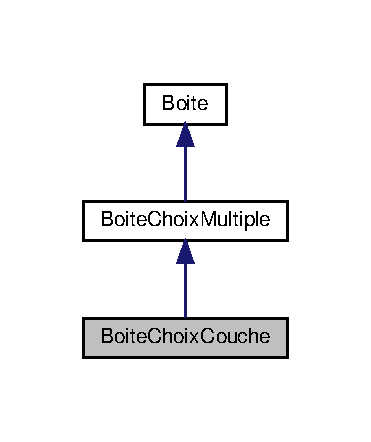
\includegraphics[width=178pt]{class_boite_choix_couche__inherit__graph}
\end{center}
\end{figure}


Graphe de collaboration de Boite\+Choix\+Couche\+:\nopagebreak
\begin{figure}[H]
\begin{center}
\leavevmode
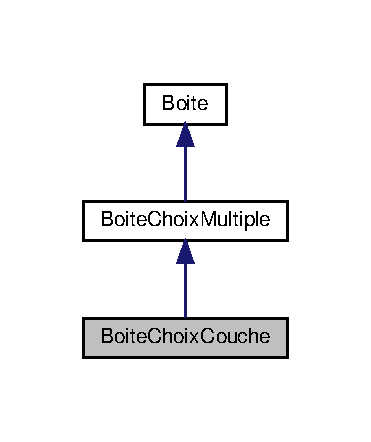
\includegraphics[width=178pt]{class_boite_choix_couche__coll__graph}
\end{center}
\end{figure}
\subsection*{Membres hérités additionnels}


\subsection{Description détaillée}
Gestion de l\textquotesingle{}interaction Homme/\+Machine liée au choix des couches. 

\begin{DoxyAuthor}{Auteur}
Samra 
\end{DoxyAuthor}
\begin{DoxyVersion}{Version}
1.\+0 
\end{DoxyVersion}
\begin{DoxyDate}{Date}
avril 2019
\end{DoxyDate}
Cette classe permet d\textquotesingle{}indiquer à l\textquotesingle{}utililsateur les differentes couches qu\textquotesingle{}il peut modifier et permet d\textquotesingle{}acceder à celle qu\textquotesingle{}il choisit Cette classe hérite de \hyperlink{class_boite_choix_multiple}{Boite\+Choix\+Multiple} 

Définition à la ligne 19 du fichier Boite\+Choix\+Couche.\+hpp.



La documentation de cette classe a été générée à partir du fichier suivant \+:\begin{DoxyCompactItemize}
\item 
src/ihm/Boite\+Choix\+Couche.\+hpp\end{DoxyCompactItemize}

\hypertarget{class_boite_choix_donnees}{}\section{Référence de la classe Boite\+Choix\+Donnees}
\label{class_boite_choix_donnees}\index{Boite\+Choix\+Donnees@{Boite\+Choix\+Donnees}}


Gestion de l\textquotesingle{}interaction Homme/\+Machine liée au choix du fichier de données.  




{\ttfamily \#include $<$Boite\+Choix\+Donnees.\+hpp$>$}



\subsection{Description détaillée}
Gestion de l\textquotesingle{}interaction Homme/\+Machine liée au choix du fichier de données. 

\begin{DoxyAuthor}{Auteur}
Samra 
\end{DoxyAuthor}
\begin{DoxyVersion}{Version}
1.\+0 
\end{DoxyVersion}
\begin{DoxyDate}{Date}
avril 2019
\end{DoxyDate}
Ce module gere le choix des fichiers de données utilisés par le logiciel Cette classe hérite de \hyperlink{class_boite_choix_fichier}{Boite\+Choix\+Fichier} 

La documentation de cette classe a été générée à partir du fichier suivant \+:\begin{DoxyCompactItemize}
\item 
src/ihm/Boite\+Choix\+Donnees.\+hpp\end{DoxyCompactItemize}

\hypertarget{class_boite_choix_donn_xC3_xA9es}{}\section{Référence de la classe Boite\+Choix\+Données}
\label{class_boite_choix_donn_xC3_xA9es}\index{Boite\+Choix\+Données@{Boite\+Choix\+Données}}


Graphe d\textquotesingle{}héritage de Boite\+Choix\+Données\+:\nopagebreak
\begin{figure}[H]
\begin{center}
\leavevmode
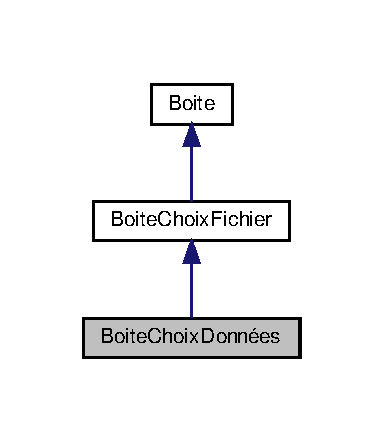
\includegraphics[width=184pt]{class_boite_choix_donn_xC3_xA9es__inherit__graph}
\end{center}
\end{figure}


Graphe de collaboration de Boite\+Choix\+Données\+:\nopagebreak
\begin{figure}[H]
\begin{center}
\leavevmode
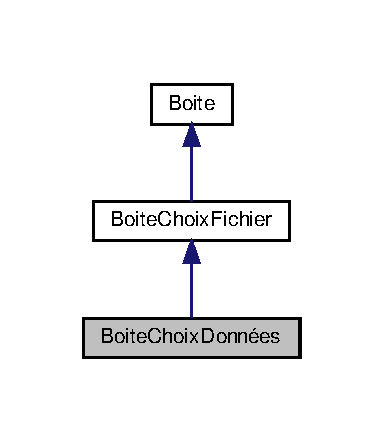
\includegraphics[width=184pt]{class_boite_choix_donn_xC3_xA9es__coll__graph}
\end{center}
\end{figure}
\subsection*{Membres hérités additionnels}


\subsection{Description détaillée}


Définition à la ligne 20 du fichier Boite\+Choix\+Donnees.\+hpp.



La documentation de cette classe a été générée à partir du fichier suivant \+:\begin{DoxyCompactItemize}
\item 
src/ihm/Boite\+Choix\+Donnees.\+hpp\end{DoxyCompactItemize}

\hypertarget{class_boite_choix_erreur}{}\section{Référence de la classe Boite\+Choix\+Erreur}
\label{class_boite_choix_erreur}\index{Boite\+Choix\+Erreur@{Boite\+Choix\+Erreur}}


Gestion de l\textquotesingle{}interaction Homme/\+Machine liée au choix de l\textquotesingle{}erreur.  




{\ttfamily \#include $<$Boite\+Choix\+Erreur.\+hpp$>$}



Graphe d\textquotesingle{}héritage de Boite\+Choix\+Erreur\+:\nopagebreak
\begin{figure}[H]
\begin{center}
\leavevmode
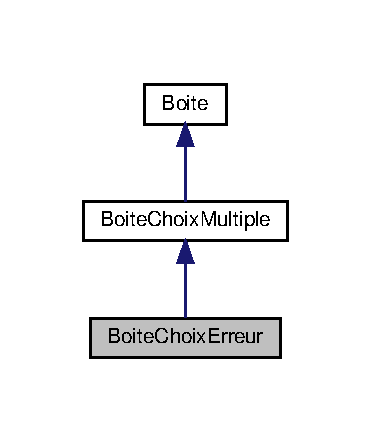
\includegraphics[width=178pt]{class_boite_choix_erreur__inherit__graph}
\end{center}
\end{figure}


Graphe de collaboration de Boite\+Choix\+Erreur\+:\nopagebreak
\begin{figure}[H]
\begin{center}
\leavevmode
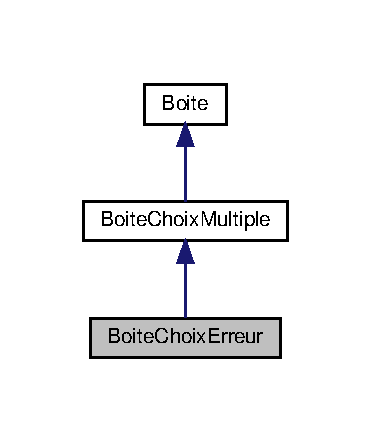
\includegraphics[width=178pt]{class_boite_choix_erreur__coll__graph}
\end{center}
\end{figure}
\subsection*{Membres hérités additionnels}


\subsection{Description détaillée}
Gestion de l\textquotesingle{}interaction Homme/\+Machine liée au choix de l\textquotesingle{}erreur. 

\begin{DoxyAuthor}{Auteur}
Samra 
\end{DoxyAuthor}
\begin{DoxyVersion}{Version}
1.\+0 
\end{DoxyVersion}
\begin{DoxyDate}{Date}
avril 2019
\end{DoxyDate}
Cette classe permet à l\textquotesingle{}utilisateur de choisir la maniere dont il veut quantifier l\textquotesingle{}erreur Cette classe hérite de \hyperlink{class_boite_choix_multiple}{Boite\+Choix\+Multiple} 

Définition à la ligne 19 du fichier Boite\+Choix\+Erreur.\+hpp.



La documentation de cette classe a été générée à partir du fichier suivant \+:\begin{DoxyCompactItemize}
\item 
src/ihm/Boite\+Choix\+Erreur.\+hpp\end{DoxyCompactItemize}

\hypertarget{class_boite_choix_fichier}{}\section{Référence de la classe Boite\+Choix\+Fichier}
\label{class_boite_choix_fichier}\index{Boite\+Choix\+Fichier@{Boite\+Choix\+Fichier}}


Gestion de l\textquotesingle{}interaction Homme/\+Machine liée au choix de fichier.  




{\ttfamily \#include $<$Boite\+Choix\+Fichier.\+hpp$>$}



Graphe d\textquotesingle{}héritage de Boite\+Choix\+Fichier\+:\nopagebreak
\begin{figure}[H]
\begin{center}
\leavevmode
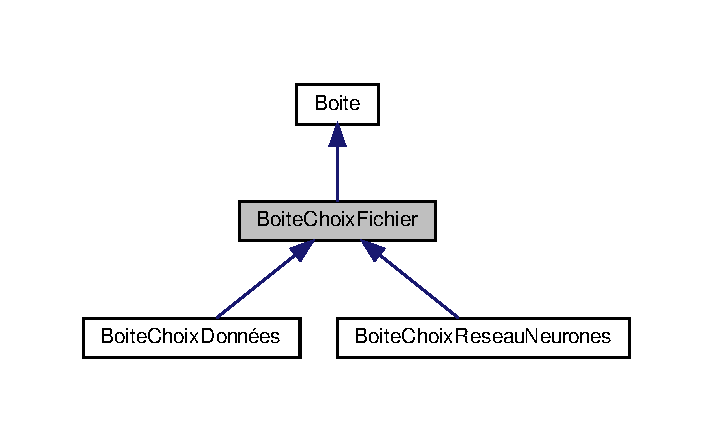
\includegraphics[width=342pt]{class_boite_choix_fichier__inherit__graph}
\end{center}
\end{figure}


Graphe de collaboration de Boite\+Choix\+Fichier\+:\nopagebreak
\begin{figure}[H]
\begin{center}
\leavevmode
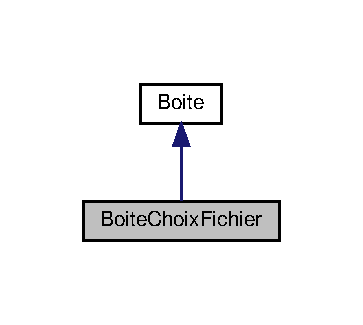
\includegraphics[width=174pt]{class_boite_choix_fichier__coll__graph}
\end{center}
\end{figure}
\subsection*{Fonctions membres publiques}
\begin{DoxyCompactItemize}
\item 
\hyperlink{class_boite_choix_fichier_a083c181fc64db190094be5bc3803e52b}{Boite\+Choix\+Fichier} (\hyperlink{class_panneau}{Panneau} parent)
\begin{DoxyCompactList}\small\item\em Constucteur prenant en paramètre un \hyperlink{class_panneau}{Panneau}. \end{DoxyCompactList}\item 
string \hyperlink{class_boite_choix_fichier_a0e051fe462c74d12ecea8a1c3bd7fad5}{get\+Nom\+Fichier} ()
\begin{DoxyCompactList}\small\item\em getteur permettant d\textquotesingle{}acceder au nom du fichier en attribut \end{DoxyCompactList}\end{DoxyCompactItemize}


\subsection{Description détaillée}
Gestion de l\textquotesingle{}interaction Homme/\+Machine liée au choix de fichier. 

Gestion de l\textquotesingle{}interaction Homme/\+Machine liée au choix des paramètres.

\begin{DoxyAuthor}{Auteur}
Samra 
\end{DoxyAuthor}
\begin{DoxyVersion}{Version}
1.\+0 
\end{DoxyVersion}
\begin{DoxyDate}{Date}
avril 2019
\end{DoxyDate}
Ce module gere le choix des fichiers (de donnée ou de reseau de neurones) utilisés par le logiciel Cette classe hérite de \hyperlink{class_boite}{Boite}

\begin{DoxyAuthor}{Auteur}
Samra 
\end{DoxyAuthor}
\begin{DoxyVersion}{Version}
1.\+0 
\end{DoxyVersion}
\begin{DoxyDate}{Date}
avril 2019
\end{DoxyDate}
Cette classe hérite de \hyperlink{class_boite}{Boite} 

Définition à la ligne 21 du fichier Boite\+Choix\+Fichier.\+hpp.



\subsection{Documentation des constructeurs et destructeur}
\mbox{\Hypertarget{class_boite_choix_fichier_a083c181fc64db190094be5bc3803e52b}\label{class_boite_choix_fichier_a083c181fc64db190094be5bc3803e52b}} 
\index{Boite\+Choix\+Fichier@{Boite\+Choix\+Fichier}!Boite\+Choix\+Fichier@{Boite\+Choix\+Fichier}}
\index{Boite\+Choix\+Fichier@{Boite\+Choix\+Fichier}!Boite\+Choix\+Fichier@{Boite\+Choix\+Fichier}}
\subsubsection{\texorpdfstring{Boite\+Choix\+Fichier()}{BoiteChoixFichier()}}
{\footnotesize\ttfamily Boite\+Choix\+Fichier\+::\+Boite\+Choix\+Fichier (\begin{DoxyParamCaption}\item[{\hyperlink{class_panneau}{Panneau}}]{parent }\end{DoxyParamCaption})}



Constucteur prenant en paramètre un \hyperlink{class_panneau}{Panneau}. 


\begin{DoxyParams}{Paramètres}
{\em parent} & un \hyperlink{class_panneau}{Panneau} préalablement défini \\
\hline
\end{DoxyParams}


\subsection{Documentation des fonctions membres}
\mbox{\Hypertarget{class_boite_choix_fichier_a0e051fe462c74d12ecea8a1c3bd7fad5}\label{class_boite_choix_fichier_a0e051fe462c74d12ecea8a1c3bd7fad5}} 
\index{Boite\+Choix\+Fichier@{Boite\+Choix\+Fichier}!get\+Nom\+Fichier@{get\+Nom\+Fichier}}
\index{get\+Nom\+Fichier@{get\+Nom\+Fichier}!Boite\+Choix\+Fichier@{Boite\+Choix\+Fichier}}
\subsubsection{\texorpdfstring{get\+Nom\+Fichier()}{getNomFichier()}}
{\footnotesize\ttfamily Boite\+Choix\+Fichier\+::get\+Nom\+Fichier (\begin{DoxyParamCaption}{ }\end{DoxyParamCaption})}



getteur permettant d\textquotesingle{}acceder au nom du fichier en attribut 

\begin{DoxyReturn}{Renvoie}
le string correspondant au nom du fichier 
\end{DoxyReturn}


La documentation de cette classe a été générée à partir du fichier suivant \+:\begin{DoxyCompactItemize}
\item 
src/ihm/Boite\+Choix\+Fichier.\+hpp\end{DoxyCompactItemize}

\hypertarget{class_boite_choix_multiple}{}\section{Référence de la classe Boite\+Choix\+Multiple}
\label{class_boite_choix_multiple}\index{Boite\+Choix\+Multiple@{Boite\+Choix\+Multiple}}


Gestion de l\textquotesingle{}interaction Homme/\+Machine liée au choix de l\textquotesingle{}utilisateur.  




{\ttfamily \#include $<$Boite\+Choix\+Multiple.\+hpp$>$}



Graphe d\textquotesingle{}héritage de Boite\+Choix\+Multiple\+:\nopagebreak
\begin{figure}[H]
\begin{center}
\leavevmode
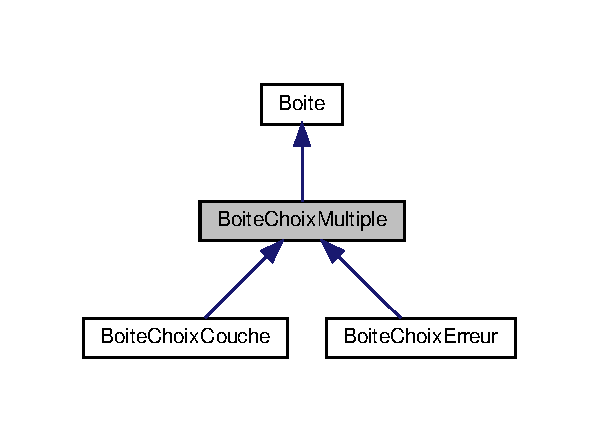
\includegraphics[width=288pt]{class_boite_choix_multiple__inherit__graph}
\end{center}
\end{figure}


Graphe de collaboration de Boite\+Choix\+Multiple\+:\nopagebreak
\begin{figure}[H]
\begin{center}
\leavevmode
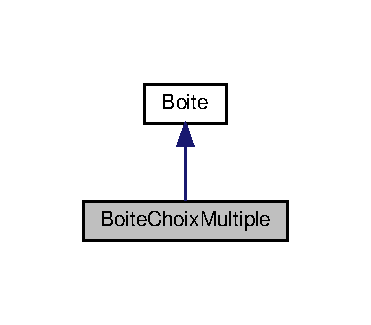
\includegraphics[width=178pt]{class_boite_choix_multiple__coll__graph}
\end{center}
\end{figure}
\subsection*{Fonctions membres publiques}
\begin{DoxyCompactItemize}
\item 
\hyperlink{class_boite_choix_multiple_a33c5d1f1b62448952ea8503cdb7ade50}{Boite\+Choix\+Multiple} (string nom)
\begin{DoxyCompactList}\small\item\em Constucteur prenant en paramètre un string. \end{DoxyCompactList}\item 
void \hyperlink{class_boite_choix_multiple_aa0acac137fd87665bc4225e1eec6e387}{ajouter\+Choix} (string nom)
\begin{DoxyCompactList}\small\item\em Méthode permettant d\textquotesingle{}ajouter un string correpondant à un nouveau choix au vecteur de choix. \end{DoxyCompactList}\item 
void \hyperlink{class_boite_choix_multiple_a52c59e771b17233ba4e1816907a68284}{ajouter\+Choix} (vector$<$ string $>$ liste\+\_\+nom)
\begin{DoxyCompactList}\small\item\em Méthode permettant d\textquotesingle{}ajouter un plusieur string correpondant à des nouveaux choix au vecteur de choix. \end{DoxyCompactList}\item 
void \hyperlink{class_boite_choix_multiple_ab37e456d084fb9e70d7e24df0839916f}{supprimer\+Choix} (string nom)
\begin{DoxyCompactList}\small\item\em Méthode permettant de supprimer un choix du vecteur de choix. \end{DoxyCompactList}\item 
string \hyperlink{class_boite_choix_multiple_a3766802fe49f850dbda7a6bdbcb2d5d7}{get\+Valeur\+Sectionnee} ()
\begin{DoxyCompactList}\small\item\em Méthode permettant la lecture du choix de l\textquotesingle{}utilisateur. \end{DoxyCompactList}\end{DoxyCompactItemize}


\subsection{Description détaillée}
Gestion de l\textquotesingle{}interaction Homme/\+Machine liée au choix de l\textquotesingle{}utilisateur. 

\begin{DoxyAuthor}{Auteur}
Samra 
\end{DoxyAuthor}
\begin{DoxyVersion}{Version}
1.\+0 
\end{DoxyVersion}
\begin{DoxyDate}{Date}
avril 2019
\end{DoxyDate}
Cette classe permet d\textquotesingle{}indiquer à l\textquotesingle{}utililsateur les differentes options qui lui sont proposées et permet d\textquotesingle{}acceder à celle qu\textquotesingle{}il choisit Cette classe hérite de \hyperlink{class_boite}{Boite} 

Définition à la ligne 20 du fichier Boite\+Choix\+Multiple.\+hpp.



\subsection{Documentation des constructeurs et destructeur}
\mbox{\Hypertarget{class_boite_choix_multiple_a33c5d1f1b62448952ea8503cdb7ade50}\label{class_boite_choix_multiple_a33c5d1f1b62448952ea8503cdb7ade50}} 
\index{Boite\+Choix\+Multiple@{Boite\+Choix\+Multiple}!Boite\+Choix\+Multiple@{Boite\+Choix\+Multiple}}
\index{Boite\+Choix\+Multiple@{Boite\+Choix\+Multiple}!Boite\+Choix\+Multiple@{Boite\+Choix\+Multiple}}
\subsubsection{\texorpdfstring{Boite\+Choix\+Multiple()}{BoiteChoixMultiple()}}
{\footnotesize\ttfamily Boite\+Choix\+Multiple\+::\+Boite\+Choix\+Multiple (\begin{DoxyParamCaption}\item[{string}]{nom }\end{DoxyParamCaption})}



Constucteur prenant en paramètre un string. 


\begin{DoxyParams}{Paramètres}
{\em Un} & string correspondant à un premier choix offert à l\textquotesingle{}utilisateur \\
\hline
\end{DoxyParams}


\subsection{Documentation des fonctions membres}
\mbox{\Hypertarget{class_boite_choix_multiple_aa0acac137fd87665bc4225e1eec6e387}\label{class_boite_choix_multiple_aa0acac137fd87665bc4225e1eec6e387}} 
\index{Boite\+Choix\+Multiple@{Boite\+Choix\+Multiple}!ajouter\+Choix@{ajouter\+Choix}}
\index{ajouter\+Choix@{ajouter\+Choix}!Boite\+Choix\+Multiple@{Boite\+Choix\+Multiple}}
\subsubsection{\texorpdfstring{ajouter\+Choix()}{ajouterChoix()}\hspace{0.1cm}{\footnotesize\ttfamily [1/2]}}
{\footnotesize\ttfamily Boite\+Choix\+Multiple\+::ajouter\+Choix (\begin{DoxyParamCaption}\item[{string}]{nom }\end{DoxyParamCaption})}



Méthode permettant d\textquotesingle{}ajouter un string correpondant à un nouveau choix au vecteur de choix. 


\begin{DoxyParams}{Paramètres}
{\em Un} & string correspondant au nom du nouveau choix \\
\hline
\end{DoxyParams}
\mbox{\Hypertarget{class_boite_choix_multiple_a52c59e771b17233ba4e1816907a68284}\label{class_boite_choix_multiple_a52c59e771b17233ba4e1816907a68284}} 
\index{Boite\+Choix\+Multiple@{Boite\+Choix\+Multiple}!ajouter\+Choix@{ajouter\+Choix}}
\index{ajouter\+Choix@{ajouter\+Choix}!Boite\+Choix\+Multiple@{Boite\+Choix\+Multiple}}
\subsubsection{\texorpdfstring{ajouter\+Choix()}{ajouterChoix()}\hspace{0.1cm}{\footnotesize\ttfamily [2/2]}}
{\footnotesize\ttfamily Boite\+Choix\+Multiple\+::ajouter\+Choix (\begin{DoxyParamCaption}\item[{vector$<$ string $>$}]{liste\+\_\+nom }\end{DoxyParamCaption})}



Méthode permettant d\textquotesingle{}ajouter un plusieur string correpondant à des nouveaux choix au vecteur de choix. 


\begin{DoxyParams}{Paramètres}
{\em liste\+\_\+nom} & le vecteur contenant les nouveaux noms de choix \\
\hline
\end{DoxyParams}
\mbox{\Hypertarget{class_boite_choix_multiple_a3766802fe49f850dbda7a6bdbcb2d5d7}\label{class_boite_choix_multiple_a3766802fe49f850dbda7a6bdbcb2d5d7}} 
\index{Boite\+Choix\+Multiple@{Boite\+Choix\+Multiple}!get\+Valeur\+Sectionnee@{get\+Valeur\+Sectionnee}}
\index{get\+Valeur\+Sectionnee@{get\+Valeur\+Sectionnee}!Boite\+Choix\+Multiple@{Boite\+Choix\+Multiple}}
\subsubsection{\texorpdfstring{get\+Valeur\+Sectionnee()}{getValeurSectionnee()}}
{\footnotesize\ttfamily Boite\+Choix\+Multiple\+::get\+Valeur\+Sectionnee (\begin{DoxyParamCaption}{ }\end{DoxyParamCaption})}



Méthode permettant la lecture du choix de l\textquotesingle{}utilisateur. 

\begin{DoxyReturn}{Renvoie}
le string choisie par l\textquotesingle{}utilisateur 
\end{DoxyReturn}
\mbox{\Hypertarget{class_boite_choix_multiple_ab37e456d084fb9e70d7e24df0839916f}\label{class_boite_choix_multiple_ab37e456d084fb9e70d7e24df0839916f}} 
\index{Boite\+Choix\+Multiple@{Boite\+Choix\+Multiple}!supprimer\+Choix@{supprimer\+Choix}}
\index{supprimer\+Choix@{supprimer\+Choix}!Boite\+Choix\+Multiple@{Boite\+Choix\+Multiple}}
\subsubsection{\texorpdfstring{supprimer\+Choix()}{supprimerChoix()}}
{\footnotesize\ttfamily Boite\+Choix\+Multiple\+::supprimer\+Choix (\begin{DoxyParamCaption}\item[{string}]{nom }\end{DoxyParamCaption})}



Méthode permettant de supprimer un choix du vecteur de choix. 


\begin{DoxyParams}{Paramètres}
{\em un} & string correspondant au nom du choix à retirer \\
\hline
\end{DoxyParams}


La documentation de cette classe a été générée à partir du fichier suivant \+:\begin{DoxyCompactItemize}
\item 
src/ihm/Boite\+Choix\+Multiple.\+hpp\end{DoxyCompactItemize}

\hypertarget{class_boite_choix_reseau_neurones}{}\section{Référence de la classe Boite\+Choix\+Reseau\+Neurones}
\label{class_boite_choix_reseau_neurones}\index{Boite\+Choix\+Reseau\+Neurones@{Boite\+Choix\+Reseau\+Neurones}}


Gestion de l\textquotesingle{}interaction Homme/\+Machine liée au choix du fichier de RN.  




{\ttfamily \#include $<$Boite\+Choix\+Reseau\+Neurones.\+hpp$>$}



Graphe d\textquotesingle{}héritage de Boite\+Choix\+Reseau\+Neurones\+:\nopagebreak
\begin{figure}[H]
\begin{center}
\leavevmode
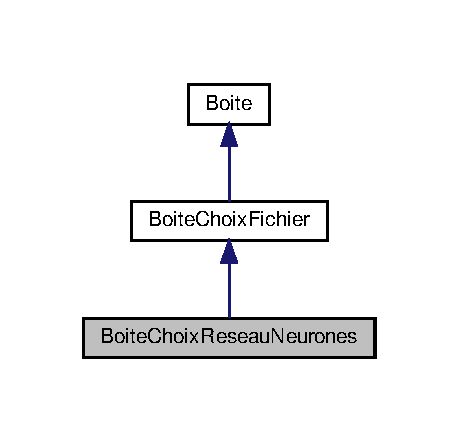
\includegraphics[width=220pt]{class_boite_choix_reseau_neurones__inherit__graph}
\end{center}
\end{figure}


Graphe de collaboration de Boite\+Choix\+Reseau\+Neurones\+:\nopagebreak
\begin{figure}[H]
\begin{center}
\leavevmode
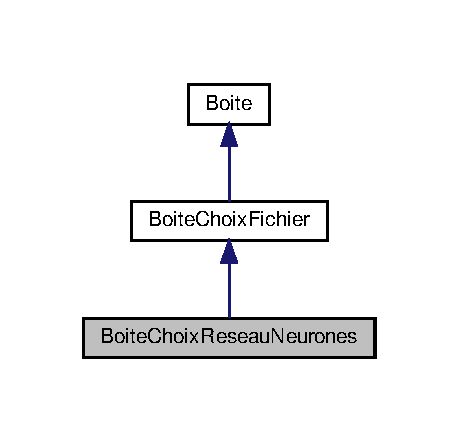
\includegraphics[width=220pt]{class_boite_choix_reseau_neurones__coll__graph}
\end{center}
\end{figure}
\subsection*{Membres hérités additionnels}


\subsection{Description détaillée}
Gestion de l\textquotesingle{}interaction Homme/\+Machine liée au choix du fichier de RN. 

\begin{DoxyAuthor}{Auteur}
Samra 
\end{DoxyAuthor}
\begin{DoxyVersion}{Version}
1.\+0 
\end{DoxyVersion}
\begin{DoxyDate}{Date}
avril 2019
\end{DoxyDate}
Ce module gere le choix des fichiers de reseau de neurones utilisés par le logiciel Cette classe hérite de \hyperlink{class_boite_choix_fichier}{Boite\+Choix\+Fichier} 

Définition à la ligne 20 du fichier Boite\+Choix\+Reseau\+Neurones.\+hpp.



La documentation de cette classe a été générée à partir du fichier suivant \+:\begin{DoxyCompactItemize}
\item 
src/ihm/Boite\+Choix\+Reseau\+Neurones.\+hpp\end{DoxyCompactItemize}

\hypertarget{class_boite_connexion_couche}{}\section{Référence de la classe Boite\+Connexion\+Couche}
\label{class_boite_connexion_couche}\index{Boite\+Connexion\+Couche@{Boite\+Connexion\+Couche}}


Gestion de l\textquotesingle{}interaction Homme/\+Machine liée à la liaison entre 2 couches.  




{\ttfamily \#include $<$Boite\+Connexion\+Couche.\+hpp$>$}



Graphe d\textquotesingle{}héritage de Boite\+Connexion\+Couche\+:\nopagebreak
\begin{figure}[H]
\begin{center}
\leavevmode
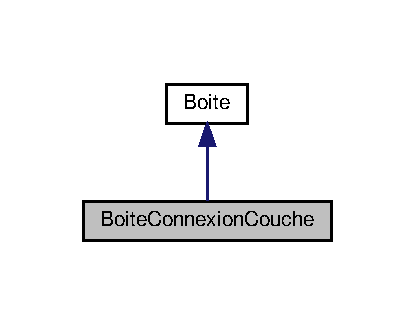
\includegraphics[width=199pt]{class_boite_connexion_couche__inherit__graph}
\end{center}
\end{figure}


Graphe de collaboration de Boite\+Connexion\+Couche\+:\nopagebreak
\begin{figure}[H]
\begin{center}
\leavevmode
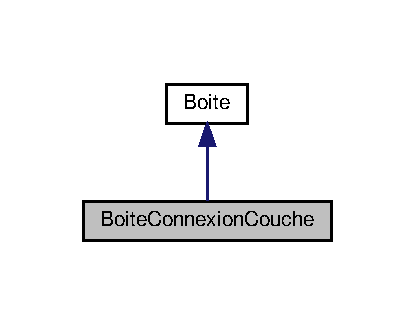
\includegraphics[width=199pt]{class_boite_connexion_couche__coll__graph}
\end{center}
\end{figure}
\subsection*{Fonctions membres publiques}
\begin{DoxyCompactItemize}
\item 
\hyperlink{class_boite_connexion_couche_a69b773ea326589e81c3beba4f8eef4e7}{Boite\+Connexion\+Couche} (\hyperlink{class_panneau}{Panneau} parent)
\begin{DoxyCompactList}\small\item\em Constucteur prenant en paramètre un \hyperlink{class_panneau}{Panneau}. \end{DoxyCompactList}\item 
void \hyperlink{class_boite_connexion_couche_aca89aac7d4ae0ba89828c6d542790925}{set\+Couche\+Initiale} (\hyperlink{class_couche}{Couche} couche)
\begin{DoxyCompactList}\small\item\em Setteur permetant de changer la valeur de la \hyperlink{class_couche}{Couche} Initiale. \end{DoxyCompactList}\item 
void \hyperlink{class_boite_connexion_couche_a9469138a3db603eddacf8757595ad6cf}{set\+Couche\+Finale} (\hyperlink{class_couche}{Couche} couche)
\begin{DoxyCompactList}\small\item\em Setteur permetant de changer la valeur de la \hyperlink{class_couche}{Couche} finale. \end{DoxyCompactList}\item 
\hyperlink{class_couche}{Couche} \hyperlink{class_boite_connexion_couche_a3b0faf67baf198a1abaafc7c469fc6d2}{get\+Couche\+Initiale} ()
\begin{DoxyCompactList}\small\item\em Getteur permetant d\textquotesingle{}obtenir la valeur de la \hyperlink{class_couche}{Couche} Initiale. \end{DoxyCompactList}\item 
\hyperlink{class_couche}{Couche} \hyperlink{class_boite_connexion_couche_af35c756dfc1f9491e2803b251f2d4434}{get\+Couche\+Finale} ()
\begin{DoxyCompactList}\small\item\em getteur permetant d\textquotesingle{}obtenir la valeur de la \hyperlink{class_couche}{Couche} Finale \end{DoxyCompactList}\end{DoxyCompactItemize}


\subsection{Description détaillée}
Gestion de l\textquotesingle{}interaction Homme/\+Machine liée à la liaison entre 2 couches. 

\begin{DoxyAuthor}{Auteur}
Samra 
\end{DoxyAuthor}
\begin{DoxyVersion}{Version}
1.\+0 
\end{DoxyVersion}
\begin{DoxyDate}{Date}
avril 2019
\end{DoxyDate}
Module permettant le choix des couches à relier et la mise en place de leur liaison 

Définition à la ligne 21 du fichier Boite\+Connexion\+Couche.\+hpp.



\subsection{Documentation des constructeurs et destructeur}
\mbox{\Hypertarget{class_boite_connexion_couche_a69b773ea326589e81c3beba4f8eef4e7}\label{class_boite_connexion_couche_a69b773ea326589e81c3beba4f8eef4e7}} 
\index{Boite\+Connexion\+Couche@{Boite\+Connexion\+Couche}!Boite\+Connexion\+Couche@{Boite\+Connexion\+Couche}}
\index{Boite\+Connexion\+Couche@{Boite\+Connexion\+Couche}!Boite\+Connexion\+Couche@{Boite\+Connexion\+Couche}}
\subsubsection{\texorpdfstring{Boite\+Connexion\+Couche()}{BoiteConnexionCouche()}}
{\footnotesize\ttfamily Boite\+Connexion\+Couche\+::\+Boite\+Connexion\+Couche (\begin{DoxyParamCaption}\item[{\hyperlink{class_panneau}{Panneau}}]{parent }\end{DoxyParamCaption})}



Constucteur prenant en paramètre un \hyperlink{class_panneau}{Panneau}. 


\begin{DoxyParams}{Paramètres}
{\em parent} & un \hyperlink{class_panneau}{Panneau} contenant déja un réseau de neurones \\
\hline
\end{DoxyParams}


\subsection{Documentation des fonctions membres}
\mbox{\Hypertarget{class_boite_connexion_couche_af35c756dfc1f9491e2803b251f2d4434}\label{class_boite_connexion_couche_af35c756dfc1f9491e2803b251f2d4434}} 
\index{Boite\+Connexion\+Couche@{Boite\+Connexion\+Couche}!get\+Couche\+Finale@{get\+Couche\+Finale}}
\index{get\+Couche\+Finale@{get\+Couche\+Finale}!Boite\+Connexion\+Couche@{Boite\+Connexion\+Couche}}
\subsubsection{\texorpdfstring{get\+Couche\+Finale()}{getCoucheFinale()}}
{\footnotesize\ttfamily Boite\+Connexion\+Couche\+::get\+Couche\+Finale (\begin{DoxyParamCaption}{ }\end{DoxyParamCaption})}



getteur permetant d\textquotesingle{}obtenir la valeur de la \hyperlink{class_couche}{Couche} Finale 

\begin{DoxyReturn}{Renvoie}
la \hyperlink{class_couche}{Couche} c\+\_\+finale en attribut de la classe 
\end{DoxyReturn}
\mbox{\Hypertarget{class_boite_connexion_couche_a3b0faf67baf198a1abaafc7c469fc6d2}\label{class_boite_connexion_couche_a3b0faf67baf198a1abaafc7c469fc6d2}} 
\index{Boite\+Connexion\+Couche@{Boite\+Connexion\+Couche}!get\+Couche\+Initiale@{get\+Couche\+Initiale}}
\index{get\+Couche\+Initiale@{get\+Couche\+Initiale}!Boite\+Connexion\+Couche@{Boite\+Connexion\+Couche}}
\subsubsection{\texorpdfstring{get\+Couche\+Initiale()}{getCoucheInitiale()}}
{\footnotesize\ttfamily Boite\+Connexion\+Couche\+::get\+Couche\+Initiale (\begin{DoxyParamCaption}{ }\end{DoxyParamCaption})}



Getteur permetant d\textquotesingle{}obtenir la valeur de la \hyperlink{class_couche}{Couche} Initiale. 

\begin{DoxyReturn}{Renvoie}
la \hyperlink{class_couche}{Couche} c\+\_\+init en attribut de la classe 
\end{DoxyReturn}
\mbox{\Hypertarget{class_boite_connexion_couche_a9469138a3db603eddacf8757595ad6cf}\label{class_boite_connexion_couche_a9469138a3db603eddacf8757595ad6cf}} 
\index{Boite\+Connexion\+Couche@{Boite\+Connexion\+Couche}!set\+Couche\+Finale@{set\+Couche\+Finale}}
\index{set\+Couche\+Finale@{set\+Couche\+Finale}!Boite\+Connexion\+Couche@{Boite\+Connexion\+Couche}}
\subsubsection{\texorpdfstring{set\+Couche\+Finale()}{setCoucheFinale()}}
{\footnotesize\ttfamily Boite\+Connexion\+Couche\+::set\+Couche\+Finale (\begin{DoxyParamCaption}\item[{\hyperlink{class_couche}{Couche}}]{couche }\end{DoxyParamCaption})}



Setteur permetant de changer la valeur de la \hyperlink{class_couche}{Couche} finale. 


\begin{DoxyParams}{Paramètres}
{\em la} & nouvelle \hyperlink{class_couche}{Couche} finale \\
\hline
\end{DoxyParams}
\mbox{\Hypertarget{class_boite_connexion_couche_aca89aac7d4ae0ba89828c6d542790925}\label{class_boite_connexion_couche_aca89aac7d4ae0ba89828c6d542790925}} 
\index{Boite\+Connexion\+Couche@{Boite\+Connexion\+Couche}!set\+Couche\+Initiale@{set\+Couche\+Initiale}}
\index{set\+Couche\+Initiale@{set\+Couche\+Initiale}!Boite\+Connexion\+Couche@{Boite\+Connexion\+Couche}}
\subsubsection{\texorpdfstring{set\+Couche\+Initiale()}{setCoucheInitiale()}}
{\footnotesize\ttfamily Boite\+Connexion\+Couche\+::set\+Couche\+Initiale (\begin{DoxyParamCaption}\item[{\hyperlink{class_couche}{Couche}}]{couche }\end{DoxyParamCaption})}



Setteur permetant de changer la valeur de la \hyperlink{class_couche}{Couche} Initiale. 


\begin{DoxyParams}{Paramètres}
{\em la} & nouvelle \hyperlink{class_couche}{Couche} initiale \\
\hline
\end{DoxyParams}


La documentation de cette classe a été générée à partir du fichier suivant \+:\begin{DoxyCompactItemize}
\item 
src/ihm/Boite\+Connexion\+Couche.\+hpp\end{DoxyCompactItemize}

\hypertarget{class_boite_parametrage}{}\section{Référence de la classe Boite\+Parametrage}
\label{class_boite_parametrage}\index{Boite\+Parametrage@{Boite\+Parametrage}}


Graphe d\textquotesingle{}héritage de Boite\+Parametrage\+:\nopagebreak
\begin{figure}[H]
\begin{center}
\leavevmode
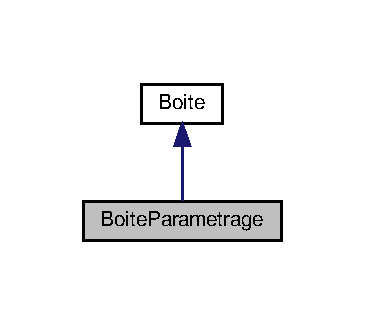
\includegraphics[width=175pt]{class_boite_parametrage__inherit__graph}
\end{center}
\end{figure}


Graphe de collaboration de Boite\+Parametrage\+:\nopagebreak
\begin{figure}[H]
\begin{center}
\leavevmode
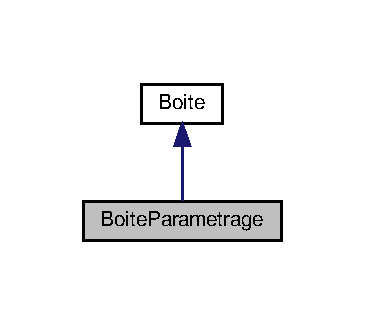
\includegraphics[width=175pt]{class_boite_parametrage__coll__graph}
\end{center}
\end{figure}
\subsection*{Fonctions membres publiques}
\begin{DoxyCompactItemize}
\item 
\hyperlink{class_boite_parametrage_a5c4d9098fac45ee4dc7ff2d6d8e910bb}{Boite\+Parametrage} (\hyperlink{class_panneau}{Panneau} parent)
\begin{DoxyCompactList}\small\item\em Constucteur prenant en paramètre un \hyperlink{class_panneau}{Panneau}. \end{DoxyCompactList}\item 
\hyperlink{class_parametres_apprentissage}{Parametres\+Apprentissage} \hyperlink{class_boite_parametrage_ad7c3de61949e05469a73e6b8369205e2}{get\+Parametrage} ()
\begin{DoxyCompactList}\small\item\em Getteur permettant d\textquotesingle{}acceder aux paramètres en attribut. \end{DoxyCompactList}\end{DoxyCompactItemize}


\subsection{Description détaillée}


Définition à la ligne 19 du fichier Boite\+Parametrage.\+hpp.



\subsection{Documentation des constructeurs et destructeur}
\mbox{\Hypertarget{class_boite_parametrage_a5c4d9098fac45ee4dc7ff2d6d8e910bb}\label{class_boite_parametrage_a5c4d9098fac45ee4dc7ff2d6d8e910bb}} 
\index{Boite\+Parametrage@{Boite\+Parametrage}!Boite\+Parametrage@{Boite\+Parametrage}}
\index{Boite\+Parametrage@{Boite\+Parametrage}!Boite\+Parametrage@{Boite\+Parametrage}}
\subsubsection{\texorpdfstring{Boite\+Parametrage()}{BoiteParametrage()}}
{\footnotesize\ttfamily Boite\+Parametrage\+::\+Boite\+Parametrage (\begin{DoxyParamCaption}\item[{\hyperlink{class_panneau}{Panneau}}]{parent }\end{DoxyParamCaption})}



Constucteur prenant en paramètre un \hyperlink{class_panneau}{Panneau}. 


\begin{DoxyParams}{Paramètres}
{\em parent} & un \hyperlink{class_panneau}{Panneau} contenant déja un réseau de neurones \\
\hline
\end{DoxyParams}


\subsection{Documentation des fonctions membres}
\mbox{\Hypertarget{class_boite_parametrage_ad7c3de61949e05469a73e6b8369205e2}\label{class_boite_parametrage_ad7c3de61949e05469a73e6b8369205e2}} 
\index{Boite\+Parametrage@{Boite\+Parametrage}!get\+Parametrage@{get\+Parametrage}}
\index{get\+Parametrage@{get\+Parametrage}!Boite\+Parametrage@{Boite\+Parametrage}}
\subsubsection{\texorpdfstring{get\+Parametrage()}{getParametrage()}}
{\footnotesize\ttfamily Boite\+Parametrage\+::get\+Parametrage (\begin{DoxyParamCaption}{ }\end{DoxyParamCaption})}



Getteur permettant d\textquotesingle{}acceder aux paramètres en attribut. 

\begin{DoxyReturn}{Renvoie}
\hyperlink{class_parametres_apprentissage}{Parametres\+Apprentissage} 
\end{DoxyReturn}


La documentation de cette classe a été générée à partir du fichier suivant \+:\begin{DoxyCompactItemize}
\item 
src/ihm/Boite\+Parametrage.\+hpp\end{DoxyCompactItemize}

\hypertarget{class_couche}{}\section{Référence de la classe Couche}
\label{class_couche}\index{Couche@{Couche}}


Classe liée à la couche.  




{\ttfamily \#include $<$Couche.\+hpp$>$}



Graphe d\textquotesingle{}héritage de Couche\+:\nopagebreak
\begin{figure}[H]
\begin{center}
\leavevmode
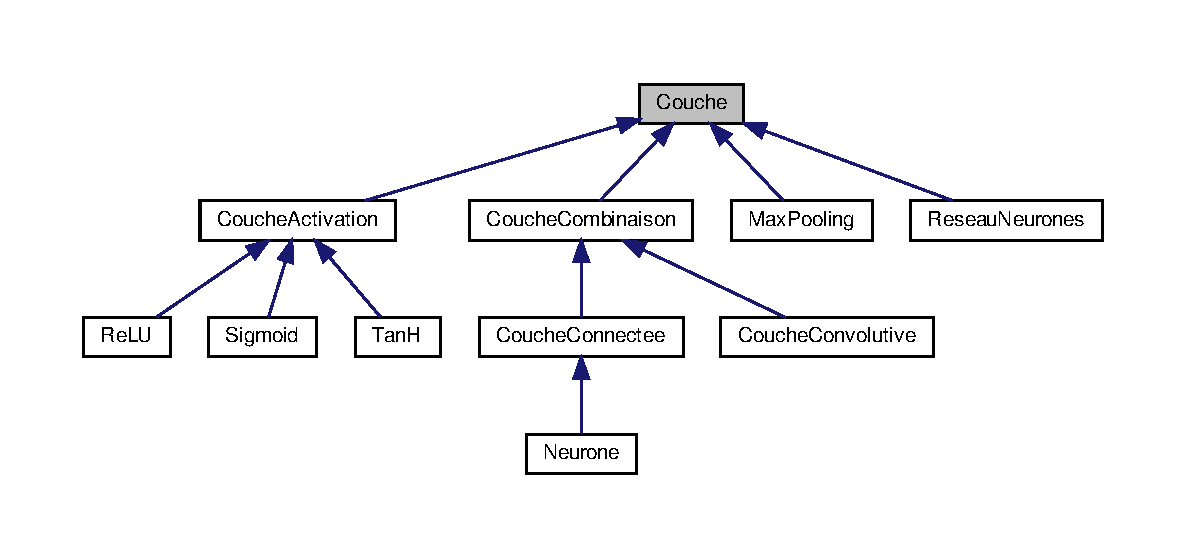
\includegraphics[width=350pt]{class_couche__inherit__graph}
\end{center}
\end{figure}
\subsection*{Fonctions membres publiques}
\begin{DoxyCompactItemize}
\item 
\mbox{\Hypertarget{class_couche_a6da95828f8c597f57aaac057b9357622}\label{class_couche_a6da95828f8c597f57aaac057b9357622}} 
\hyperlink{class_couche_a6da95828f8c597f57aaac057b9357622}{Couche} (\hyperlink{class_dim_tenseur}{Dim\+Tenseur} din, \hyperlink{class_dim_tenseur}{Dim\+Tenseur} dout, std\+::string no)
\begin{DoxyCompactList}\small\item\em Constructeur d\textquotesingle{}une couche à partir de la taille des tenseurs d\textquotesingle{}entrée/sortie. \end{DoxyCompactList}\item 
virtual \hyperlink{class_tenseur}{Tenseur} \hyperlink{class_couche_a1f0ed59e21020f5d4f37933af4d1b1e5}{propagation} (\hyperlink{class_tenseur}{Tenseur} t)
\begin{DoxyCompactList}\small\item\em Methode virtuelle permettant la propagation d\textquotesingle{}une couche à une autre. \end{DoxyCompactList}\item 
virtual \hyperlink{class_tenseur}{Tenseur} \hyperlink{class_couche_acfb65d035c2070d65b699508b7333bb3}{derivee} (\hyperlink{class_tenseur}{Tenseur} t)
\begin{DoxyCompactList}\small\item\em Methode virtuelle pour avoir la derivee de la couche. \end{DoxyCompactList}\item 
void \hyperlink{class_couche_ab24ce01bc6fb7b903013f7682ce60a7e}{set\+Dim\+Input} (\hyperlink{class_dim_tenseur}{Dim\+Tenseur} dim\+In)
\begin{DoxyCompactList}\small\item\em Méthode pour fixer la taille du tenseur à l\textquotesingle{}entrée de la couche. \end{DoxyCompactList}\item 
void \hyperlink{class_couche_a9af2f37eaf1063cb05abe980cfaa4cce}{set\+Dim\+Output} (\hyperlink{class_dim_tenseur}{Dim\+Tenseur} dim\+Out)
\begin{DoxyCompactList}\small\item\em Méthode pour fixer la taille du tenseur à la sortie de la couche. \end{DoxyCompactList}\item 
\hyperlink{class_dim_tenseur}{Dim\+Tenseur} \hyperlink{class_couche_a4f3e4fe4a84f2dfcbee4bda6e20bdc03}{get\+Dim\+Input} () const
\begin{DoxyCompactList}\small\item\em Méthode pour obtenir la taille du tenseur à l\textquotesingle{}entrée de la couche. \end{DoxyCompactList}\item 
\hyperlink{class_dim_tenseur}{Dim\+Tenseur} \hyperlink{class_couche_ae8c80adf3a53da0d975e6f1148d0cea9}{get\+Dim\+Output} () const
\begin{DoxyCompactList}\small\item\em Méthode pour obtenir la taille du tenseur à la sortie de la couche. \end{DoxyCompactList}\item 
std\+::string \hyperlink{class_couche_a367bb58eaafab2b5fe635e6d3350fe4b}{get\+Nom} () const
\begin{DoxyCompactList}\small\item\em Méthode pour obtenir le nom de la couche. \end{DoxyCompactList}\item 
virtual bool \hyperlink{class_couche_a3c76d2c7a0adf864dc6f3f5fbf2c7563}{afficher} ()
\begin{DoxyCompactList}\small\item\em Méthode pour savoir si la couche est affichée ou non. \end{DoxyCompactList}\end{DoxyCompactItemize}


\subsection{Description détaillée}
Classe liée à la couche. 

\begin{DoxyAuthor}{Auteur}
Adrien 
\end{DoxyAuthor}
\begin{DoxyVersion}{Version}
1.\+0 
\end{DoxyVersion}
\begin{DoxyDate}{Date}
avril 2019
\end{DoxyDate}
Cette classe permet de fixer les tailles (entrée/sortie) de la couche. Une couche peut être dérivée et propagée. 

Définition à la ligne 20 du fichier Couche.\+hpp.



\subsection{Documentation des fonctions membres}
\mbox{\Hypertarget{class_couche_a3c76d2c7a0adf864dc6f3f5fbf2c7563}\label{class_couche_a3c76d2c7a0adf864dc6f3f5fbf2c7563}} 
\index{Couche@{Couche}!afficher@{afficher}}
\index{afficher@{afficher}!Couche@{Couche}}
\subsubsection{\texorpdfstring{afficher()}{afficher()}}
{\footnotesize\ttfamily bool Couche\+::afficher (\begin{DoxyParamCaption}{ }\end{DoxyParamCaption})\hspace{0.3cm}{\ttfamily [virtual]}}



Méthode pour savoir si la couche est affichée ou non. 

\begin{DoxyReturn}{Renvoie}
booléen 
\end{DoxyReturn}


Définition à la ligne 60 du fichier Couche.\+cpp.

\mbox{\Hypertarget{class_couche_acfb65d035c2070d65b699508b7333bb3}\label{class_couche_acfb65d035c2070d65b699508b7333bb3}} 
\index{Couche@{Couche}!derivee@{derivee}}
\index{derivee@{derivee}!Couche@{Couche}}
\subsubsection{\texorpdfstring{derivee()}{derivee()}}
{\footnotesize\ttfamily void Couche\+::derivee (\begin{DoxyParamCaption}\item[{\hyperlink{class_tenseur}{Tenseur}}]{t }\end{DoxyParamCaption})\hspace{0.3cm}{\ttfamily [virtual]}}



Methode virtuelle pour avoir la derivee de la couche. 


\begin{DoxyParams}{Paramètres}
{\em t} & le tenseur pour lequel on veut la derivee \\
\hline
\end{DoxyParams}
\begin{DoxyReturn}{Renvoie}
la derivee de la couche 
\end{DoxyReturn}


Définition à la ligne 19 du fichier Couche.\+cpp.

\mbox{\Hypertarget{class_couche_a4f3e4fe4a84f2dfcbee4bda6e20bdc03}\label{class_couche_a4f3e4fe4a84f2dfcbee4bda6e20bdc03}} 
\index{Couche@{Couche}!get\+Dim\+Input@{get\+Dim\+Input}}
\index{get\+Dim\+Input@{get\+Dim\+Input}!Couche@{Couche}}
\subsubsection{\texorpdfstring{get\+Dim\+Input()}{getDimInput()}}
{\footnotesize\ttfamily \hyperlink{class_dim_tenseur}{Dim\+Tenseur} Couche\+::get\+Dim\+Input (\begin{DoxyParamCaption}{ }\end{DoxyParamCaption}) const}



Méthode pour obtenir la taille du tenseur à l\textquotesingle{}entrée de la couche. 

\begin{DoxyReturn}{Renvoie}
La taille du tenseur d\textquotesingle{}entrée 
\end{DoxyReturn}


Définition à la ligne 39 du fichier Couche.\+cpp.

\mbox{\Hypertarget{class_couche_ae8c80adf3a53da0d975e6f1148d0cea9}\label{class_couche_ae8c80adf3a53da0d975e6f1148d0cea9}} 
\index{Couche@{Couche}!get\+Dim\+Output@{get\+Dim\+Output}}
\index{get\+Dim\+Output@{get\+Dim\+Output}!Couche@{Couche}}
\subsubsection{\texorpdfstring{get\+Dim\+Output()}{getDimOutput()}}
{\footnotesize\ttfamily \hyperlink{class_dim_tenseur}{Dim\+Tenseur} Couche\+::get\+Dim\+Output (\begin{DoxyParamCaption}{ }\end{DoxyParamCaption}) const}



Méthode pour obtenir la taille du tenseur à la sortie de la couche. 

\begin{DoxyReturn}{Renvoie}
La taille du tenseur de sortie 
\end{DoxyReturn}


Définition à la ligne 46 du fichier Couche.\+cpp.

\mbox{\Hypertarget{class_couche_a367bb58eaafab2b5fe635e6d3350fe4b}\label{class_couche_a367bb58eaafab2b5fe635e6d3350fe4b}} 
\index{Couche@{Couche}!get\+Nom@{get\+Nom}}
\index{get\+Nom@{get\+Nom}!Couche@{Couche}}
\subsubsection{\texorpdfstring{get\+Nom()}{getNom()}}
{\footnotesize\ttfamily string Couche\+::get\+Nom (\begin{DoxyParamCaption}{ }\end{DoxyParamCaption}) const}



Méthode pour obtenir le nom de la couche. 

\begin{DoxyReturn}{Renvoie}
Le nom de la couche 
\end{DoxyReturn}


Définition à la ligne 53 du fichier Couche.\+cpp.

\mbox{\Hypertarget{class_couche_a1f0ed59e21020f5d4f37933af4d1b1e5}\label{class_couche_a1f0ed59e21020f5d4f37933af4d1b1e5}} 
\index{Couche@{Couche}!propagation@{propagation}}
\index{propagation@{propagation}!Couche@{Couche}}
\subsubsection{\texorpdfstring{propagation()}{propagation()}}
{\footnotesize\ttfamily \hyperlink{class_tenseur}{Tenseur} Couche\+::propagation (\begin{DoxyParamCaption}\item[{\hyperlink{class_tenseur}{Tenseur}}]{t }\end{DoxyParamCaption})\hspace{0.3cm}{\ttfamily [virtual]}}



Methode virtuelle permettant la propagation d\textquotesingle{}une couche à une autre. 


\begin{DoxyParams}{Paramètres}
{\em t} & le tenseur d\textquotesingle{}entree \\
\hline
\end{DoxyParams}
\begin{DoxyReturn}{Renvoie}
la sortie de la couche 
\end{DoxyReturn}


Réimplémentée dans \hyperlink{class_reseau_neurones_a7079f7694f0369187b8ff28cefcbc5eb}{Reseau\+Neurones}, \hyperlink{class_couche_convolutive_ad1a55b3dc9bf52e0725ae2a7b2e92aa1}{Couche\+Convolutive}, \hyperlink{class_max_pooling_a48e0258bf1f949853cfceb2726035fb8}{Max\+Pooling}, \hyperlink{class_couche_connectee_acd60c499c6c74f914795f45f3f8084d0}{Couche\+Connectee}, \hyperlink{class_re_l_u_a0d42917d6a9124571b0b467c81bce38a}{Re\+LU}, \hyperlink{class_sigmoid_a6bd1f6bbc49bd7e634dc33701aee420c}{Sigmoid}, et \hyperlink{class_tan_h_a869967c9b278c6592e6fcc04b61a5f0c}{TanH}.



Définition à la ligne 13 du fichier Couche.\+cpp.

\mbox{\Hypertarget{class_couche_ab24ce01bc6fb7b903013f7682ce60a7e}\label{class_couche_ab24ce01bc6fb7b903013f7682ce60a7e}} 
\index{Couche@{Couche}!set\+Dim\+Input@{set\+Dim\+Input}}
\index{set\+Dim\+Input@{set\+Dim\+Input}!Couche@{Couche}}
\subsubsection{\texorpdfstring{set\+Dim\+Input()}{setDimInput()}}
{\footnotesize\ttfamily void Couche\+::set\+Dim\+Input (\begin{DoxyParamCaption}\item[{\hyperlink{class_dim_tenseur}{Dim\+Tenseur}}]{dim\+In }\end{DoxyParamCaption})}



Méthode pour fixer la taille du tenseur à l\textquotesingle{}entrée de la couche. 


\begin{DoxyParams}{Paramètres}
{\em dim\+In} & La dimension du tenseur d\textquotesingle{}entrée \\
\hline
\end{DoxyParams}


Définition à la ligne 25 du fichier Couche.\+cpp.

\mbox{\Hypertarget{class_couche_a9af2f37eaf1063cb05abe980cfaa4cce}\label{class_couche_a9af2f37eaf1063cb05abe980cfaa4cce}} 
\index{Couche@{Couche}!set\+Dim\+Output@{set\+Dim\+Output}}
\index{set\+Dim\+Output@{set\+Dim\+Output}!Couche@{Couche}}
\subsubsection{\texorpdfstring{set\+Dim\+Output()}{setDimOutput()}}
{\footnotesize\ttfamily void Couche\+::set\+Dim\+Output (\begin{DoxyParamCaption}\item[{\hyperlink{class_dim_tenseur}{Dim\+Tenseur}}]{dim\+Out }\end{DoxyParamCaption})}



Méthode pour fixer la taille du tenseur à la sortie de la couche. 


\begin{DoxyParams}{Paramètres}
{\em dim\+In} & La dimension du tenseur de sortie \\
\hline
\end{DoxyParams}


Définition à la ligne 32 du fichier Couche.\+cpp.



La documentation de cette classe a été générée à partir des fichiers suivants \+:\begin{DoxyCompactItemize}
\item 
src/deeplearn/archi/Couche.\+hpp\item 
src/deeplearn/archi/Couche.\+cpp\end{DoxyCompactItemize}

\hypertarget{class_couche_activation}{}\section{Référence de la classe Couche\+Activation}
\label{class_couche_activation}\index{Couche\+Activation@{Couche\+Activation}}


Gestion d\textquotesingle{}une couche d\textquotesingle{}activation.  




{\ttfamily \#include $<$Couche\+Activation.\+hpp$>$}



Graphe d\textquotesingle{}héritage de Couche\+Activation\+:\nopagebreak
\begin{figure}[H]
\begin{center}
\leavevmode
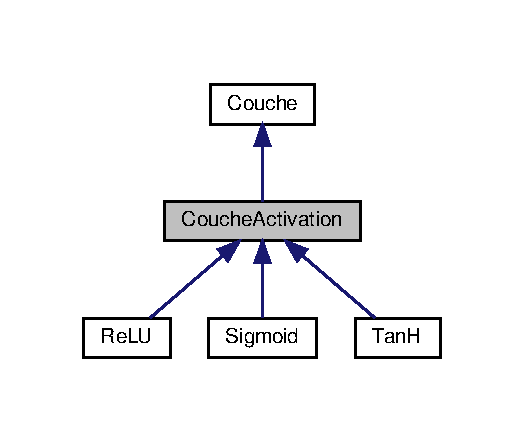
\includegraphics[width=252pt]{class_couche_activation__inherit__graph}
\end{center}
\end{figure}


Graphe de collaboration de Couche\+Activation\+:\nopagebreak
\begin{figure}[H]
\begin{center}
\leavevmode
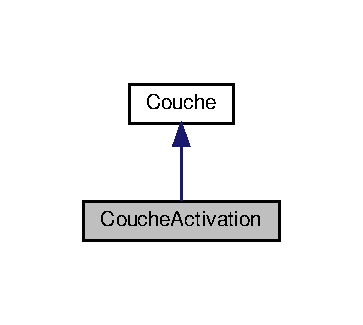
\includegraphics[width=174pt]{class_couche_activation__coll__graph}
\end{center}
\end{figure}
\subsection*{Fonctions membres publiques}
\begin{DoxyCompactItemize}
\item 
\mbox{\Hypertarget{class_couche_activation_a7ac67e43f62ade7fbf4652a64e7281e4}\label{class_couche_activation_a7ac67e43f62ade7fbf4652a64e7281e4}} 
\hyperlink{class_couche_activation_a7ac67e43f62ade7fbf4652a64e7281e4}{Couche\+Activation} (\hyperlink{class_dim_tenseur}{Dim\+Tenseur} din, \hyperlink{class_dim_tenseur}{Dim\+Tenseur} dout, std\+::string no)
\begin{DoxyCompactList}\small\item\em Constructeur d\textquotesingle{}une couche d\textquotesingle{}activation avec une dimension d\textquotesingle{}entree. \end{DoxyCompactList}\end{DoxyCompactItemize}


\subsection{Description détaillée}
Gestion d\textquotesingle{}une couche d\textquotesingle{}activation. 

\begin{DoxyAuthor}{Auteur}
Adrien 
\end{DoxyAuthor}
\begin{DoxyVersion}{Version}
1.\+0 
\end{DoxyVersion}
\begin{DoxyDate}{Date}
avril 2019
\end{DoxyDate}
Classe permettant la création d\textquotesingle{}une couche d\textquotesingle{}activation de trois types différents (sigmoid,tangente hyperbolique ou Rectified Linear Units) Cette classe hérite de la classe \hyperlink{class_couche}{Couche}. 

Définition à la ligne 18 du fichier Couche\+Activation.\+hpp.



La documentation de cette classe a été générée à partir des fichiers suivants \+:\begin{DoxyCompactItemize}
\item 
src/deeplearn/archi/Couche\+Activation.\+hpp\item 
src/deeplearn/archi/Couche\+Activation.\+cpp\end{DoxyCompactItemize}

\hypertarget{class_couche_combinaison}{}\section{Référence de la classe Couche\+Combinaison}
\label{class_couche_combinaison}\index{Couche\+Combinaison@{Couche\+Combinaison}}


Gestion d\textquotesingle{}une couche de combinaison.  




{\ttfamily \#include $<$Couche\+Combinaison.\+hpp$>$}



Graphe d\textquotesingle{}héritage de Couche\+Combinaison\+:\nopagebreak
\begin{figure}[H]
\begin{center}
\leavevmode
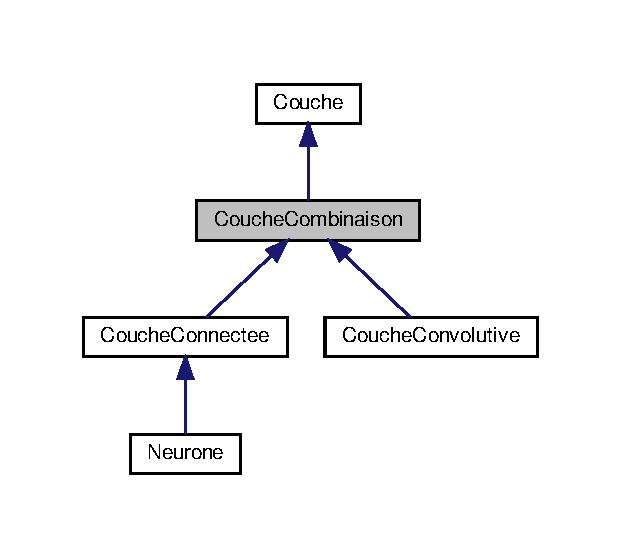
\includegraphics[width=298pt]{class_couche_combinaison__inherit__graph}
\end{center}
\end{figure}


Graphe de collaboration de Couche\+Combinaison\+:\nopagebreak
\begin{figure}[H]
\begin{center}
\leavevmode
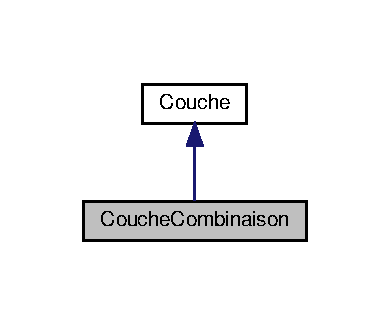
\includegraphics[width=187pt]{class_couche_combinaison__coll__graph}
\end{center}
\end{figure}
\subsection*{Fonctions membres publiques}
\begin{DoxyCompactItemize}
\item 
\mbox{\Hypertarget{class_couche_combinaison_aa28fcb2c8d4197e75b43873a0824d38f}\label{class_couche_combinaison_aa28fcb2c8d4197e75b43873a0824d38f}} 
\hyperlink{class_couche_combinaison_aa28fcb2c8d4197e75b43873a0824d38f}{Couche\+Combinaison} (\hyperlink{class_dim_tenseur}{Dim\+Tenseur} din, \hyperlink{class_dim_tenseur}{Dim\+Tenseur} dout, std\+::string no, \hyperlink{class_tenseur}{Tenseur} par)
\begin{DoxyCompactList}\small\item\em Constructeur d\textquotesingle{}une couche à partir de la taille des tenseurs d\textquotesingle{}entrée/sortie. \end{DoxyCompactList}\item 
\mbox{\Hypertarget{class_couche_combinaison_abdd34f81cb1298a4a9b2c8cef091db81}\label{class_couche_combinaison_abdd34f81cb1298a4a9b2c8cef091db81}} 
void \hyperlink{class_couche_combinaison_abdd34f81cb1298a4a9b2c8cef091db81}{set\+Params} (\hyperlink{class_tenseur}{Tenseur} nouv\+Params)
\begin{DoxyCompactList}\small\item\em setter les parametres de la couche. \end{DoxyCompactList}\item 
\hyperlink{class_tenseur}{Tenseur} \hyperlink{class_couche_combinaison_a49d595f069641090c8fbbdff025db259}{get\+Params} ()
\begin{DoxyCompactList}\small\item\em getter des parametres de la couche. \end{DoxyCompactList}\end{DoxyCompactItemize}


\subsection{Description détaillée}
Gestion d\textquotesingle{}une couche de combinaison. 

\begin{DoxyAuthor}{Auteur}
Adrien 
\end{DoxyAuthor}
\begin{DoxyVersion}{Version}
1.\+0 
\end{DoxyVersion}
\begin{DoxyDate}{Date}
avril 2019
\end{DoxyDate}
Classe permettant la création d\textquotesingle{}une couche de combinaison c\textquotesingle{}est-\/à-\/dire comportant les parametres du reseau 

Définition à la ligne 16 du fichier Couche\+Combinaison.\+hpp.



\subsection{Documentation des fonctions membres}
\mbox{\Hypertarget{class_couche_combinaison_a49d595f069641090c8fbbdff025db259}\label{class_couche_combinaison_a49d595f069641090c8fbbdff025db259}} 
\index{Couche\+Combinaison@{Couche\+Combinaison}!get\+Params@{get\+Params}}
\index{get\+Params@{get\+Params}!Couche\+Combinaison@{Couche\+Combinaison}}
\subsubsection{\texorpdfstring{get\+Params()}{getParams()}}
{\footnotesize\ttfamily \hyperlink{class_tenseur}{Tenseur} Couche\+Combinaison\+::get\+Params (\begin{DoxyParamCaption}{ }\end{DoxyParamCaption})}



getter des parametres de la couche. 

\begin{DoxyReturn}{Renvoie}
les parametres de la couche 
\end{DoxyReturn}


Définition à la ligne 16 du fichier Couche\+Combinaison.\+cpp.



La documentation de cette classe a été générée à partir des fichiers suivants \+:\begin{DoxyCompactItemize}
\item 
src/deeplearn/archi/Couche\+Combinaison.\+hpp\item 
src/deeplearn/archi/Couche\+Combinaison.\+cpp\end{DoxyCompactItemize}

\hypertarget{class_couche_connectee}{}\section{Référence de la classe Couche\+Connectee}
\label{class_couche_connectee}\index{Couche\+Connectee@{Couche\+Connectee}}


Graphe d\textquotesingle{}héritage de Couche\+Connectee\+:\nopagebreak
\begin{figure}[H]
\begin{center}
\leavevmode
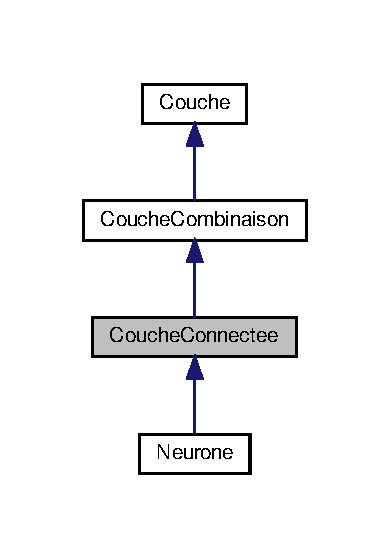
\includegraphics[width=187pt]{class_couche_connectee__inherit__graph}
\end{center}
\end{figure}


Graphe de collaboration de Couche\+Connectee\+:\nopagebreak
\begin{figure}[H]
\begin{center}
\leavevmode
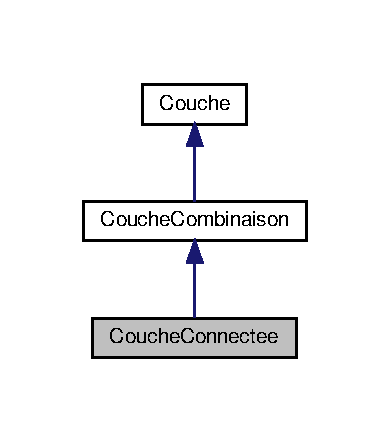
\includegraphics[width=187pt]{class_couche_connectee__coll__graph}
\end{center}
\end{figure}
\subsection*{Fonctions membres publiques}
\begin{DoxyCompactItemize}
\item 
\mbox{\Hypertarget{class_couche_connectee_a57bb158c3d73fc0b19cc44cdc2946e0d}\label{class_couche_connectee_a57bb158c3d73fc0b19cc44cdc2946e0d}} 
\hyperlink{class_couche_connectee_a57bb158c3d73fc0b19cc44cdc2946e0d}{Couche\+Connectee} (\hyperlink{class_dim_tenseur}{Dim\+Tenseur} din, \hyperlink{class_dim_tenseur}{Dim\+Tenseur} dout, std\+::string no, \hyperlink{class_tenseur}{Tenseur} par)
\begin{DoxyCompactList}\small\item\em Constructeur d\textquotesingle{}une couche connectée à partir du nombre de sorties. \end{DoxyCompactList}\item 
\hyperlink{class_tenseur}{Tenseur} \hyperlink{class_couche_connectee_acd60c499c6c74f914795f45f3f8084d0}{propagation} (\hyperlink{class_tenseur}{Tenseur} t)
\begin{DoxyCompactList}\small\item\em Methode permettant la propagation d\textquotesingle{}une couche à une autre. \end{DoxyCompactList}\end{DoxyCompactItemize}


\subsection{Description détaillée}


Définition à la ligne 17 du fichier Couche\+Connectee.\+hpp.



\subsection{Documentation des fonctions membres}
\mbox{\Hypertarget{class_couche_connectee_acd60c499c6c74f914795f45f3f8084d0}\label{class_couche_connectee_acd60c499c6c74f914795f45f3f8084d0}} 
\index{Couche\+Connectee@{Couche\+Connectee}!propagation@{propagation}}
\index{propagation@{propagation}!Couche\+Connectee@{Couche\+Connectee}}
\subsubsection{\texorpdfstring{propagation()}{propagation()}}
{\footnotesize\ttfamily \hyperlink{class_tenseur}{Tenseur} Couche\+Connectee\+::propagation (\begin{DoxyParamCaption}\item[{\hyperlink{class_tenseur}{Tenseur}}]{t }\end{DoxyParamCaption})\hspace{0.3cm}{\ttfamily [virtual]}}



Methode permettant la propagation d\textquotesingle{}une couche à une autre. 


\begin{DoxyParams}{Paramètres}
{\em t} & le tenseur d\textquotesingle{}entree \\
\hline
\end{DoxyParams}
\begin{DoxyReturn}{Renvoie}
la sortie de la couche 
\end{DoxyReturn}


Réimplémentée à partir de \hyperlink{class_couche_a1f0ed59e21020f5d4f37933af4d1b1e5}{Couche}.



Définition à la ligne 8 du fichier Couche\+Connectee.\+cpp.



La documentation de cette classe a été générée à partir des fichiers suivants \+:\begin{DoxyCompactItemize}
\item 
src/deeplearn/archi/Couche\+Connectee.\+hpp\item 
src/deeplearn/archi/Couche\+Connectee.\+cpp\end{DoxyCompactItemize}

\hypertarget{class_couche_connect_xC3_xA9e}{}\section{Référence de la classe Couche\+Connectée}
\label{class_couche_connect_xC3_xA9e}\index{Couche\+Connectée@{Couche\+Connectée}}


Création d\textquotesingle{}une couche connectee.  




{\ttfamily \#include $<$Couche\+Connectee.\+hpp$>$}



\subsection{Description détaillée}
Création d\textquotesingle{}une couche connectee. 

Création d\textquotesingle{}un neurone.

\begin{DoxyAuthor}{Auteur}
Adrien 
\end{DoxyAuthor}
\begin{DoxyVersion}{Version}
1.\+0 
\end{DoxyVersion}
\begin{DoxyDate}{Date}
avril 2019
\end{DoxyDate}
Classe permettant la création d\textquotesingle{}une couche de combinaison de \char`\"{}type\char`\"{} connectée \+: tous les neurones sont reliés d\textquotesingle{}une couche à une autre.

\begin{DoxyAuthor}{Auteur}
Adrien 
\end{DoxyAuthor}
\begin{DoxyVersion}{Version}
1.\+0 
\end{DoxyVersion}
\begin{DoxyDate}{Date}
avril 2019
\end{DoxyDate}
Classe permettant la création d\textquotesingle{}un neurone. Cette classe hérite de la classe \hyperlink{class_couche_connect_xC3_xA9e}{Couche\+Connectée}. 

La documentation de cette classe a été générée à partir du fichier suivant \+:\begin{DoxyCompactItemize}
\item 
src/deeplearn/archi/Couche\+Connectee.\+hpp\end{DoxyCompactItemize}

\hypertarget{class_couche_convolutive}{}\section{Référence de la classe Couche\+Convolutive}
\label{class_couche_convolutive}\index{Couche\+Convolutive@{Couche\+Convolutive}}


Création d\textquotesingle{}une couche convolutive.  




{\ttfamily \#include $<$Couche\+Convolutive.\+hpp$>$}



Graphe d\textquotesingle{}héritage de Couche\+Convolutive\+:\nopagebreak
\begin{figure}[H]
\begin{center}
\leavevmode
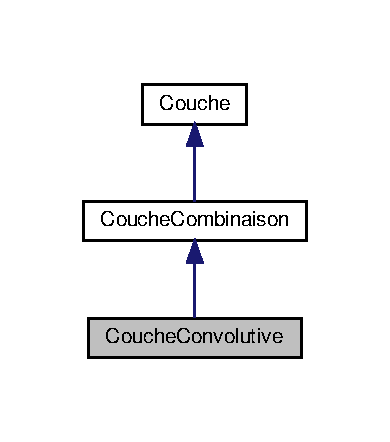
\includegraphics[width=187pt]{class_couche_convolutive__inherit__graph}
\end{center}
\end{figure}


Graphe de collaboration de Couche\+Convolutive\+:\nopagebreak
\begin{figure}[H]
\begin{center}
\leavevmode
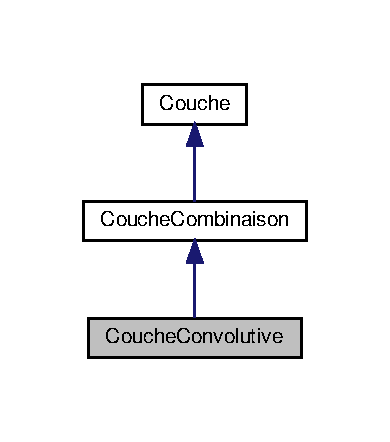
\includegraphics[width=187pt]{class_couche_convolutive__coll__graph}
\end{center}
\end{figure}
\subsection*{Fonctions membres publiques}
\begin{DoxyCompactItemize}
\item 
\hyperlink{class_couche_convolutive_ac0e9fc1269646ff46ab9ea2a26489123}{Couche\+Convolutive} (\hyperlink{class_dim_tenseur}{Dim\+Tenseur} din, \hyperlink{class_dim_tenseur}{Dim\+Tenseur} dout, std\+::string no, \hyperlink{class_tenseur}{Tenseur} par, int l\+\_\+fil, int h\+\_\+fil, int nb\+\_\+fil)
\begin{DoxyCompactList}\small\item\em Constructeur d\textquotesingle{}une couche convolutive à partir de la longeur du filtre, de la hauteur du filtre et du nombre de filtres. \end{DoxyCompactList}\item 
\hyperlink{class_tenseur}{Tenseur} \hyperlink{class_couche_convolutive_ad1a55b3dc9bf52e0725ae2a7b2e92aa1}{propagation} (\hyperlink{class_tenseur}{Tenseur} t)
\begin{DoxyCompactList}\small\item\em Méthode permettant la propagation d\textquotesingle{}une couche a une autre. \end{DoxyCompactList}\item 
\mbox{\Hypertarget{class_couche_convolutive_a1923173423085bc194b2484ff7b6d922}\label{class_couche_convolutive_a1923173423085bc194b2484ff7b6d922}} 
void \hyperlink{class_couche_convolutive_a1923173423085bc194b2484ff7b6d922}{set\+L\+\_\+\+Filtre} (int l\+\_\+fil)
\begin{DoxyCompactList}\small\item\em Changer la longueur de chaque filtre. \end{DoxyCompactList}\item 
\mbox{\Hypertarget{class_couche_convolutive_a352b530060db1a2b20a8df3f9daaf026}\label{class_couche_convolutive_a352b530060db1a2b20a8df3f9daaf026}} 
void {\bfseries set\+H\+\_\+\+Filtre} (int h\+\_\+fil)
\item 
void \hyperlink{class_couche_convolutive_a30fd844fc3a96f2e90d1a20251b1bfe3}{set\+Params} (int nb\+\_\+filtres)
\begin{DoxyCompactList}\small\item\em Changer la largeur de chaque filtre. \end{DoxyCompactList}\end{DoxyCompactItemize}


\subsection{Description détaillée}
Création d\textquotesingle{}une couche convolutive. 

\begin{DoxyAuthor}{Auteur}
Adrien 
\end{DoxyAuthor}
\begin{DoxyVersion}{Version}
1.\+0 
\end{DoxyVersion}
\begin{DoxyDate}{Date}
avril 2019
\end{DoxyDate}
Classe permettant la création d\textquotesingle{}une couche de combinaison de \char`\"{}type\char`\"{} convolutive. 

Définition à la ligne 17 du fichier Couche\+Convolutive.\+hpp.



\subsection{Documentation des constructeurs et destructeur}
\mbox{\Hypertarget{class_couche_convolutive_ac0e9fc1269646ff46ab9ea2a26489123}\label{class_couche_convolutive_ac0e9fc1269646ff46ab9ea2a26489123}} 
\index{Couche\+Convolutive@{Couche\+Convolutive}!Couche\+Convolutive@{Couche\+Convolutive}}
\index{Couche\+Convolutive@{Couche\+Convolutive}!Couche\+Convolutive@{Couche\+Convolutive}}
\subsubsection{\texorpdfstring{Couche\+Convolutive()}{CoucheConvolutive()}}
{\footnotesize\ttfamily Couche\+Convolutive\+::\+Couche\+Convolutive (\begin{DoxyParamCaption}\item[{\hyperlink{class_dim_tenseur}{Dim\+Tenseur}}]{din,  }\item[{\hyperlink{class_dim_tenseur}{Dim\+Tenseur}}]{dout,  }\item[{std\+::string}]{no,  }\item[{\hyperlink{class_tenseur}{Tenseur}}]{par,  }\item[{int}]{l\+\_\+fil,  }\item[{int}]{h\+\_\+fil,  }\item[{int}]{nb\+\_\+fil }\end{DoxyParamCaption})}



Constructeur d\textquotesingle{}une couche convolutive à partir de la longeur du filtre, de la hauteur du filtre et du nombre de filtres. 

Constructeur d\textquotesingle{}une couche convolutive à partir de la taille du tenseur d\textquotesingle{}entrée, de la longeur du filtre, de la hauteur du filtre et du nombre de $\ast$ filtres 

Définition à la ligne 3 du fichier Couche\+Convolutive.\+cpp.



\subsection{Documentation des fonctions membres}
\mbox{\Hypertarget{class_couche_convolutive_ad1a55b3dc9bf52e0725ae2a7b2e92aa1}\label{class_couche_convolutive_ad1a55b3dc9bf52e0725ae2a7b2e92aa1}} 
\index{Couche\+Convolutive@{Couche\+Convolutive}!propagation@{propagation}}
\index{propagation@{propagation}!Couche\+Convolutive@{Couche\+Convolutive}}
\subsubsection{\texorpdfstring{propagation()}{propagation()}}
{\footnotesize\ttfamily \hyperlink{class_tenseur}{Tenseur} Couche\+Convolutive\+::propagation (\begin{DoxyParamCaption}\item[{\hyperlink{class_tenseur}{Tenseur}}]{t }\end{DoxyParamCaption})\hspace{0.3cm}{\ttfamily [virtual]}}



Méthode permettant la propagation d\textquotesingle{}une couche a une autre. 


\begin{DoxyParams}{Paramètres}
{\em t} & le tenseur d\textquotesingle{}entree \\
\hline
\end{DoxyParams}
\begin{DoxyReturn}{Renvoie}
la sortie de la couche 
\end{DoxyReturn}


Réimplémentée à partir de \hyperlink{class_couche_a1f0ed59e21020f5d4f37933af4d1b1e5}{Couche}.



Définition à la ligne 9 du fichier Couche\+Convolutive.\+cpp.

\mbox{\Hypertarget{class_couche_convolutive_a30fd844fc3a96f2e90d1a20251b1bfe3}\label{class_couche_convolutive_a30fd844fc3a96f2e90d1a20251b1bfe3}} 
\index{Couche\+Convolutive@{Couche\+Convolutive}!set\+Params@{set\+Params}}
\index{set\+Params@{set\+Params}!Couche\+Convolutive@{Couche\+Convolutive}}
\subsubsection{\texorpdfstring{set\+Params()}{setParams()}}
{\footnotesize\ttfamily void Couche\+Convolutive\+::set\+Params (\begin{DoxyParamCaption}\item[{int}]{nb\+\_\+filtres }\end{DoxyParamCaption})}



Changer la largeur de chaque filtre. 

Changer le nombre de filtres. 

La documentation de cette classe a été générée à partir des fichiers suivants \+:\begin{DoxyCompactItemize}
\item 
src/deeplearn/archi/Couche\+Convolutive.\+hpp\item 
src/deeplearn/archi/Couche\+Convolutive.\+cpp\end{DoxyCompactItemize}

\hypertarget{class_dim_tenseur}{}\section{Référence de la classe Dim\+Tenseur}
\label{class_dim_tenseur}\index{Dim\+Tenseur@{Dim\+Tenseur}}


Classe stockant les dimensions d\textquotesingle{}un tenseur.  




{\ttfamily \#include $<$Dim\+Tenseur.\+hpp$>$}

\subsection*{Fonctions membres publiques}
\begin{DoxyCompactItemize}
\item 
\mbox{\Hypertarget{class_dim_tenseur_a599e42c7842cec590b226d3ac676933e}\label{class_dim_tenseur_a599e42c7842cec590b226d3ac676933e}} 
\hyperlink{class_dim_tenseur_a599e42c7842cec590b226d3ac676933e}{Dim\+Tenseur} ()
\begin{DoxyCompactList}\small\item\em Constructeur standard. \end{DoxyCompactList}\item 
\mbox{\Hypertarget{class_dim_tenseur_aa0faeff63ad7ca344ee327ec974001fe}\label{class_dim_tenseur_aa0faeff63ad7ca344ee327ec974001fe}} 
\hyperlink{class_dim_tenseur_aa0faeff63ad7ca344ee327ec974001fe}{Dim\+Tenseur} (int ord, std\+::vector$<$ int $>$ di)
\begin{DoxyCompactList}\small\item\em Constructeur avec d\textquotesingle{}obtenir la dimension souhaitée. \end{DoxyCompactList}\item 
int \hyperlink{class_dim_tenseur_a0d1e2833c775440baad2ac390cc6e135}{get\+Ordre} ()
\begin{DoxyCompactList}\small\item\em Méthode pour obtenir l\textquotesingle{}ordre du tenseur. \end{DoxyCompactList}\item 
std\+::vector$<$ int $>$ \hyperlink{class_dim_tenseur_a987995f83a0c8debb5f75edb59dad3b0}{get\+Dim} ()
\begin{DoxyCompactList}\small\item\em Méthode pour obtenir la liste des dimensions du tenseur. \end{DoxyCompactList}\end{DoxyCompactItemize}


\subsection{Description détaillée}
Classe stockant les dimensions d\textquotesingle{}un tenseur. 

\begin{DoxyAuthor}{Auteur}
Adrien 
\end{DoxyAuthor}
\begin{DoxyVersion}{Version}
1.\+0 
\end{DoxyVersion}
\begin{DoxyDate}{Date}
avril 2019
\end{DoxyDate}
Classe qui gère la dimension d\textquotesingle{}un tenseur 

Définition à la ligne 18 du fichier Dim\+Tenseur.\+hpp.



\subsection{Documentation des fonctions membres}
\mbox{\Hypertarget{class_dim_tenseur_a987995f83a0c8debb5f75edb59dad3b0}\label{class_dim_tenseur_a987995f83a0c8debb5f75edb59dad3b0}} 
\index{Dim\+Tenseur@{Dim\+Tenseur}!get\+Dim@{get\+Dim}}
\index{get\+Dim@{get\+Dim}!Dim\+Tenseur@{Dim\+Tenseur}}
\subsubsection{\texorpdfstring{get\+Dim()}{getDim()}}
{\footnotesize\ttfamily \hyperlink{class_dim_tenseur}{Dim\+Tenseur} Dim\+Tenseur\+::get\+Dim (\begin{DoxyParamCaption}{ }\end{DoxyParamCaption})}



Méthode pour obtenir la liste des dimensions du tenseur. 

\begin{DoxyReturn}{Renvoie}
la liste des dimensions du tenseur 
\end{DoxyReturn}


Définition à la ligne 26 du fichier Dim\+Tenseur.\+cpp.

\mbox{\Hypertarget{class_dim_tenseur_a0d1e2833c775440baad2ac390cc6e135}\label{class_dim_tenseur_a0d1e2833c775440baad2ac390cc6e135}} 
\index{Dim\+Tenseur@{Dim\+Tenseur}!get\+Ordre@{get\+Ordre}}
\index{get\+Ordre@{get\+Ordre}!Dim\+Tenseur@{Dim\+Tenseur}}
\subsubsection{\texorpdfstring{get\+Ordre()}{getOrdre()}}
{\footnotesize\ttfamily int Dim\+Tenseur\+::get\+Ordre (\begin{DoxyParamCaption}{ }\end{DoxyParamCaption})}



Méthode pour obtenir l\textquotesingle{}ordre du tenseur. 

\begin{DoxyReturn}{Renvoie}
l\textquotesingle{}ordre du tenseur 
\end{DoxyReturn}


Définition à la ligne 19 du fichier Dim\+Tenseur.\+cpp.



La documentation de cette classe a été générée à partir des fichiers suivants \+:\begin{DoxyCompactItemize}
\item 
src/deeplearn/archi/Dim\+Tenseur.\+hpp\item 
src/deeplearn/archi/Dim\+Tenseur.\+cpp\end{DoxyCompactItemize}

\hypertarget{class_donnee}{}\section{Référence de la classe Donnee}
\label{class_donnee}\index{Donnee@{Donnee}}


Gère une des donnees necessaires a l\textquotesingle{}apprentissage.  




{\ttfamily \#include $<$Donnee.\+hpp$>$}

\subsection*{Fonctions membres publiques}
\begin{DoxyCompactItemize}
\item 
\mbox{\Hypertarget{class_donnee_a41bbb1e9a6835479eefa2a694ddd5da3}\label{class_donnee_a41bbb1e9a6835479eefa2a694ddd5da3}} 
\hyperlink{class_donnee_a41bbb1e9a6835479eefa2a694ddd5da3}{Donnee} (\hyperlink{class_tenseur}{Tenseur} entree, \hyperlink{class_tenseur}{Tenseur} sortie)
\begin{DoxyCompactList}\small\item\em Constructeur de \hyperlink{class_donnee}{Donnee} avec une entree et une sortie. \end{DoxyCompactList}\item 
\hyperlink{class_tenseur}{Tenseur} \hyperlink{class_donnee_af4b02bb80cd289073f1eb56fc9046c11}{get\+Entree} ()
\begin{DoxyCompactList}\small\item\em Retourne l\textquotesingle{}entree de la donnee. \end{DoxyCompactList}\item 
\hyperlink{class_tenseur}{Tenseur} \hyperlink{class_donnee_aadc9c0ab3f163fa6c0e57daa57023de0}{get\+Sortie} ()
\begin{DoxyCompactList}\small\item\em Retourne la sortie de la donnee. \end{DoxyCompactList}\item 
void \hyperlink{class_donnee_ad8f000cbd829b3f3485cc158b5a92514}{set\+Entree} (\hyperlink{class_tenseur}{Tenseur} e)
\begin{DoxyCompactList}\small\item\em Met a jour l\textquotesingle{}entree de la donnee. \end{DoxyCompactList}\item 
void \hyperlink{class_donnee_adbcb8dc22a69b7c0fffca3dbbef4623b}{set\+Sortie} (\hyperlink{class_tenseur}{Tenseur} s)
\begin{DoxyCompactList}\small\item\em Met a jour la sortie de la donnee. \end{DoxyCompactList}\end{DoxyCompactItemize}


\subsection{Description détaillée}
Gère une des donnees necessaires a l\textquotesingle{}apprentissage. 

\begin{DoxyAuthor}{Auteur}
Marion 
\end{DoxyAuthor}
\begin{DoxyVersion}{Version}
1.\+0 
\end{DoxyVersion}
\begin{DoxyDate}{Date}
avril 2019
\end{DoxyDate}
Module permettant le stockage en mémoire vive d\textquotesingle{}une donnee necessaire a l\textquotesingle{}apprentissage. La donnee est vu comme un couple Entree/\+Sortie. 

Définition à la ligne 17 du fichier Donnee.\+hpp.



\subsection{Documentation des fonctions membres}
\mbox{\Hypertarget{class_donnee_af4b02bb80cd289073f1eb56fc9046c11}\label{class_donnee_af4b02bb80cd289073f1eb56fc9046c11}} 
\index{Donnee@{Donnee}!get\+Entree@{get\+Entree}}
\index{get\+Entree@{get\+Entree}!Donnee@{Donnee}}
\subsubsection{\texorpdfstring{get\+Entree()}{getEntree()}}
{\footnotesize\ttfamily \hyperlink{class_tenseur}{Tenseur} Donnee\+::get\+Entree (\begin{DoxyParamCaption}{ }\end{DoxyParamCaption})}



Retourne l\textquotesingle{}entree de la donnee. 

\begin{DoxyReturn}{Renvoie}
l\textquotesingle{}entree. $\ast$ 
\end{DoxyReturn}
\mbox{\Hypertarget{class_donnee_aadc9c0ab3f163fa6c0e57daa57023de0}\label{class_donnee_aadc9c0ab3f163fa6c0e57daa57023de0}} 
\index{Donnee@{Donnee}!get\+Sortie@{get\+Sortie}}
\index{get\+Sortie@{get\+Sortie}!Donnee@{Donnee}}
\subsubsection{\texorpdfstring{get\+Sortie()}{getSortie()}}
{\footnotesize\ttfamily \hyperlink{class_tenseur}{Tenseur} Donnee\+::get\+Sortie (\begin{DoxyParamCaption}{ }\end{DoxyParamCaption})}



Retourne la sortie de la donnee. 

\begin{DoxyReturn}{Renvoie}
la sortie. $\ast$ $\ast$ 
\end{DoxyReturn}
\mbox{\Hypertarget{class_donnee_ad8f000cbd829b3f3485cc158b5a92514}\label{class_donnee_ad8f000cbd829b3f3485cc158b5a92514}} 
\index{Donnee@{Donnee}!set\+Entree@{set\+Entree}}
\index{set\+Entree@{set\+Entree}!Donnee@{Donnee}}
\subsubsection{\texorpdfstring{set\+Entree()}{setEntree()}}
{\footnotesize\ttfamily void Donnee\+::set\+Entree (\begin{DoxyParamCaption}\item[{\hyperlink{class_tenseur}{Tenseur}}]{e }\end{DoxyParamCaption})}



Met a jour l\textquotesingle{}entree de la donnee. 


\begin{DoxyParams}{Paramètres}
{\em e} & le tenseur d\textquotesingle{}entree \\
\hline
\end{DoxyParams}
\mbox{\Hypertarget{class_donnee_adbcb8dc22a69b7c0fffca3dbbef4623b}\label{class_donnee_adbcb8dc22a69b7c0fffca3dbbef4623b}} 
\index{Donnee@{Donnee}!set\+Sortie@{set\+Sortie}}
\index{set\+Sortie@{set\+Sortie}!Donnee@{Donnee}}
\subsubsection{\texorpdfstring{set\+Sortie()}{setSortie()}}
{\footnotesize\ttfamily void Donnee\+::set\+Sortie (\begin{DoxyParamCaption}\item[{\hyperlink{class_tenseur}{Tenseur}}]{s }\end{DoxyParamCaption})}



Met a jour la sortie de la donnee. 


\begin{DoxyParams}{Paramètres}
{\em s} & le tenseur de sortie \\
\hline
\end{DoxyParams}


La documentation de cette classe a été générée à partir du fichier suivant \+:\begin{DoxyCompactItemize}
\item 
src/deeplearn/train/Donnee.\+hpp\end{DoxyCompactItemize}

\hypertarget{class_donnees}{}\section{Référence de la classe Donnees}
\label{class_donnees}\index{Donnees@{Donnees}}


Gère les donnees necessaire a l\textquotesingle{}apprentissage.  




{\ttfamily \#include $<$Donnees.\+hpp$>$}

\subsection*{Fonctions membres publiques}
\begin{DoxyCompactItemize}
\item 
\mbox{\Hypertarget{class_donnees_af6379b2712677e845cf58e37000f9b75}\label{class_donnees_af6379b2712677e845cf58e37000f9b75}} 
\hyperlink{class_donnees_af6379b2712677e845cf58e37000f9b75}{Donnees} ()
\begin{DoxyCompactList}\small\item\em Constructeur des donnees d\textquotesingle{}apprentissage. \end{DoxyCompactList}\item 
\mbox{\Hypertarget{class_donnees_aab4dadccfdee90d79faedaa42a3200b8}\label{class_donnees_aab4dadccfdee90d79faedaa42a3200b8}} 
\hyperlink{class_donnees_aab4dadccfdee90d79faedaa42a3200b8}{Donnees} (std\+::vector$<$ \hyperlink{class_donnee}{Donnee} $>$ vd)
\begin{DoxyCompactList}\small\item\em Constructeur des donnees d\textquotesingle{}apprentissage a partir d\textquotesingle{}un vecteur de donnees unitaires. \end{DoxyCompactList}\item 
void \hyperlink{class_donnees_a26d282aff1a7adfdcaea1a3cab6ffbaf}{ajouter\+Donnees} (\hyperlink{class_donnees}{Donnees} d)
\begin{DoxyCompactList}\small\item\em Ajoute un ensemble de donnees. \end{DoxyCompactList}\item 
void \hyperlink{class_donnees_a7f77ebe53ea55a3293cefb864d60e7ff}{ajouter\+Donnee} (\hyperlink{class_donnee}{Donnee} d)
\begin{DoxyCompactList}\small\item\em Ajoute une donnee a l\textquotesingle{}ensemble des donnees. \end{DoxyCompactList}\item 
\mbox{\Hypertarget{class_donnees_a722ba74b5e8c6bc0a2f7c16589692ad5}\label{class_donnees_a722ba74b5e8c6bc0a2f7c16589692ad5}} 
void \hyperlink{class_donnees_a722ba74b5e8c6bc0a2f7c16589692ad5}{melanger} ()
\begin{DoxyCompactList}\small\item\em Melange les donnees. \end{DoxyCompactList}\item 
\hyperlink{class_donnee}{Donnee} \hyperlink{class_donnees_a1986c4b95b3cf90767dbe966b2497ae8}{get\+Donnee} (int num)
\begin{DoxyCompactList}\small\item\em Retourne la donnee numero num parmis l\textquotesingle{}ensemble des donnees. \end{DoxyCompactList}\item 
std\+::vector$<$ \hyperlink{class_donnees}{Donnees} $>$ \hyperlink{class_donnees_acb2f30978cb824d70c39b716c49fe1fa}{get\+Donnees} ()
\begin{DoxyCompactList}\small\item\em Retourne l\textquotesingle{}ensemble des donnees. \end{DoxyCompactList}\item 
int \hyperlink{class_donnees_a4c4da37884b1b91d881524f2a7b91dbc}{get\+Nb\+Donnees} ()
\begin{DoxyCompactList}\small\item\em Retourne le nombre de donnees. \end{DoxyCompactList}\end{DoxyCompactItemize}


\subsection{Description détaillée}
Gère les donnees necessaire a l\textquotesingle{}apprentissage. 

\begin{DoxyAuthor}{Auteur}
Marion 
\end{DoxyAuthor}
\begin{DoxyVersion}{Version}
1.\+0 
\end{DoxyVersion}
\begin{DoxyDate}{Date}
avril 2019
\end{DoxyDate}
Module permettant le stockage en memoire vive des donnees necessaire a l\textquotesingle{}apprentissage. 

Définition à la ligne 18 du fichier Donnees.\+hpp.



\subsection{Documentation des fonctions membres}
\mbox{\Hypertarget{class_donnees_a7f77ebe53ea55a3293cefb864d60e7ff}\label{class_donnees_a7f77ebe53ea55a3293cefb864d60e7ff}} 
\index{Donnees@{Donnees}!ajouter\+Donnee@{ajouter\+Donnee}}
\index{ajouter\+Donnee@{ajouter\+Donnee}!Donnees@{Donnees}}
\subsubsection{\texorpdfstring{ajouter\+Donnee()}{ajouterDonnee()}}
{\footnotesize\ttfamily void Donnees\+::ajouter\+Donnee (\begin{DoxyParamCaption}\item[{\hyperlink{class_donnee}{Donnee}}]{d }\end{DoxyParamCaption})}



Ajoute une donnee a l\textquotesingle{}ensemble des donnees. 


\begin{DoxyParams}{Paramètres}
{\em d} & la donnee a ajouter \\
\hline
\end{DoxyParams}
\mbox{\Hypertarget{class_donnees_a26d282aff1a7adfdcaea1a3cab6ffbaf}\label{class_donnees_a26d282aff1a7adfdcaea1a3cab6ffbaf}} 
\index{Donnees@{Donnees}!ajouter\+Donnees@{ajouter\+Donnees}}
\index{ajouter\+Donnees@{ajouter\+Donnees}!Donnees@{Donnees}}
\subsubsection{\texorpdfstring{ajouter\+Donnees()}{ajouterDonnees()}}
{\footnotesize\ttfamily void Donnees\+::ajouter\+Donnees (\begin{DoxyParamCaption}\item[{\hyperlink{class_donnees}{Donnees}}]{d }\end{DoxyParamCaption})}



Ajoute un ensemble de donnees. 


\begin{DoxyParams}{Paramètres}
{\em d} & l\textquotesingle{}ensemble des donnees \\
\hline
\end{DoxyParams}
\mbox{\Hypertarget{class_donnees_a1986c4b95b3cf90767dbe966b2497ae8}\label{class_donnees_a1986c4b95b3cf90767dbe966b2497ae8}} 
\index{Donnees@{Donnees}!get\+Donnee@{get\+Donnee}}
\index{get\+Donnee@{get\+Donnee}!Donnees@{Donnees}}
\subsubsection{\texorpdfstring{get\+Donnee()}{getDonnee()}}
{\footnotesize\ttfamily \hyperlink{class_donnee}{Donnee} Donnees\+::get\+Donnee (\begin{DoxyParamCaption}\item[{int}]{num }\end{DoxyParamCaption})}



Retourne la donnee numero num parmis l\textquotesingle{}ensemble des donnees. 


\begin{DoxyParams}{Paramètres}
{\em num} & le numero de la donnee \\
\hline
\end{DoxyParams}
\begin{DoxyReturn}{Renvoie}
la donnee en position \char`\"{}num\char`\"{} 
\end{DoxyReturn}
\mbox{\Hypertarget{class_donnees_acb2f30978cb824d70c39b716c49fe1fa}\label{class_donnees_acb2f30978cb824d70c39b716c49fe1fa}} 
\index{Donnees@{Donnees}!get\+Donnees@{get\+Donnees}}
\index{get\+Donnees@{get\+Donnees}!Donnees@{Donnees}}
\subsubsection{\texorpdfstring{get\+Donnees()}{getDonnees()}}
{\footnotesize\ttfamily vector$<$ \hyperlink{class_donnees}{Donnees} $>$ Donnees\+::get\+Donnees (\begin{DoxyParamCaption}{ }\end{DoxyParamCaption})}



Retourne l\textquotesingle{}ensemble des donnees. 

\begin{DoxyReturn}{Renvoie}
le vecteur des donnees 
\end{DoxyReturn}
\mbox{\Hypertarget{class_donnees_a4c4da37884b1b91d881524f2a7b91dbc}\label{class_donnees_a4c4da37884b1b91d881524f2a7b91dbc}} 
\index{Donnees@{Donnees}!get\+Nb\+Donnees@{get\+Nb\+Donnees}}
\index{get\+Nb\+Donnees@{get\+Nb\+Donnees}!Donnees@{Donnees}}
\subsubsection{\texorpdfstring{get\+Nb\+Donnees()}{getNbDonnees()}}
{\footnotesize\ttfamily int Donnees\+::get\+Nb\+Donnees (\begin{DoxyParamCaption}{ }\end{DoxyParamCaption})}



Retourne le nombre de donnees. 

\begin{DoxyReturn}{Renvoie}
le nombre de donnees 
\end{DoxyReturn}


La documentation de cette classe a été générée à partir du fichier suivant \+:\begin{DoxyCompactItemize}
\item 
src/deeplearn/train/Donnees.\+hpp\end{DoxyCompactItemize}

\hypertarget{class_erreur}{}\section{Référence de la classe Erreur}
\label{class_erreur}\index{Erreur@{Erreur}}


Gère le calcul de l\textquotesingle{}erreur commise lors d\textquotesingle{}un apprentissage.  




{\ttfamily \#include $<$Erreur.\+hpp$>$}



Graphe d\textquotesingle{}héritage de Erreur\+:\nopagebreak
\begin{figure}[H]
\begin{center}
\leavevmode
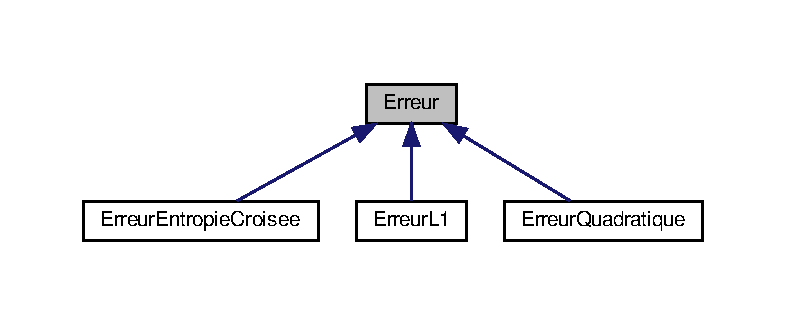
\includegraphics[width=350pt]{class_erreur__inherit__graph}
\end{center}
\end{figure}
\subsection*{Fonctions membres publiques}
\begin{DoxyCompactItemize}
\item 
virtual \hyperlink{class_tenseur}{Tenseur} \hyperlink{class_erreur_a0def45df23074388e2a338145aeb4660}{eval} (\hyperlink{class_tenseur}{Tenseur} sortie\+RN, \hyperlink{class_tenseur}{Tenseur} label)
\begin{DoxyCompactList}\small\item\em Methode virtuelle pour evaluer l\textquotesingle{}erreur effectuee entre la sortie et la prediction. \end{DoxyCompactList}\item 
virtual \hyperlink{class_tenseur}{Tenseur} \hyperlink{class_erreur_ad56634307e3ceb8ab5c2fddede28422a}{derivee} (\hyperlink{class_tenseur}{Tenseur} t)
\begin{DoxyCompactList}\small\item\em Méthode virtuelle pour avoir la derivee d\textquotesingle{}un tenseur donnee en entree. \end{DoxyCompactList}\end{DoxyCompactItemize}


\subsection{Description détaillée}
Gère le calcul de l\textquotesingle{}erreur commise lors d\textquotesingle{}un apprentissage. 

\begin{DoxyAuthor}{Auteur}
Marion 
\end{DoxyAuthor}
\begin{DoxyVersion}{Version}
1.\+0 
\end{DoxyVersion}
\begin{DoxyDate}{Date}
avril 2019
\end{DoxyDate}
Module permettant le traitement de l\textquotesingle{}erreur commise lors d\textquotesingle{}un apprentissage. Il permet également la récupération des données liées aux erreurs. 

Définition à la ligne 18 du fichier Erreur.\+hpp.



\subsection{Documentation des fonctions membres}
\mbox{\Hypertarget{class_erreur_ad56634307e3ceb8ab5c2fddede28422a}\label{class_erreur_ad56634307e3ceb8ab5c2fddede28422a}} 
\index{Erreur@{Erreur}!derivee@{derivee}}
\index{derivee@{derivee}!Erreur@{Erreur}}
\subsubsection{\texorpdfstring{derivee()}{derivee()}}
{\footnotesize\ttfamily void Erreur\+::derivee (\begin{DoxyParamCaption}\item[{\hyperlink{class_tenseur}{Tenseur}}]{t }\end{DoxyParamCaption})\hspace{0.3cm}{\ttfamily [virtual]}}



Méthode virtuelle pour avoir la derivee d\textquotesingle{}un tenseur donnee en entree. 


\begin{DoxyParams}{Paramètres}
{\em t} & le tenseur pour lequel on veut la derivee \\
\hline
\end{DoxyParams}
\mbox{\Hypertarget{class_erreur_a0def45df23074388e2a338145aeb4660}\label{class_erreur_a0def45df23074388e2a338145aeb4660}} 
\index{Erreur@{Erreur}!eval@{eval}}
\index{eval@{eval}!Erreur@{Erreur}}
\subsubsection{\texorpdfstring{eval()}{eval()}}
{\footnotesize\ttfamily \hyperlink{class_tenseur}{Tenseur} Erreur\+::eval (\begin{DoxyParamCaption}\item[{\hyperlink{class_tenseur}{Tenseur}}]{sortie\+RN,  }\item[{\hyperlink{class_tenseur}{Tenseur}}]{prediction }\end{DoxyParamCaption})\hspace{0.3cm}{\ttfamily [virtual]}}



Methode virtuelle pour evaluer l\textquotesingle{}erreur effectuee entre la sortie et la prediction. 


\begin{DoxyParams}{Paramètres}
{\em sortie\+RN} & le tenseur de sortie du reseau de neurones. \\
\hline
{\em label} & la sortie souhaitée du reseau de neurones. \\
\hline
\end{DoxyParams}


La documentation de cette classe a été générée à partir du fichier suivant \+:\begin{DoxyCompactItemize}
\item 
src/deeplearn/train/Erreur.\+hpp\end{DoxyCompactItemize}

\hypertarget{class_erreur_entropie_croisee}{}\section{Référence de la classe Erreur\+Entropie\+Croisee}
\label{class_erreur_entropie_croisee}\index{Erreur\+Entropie\+Croisee@{Erreur\+Entropie\+Croisee}}


Gère le calcul de l\textquotesingle{}erreur commise suivant l\textquotesingle{}entropie croisee lors d\textquotesingle{}un apprentissage.  




{\ttfamily \#include $<$Erreur\+Entropie\+Croisee.\+hpp$>$}



Graphe d\textquotesingle{}héritage de Erreur\+Entropie\+Croisee\+:\nopagebreak
\begin{figure}[H]
\begin{center}
\leavevmode
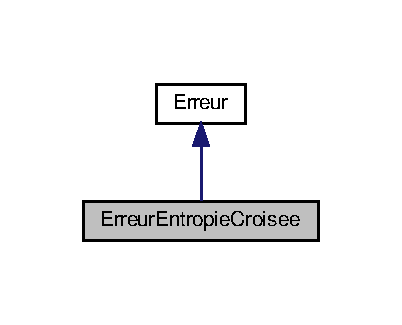
\includegraphics[width=193pt]{class_erreur_entropie_croisee__inherit__graph}
\end{center}
\end{figure}


Graphe de collaboration de Erreur\+Entropie\+Croisee\+:\nopagebreak
\begin{figure}[H]
\begin{center}
\leavevmode
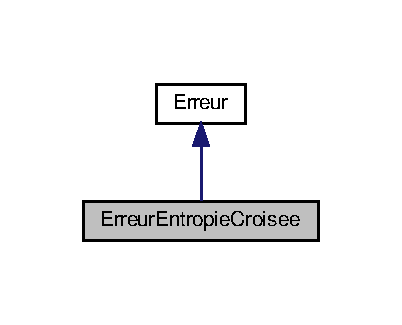
\includegraphics[width=193pt]{class_erreur_entropie_croisee__coll__graph}
\end{center}
\end{figure}
\subsection*{Fonctions membres publiques}
\begin{DoxyCompactItemize}
\item 
\mbox{\Hypertarget{class_erreur_entropie_croisee_ae79638c0e11e44100663e83f07273542}\label{class_erreur_entropie_croisee_ae79638c0e11e44100663e83f07273542}} 
\hyperlink{class_erreur_entropie_croisee_ae79638c0e11e44100663e83f07273542}{Erreur\+Entropie\+Croisee} ()
\begin{DoxyCompactList}\small\item\em Constructeur de l\textquotesingle{}erreur d\textquotesingle{}entropie croisee. \end{DoxyCompactList}\end{DoxyCompactItemize}


\subsection{Description détaillée}
Gère le calcul de l\textquotesingle{}erreur commise suivant l\textquotesingle{}entropie croisee lors d\textquotesingle{}un apprentissage. 

\begin{DoxyAuthor}{Auteur}
Marion 
\end{DoxyAuthor}
\begin{DoxyVersion}{Version}
1.\+0 
\end{DoxyVersion}
\begin{DoxyDate}{Date}
avril 2019
\end{DoxyDate}
Module permettant le traitement de l\textquotesingle{}erreur commise suivant l\textquotesingle{}entropie croisee lors d\textquotesingle{}un apprentissage. Il permet également la récupération des données liées aux erreurs. Il herite de la classe \hyperlink{class_erreur}{Erreur}. 

Définition à la ligne 19 du fichier Erreur\+Entropie\+Croisee.\+hpp.



La documentation de cette classe a été générée à partir du fichier suivant \+:\begin{DoxyCompactItemize}
\item 
src/deeplearn/train/Erreur\+Entropie\+Croisee.\+hpp\end{DoxyCompactItemize}

\hypertarget{class_erreur_l1}{}\section{Référence de la classe Erreur\+L1}
\label{class_erreur_l1}\index{Erreur\+L1@{Erreur\+L1}}


Gère le calcul de l\textquotesingle{}erreur commise lors d\textquotesingle{}un apprentissage suivant la norme L1.  




{\ttfamily \#include $<$Erreur\+L1.\+hpp$>$}



Graphe d\textquotesingle{}héritage de Erreur\+L1\+:\nopagebreak
\begin{figure}[H]
\begin{center}
\leavevmode
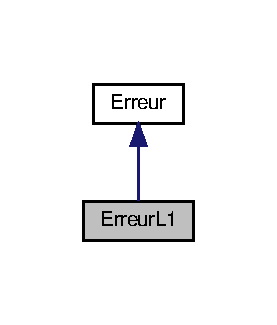
\includegraphics[width=133pt]{class_erreur_l1__inherit__graph}
\end{center}
\end{figure}


Graphe de collaboration de Erreur\+L1\+:\nopagebreak
\begin{figure}[H]
\begin{center}
\leavevmode
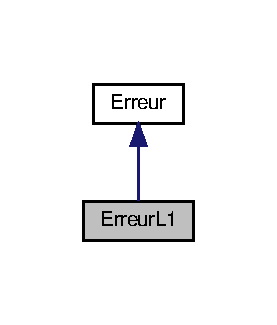
\includegraphics[width=133pt]{class_erreur_l1__coll__graph}
\end{center}
\end{figure}
\subsection*{Fonctions membres publiques}
\begin{DoxyCompactItemize}
\item 
\mbox{\Hypertarget{class_erreur_l1_ac22fa445742caeefafa848de6db282bf}\label{class_erreur_l1_ac22fa445742caeefafa848de6db282bf}} 
\hyperlink{class_erreur_l1_ac22fa445742caeefafa848de6db282bf}{Erreur\+L1} ()
\begin{DoxyCompactList}\small\item\em Constructeur de l\textquotesingle{}erreur L1. \end{DoxyCompactList}\end{DoxyCompactItemize}


\subsection{Description détaillée}
Gère le calcul de l\textquotesingle{}erreur commise lors d\textquotesingle{}un apprentissage suivant la norme L1. 

\begin{DoxyAuthor}{Auteur}
Marion 
\end{DoxyAuthor}
\begin{DoxyVersion}{Version}
1.\+0 
\end{DoxyVersion}
\begin{DoxyDate}{Date}
avril 2019
\end{DoxyDate}
Module permettant le traitement de l\textquotesingle{}erreur commise lors d\textquotesingle{}un apprentissage suivant la norme L1. Il permet également la récupération des données liées aux erreurs. Il herite de la classe \hyperlink{class_erreur}{Erreur}. 

Définition à la ligne 19 du fichier Erreur\+L1.\+hpp.



La documentation de cette classe a été générée à partir du fichier suivant \+:\begin{DoxyCompactItemize}
\item 
src/deeplearn/train/Erreur\+L1.\+hpp\end{DoxyCompactItemize}

\hypertarget{class_erreur_quadratique}{}\section{Référence de la classe Erreur\+Quadratique}
\label{class_erreur_quadratique}\index{Erreur\+Quadratique@{Erreur\+Quadratique}}


Gère le calcul de l\textquotesingle{}erreur commise de facon quadratique lors d\textquotesingle{}un apprentissage.  




{\ttfamily \#include $<$Erreur\+Quadratique.\+hpp$>$}



Graphe d\textquotesingle{}héritage de Erreur\+Quadratique\+:\nopagebreak
\begin{figure}[H]
\begin{center}
\leavevmode
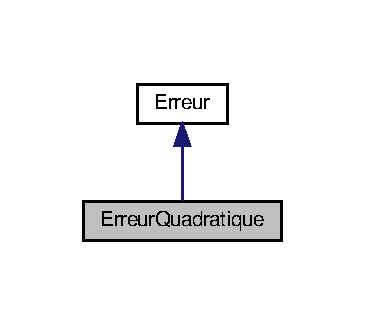
\includegraphics[width=175pt]{class_erreur_quadratique__inherit__graph}
\end{center}
\end{figure}


Graphe de collaboration de Erreur\+Quadratique\+:\nopagebreak
\begin{figure}[H]
\begin{center}
\leavevmode
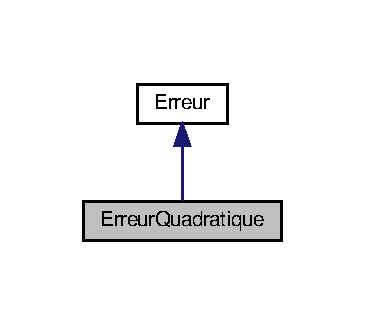
\includegraphics[width=175pt]{class_erreur_quadratique__coll__graph}
\end{center}
\end{figure}
\subsection*{Fonctions membres publiques}
\begin{DoxyCompactItemize}
\item 
\mbox{\Hypertarget{class_erreur_quadratique_aa11b896dc5e7ed5427568ee2c0bc1b1a}\label{class_erreur_quadratique_aa11b896dc5e7ed5427568ee2c0bc1b1a}} 
\hyperlink{class_erreur_quadratique_aa11b896dc5e7ed5427568ee2c0bc1b1a}{Erreur\+Quadratique} ()
\begin{DoxyCompactList}\small\item\em Constructeur de l\textquotesingle{}erreur quadratique. \end{DoxyCompactList}\end{DoxyCompactItemize}


\subsection{Description détaillée}
Gère le calcul de l\textquotesingle{}erreur commise de facon quadratique lors d\textquotesingle{}un apprentissage. 

\begin{DoxyAuthor}{Auteur}
Marion 
\end{DoxyAuthor}
\begin{DoxyVersion}{Version}
1.\+0 
\end{DoxyVersion}
\begin{DoxyDate}{Date}
avril 2019
\end{DoxyDate}
Module permettant le traitement de l\textquotesingle{}erreur quadratique commise lors d\textquotesingle{}un apprentissage. Il permet également la récupération des données liées aux erreurs. Il herite de la classe \hyperlink{class_erreur}{Erreur}. 

Définition à la ligne 19 du fichier Erreur\+Quadratique.\+hpp.



La documentation de cette classe a été générée à partir du fichier suivant \+:\begin{DoxyCompactItemize}
\item 
src/deeplearn/train/Erreur\+Quadratique.\+hpp\end{DoxyCompactItemize}

\hypertarget{class_graphe}{}\section{Référence du modèle de la classe Graphe$<$ Type $>$}
\label{class_graphe}\index{Graphe$<$ Type $>$@{Graphe$<$ Type $>$}}


Gestion du type \hyperlink{class_graphe}{Graphe}.  




{\ttfamily \#include $<$Graphe.\+hpp$>$}

\subsection*{Fonctions membres publiques}
\begin{DoxyCompactItemize}
\item 
\mbox{\Hypertarget{class_graphe_ac6269bd27d5bd9386348e34879619d2f}\label{class_graphe_ac6269bd27d5bd9386348e34879619d2f}} 
\hyperlink{class_graphe_ac6269bd27d5bd9386348e34879619d2f}{Graphe} ()
\begin{DoxyCompactList}\small\item\em Constructeur de graphe vide. \end{DoxyCompactList}\item 
\mbox{\Hypertarget{class_graphe_a4769b44ffb23da74a1b413857966c157}\label{class_graphe_a4769b44ffb23da74a1b413857966c157}} 
\hyperlink{class_graphe_a4769b44ffb23da74a1b413857966c157}{Graphe} (Type noeuds\mbox{[}$\,$\mbox{]})
\begin{DoxyCompactList}\small\item\em Constructeur de graphe à partir de noeuds isolés. \end{DoxyCompactList}\item 
void \hyperlink{class_graphe_a555829daa877e49cdb4e9555e559650c}{ajouter\+Noeud} (Type noeud)
\begin{DoxyCompactList}\small\item\em Ajout d\textquotesingle{}un noeud. \end{DoxyCompactList}\item 
void \hyperlink{class_graphe_a690a652df5be597b9045d2036bad11ed}{ajouter\+Arc} (Type noeud\+\_\+init, Type noeud\+\_\+final)
\begin{DoxyCompactList}\small\item\em Ajout d\textquotesingle{}un arc. \end{DoxyCompactList}\item 
void \hyperlink{class_graphe_a5887c7cd72bcf4b5f8c169a22b5180f1}{supprimer\+Noeud} (Type noeud)
\begin{DoxyCompactList}\small\item\em Suppression d\textquotesingle{}un noeud. \end{DoxyCompactList}\item 
void \hyperlink{class_graphe_a4d2b2b022f6c4747f15e1f4e059fef33}{supprimer\+Arc} (Type noeud\+\_\+init, Type noeud\+\_\+final)
\begin{DoxyCompactList}\small\item\em Suppression d\textquotesingle{}un arc. \end{DoxyCompactList}\item 
bool \hyperlink{class_graphe_aa003e00ed2d8c1d49c4b80e3dabfa4fd}{contient\+Cycle} ()
\begin{DoxyCompactList}\small\item\em Teste si le graphe contient un cycle. \end{DoxyCompactList}\item 
bool \hyperlink{class_graphe_a15609b3cd6e0ab6a96afb579ffd420c4}{est\+Connexe} ()
\begin{DoxyCompactList}\small\item\em Teste si le graphe est connexe. \end{DoxyCompactList}\end{DoxyCompactItemize}


\subsection{Description détaillée}
\subsubsection*{template$<$class Type$>$\newline
class Graphe$<$ Type $>$}

Gestion du type \hyperlink{class_graphe}{Graphe}. 


\begin{DoxyTemplParams}{Template Parameters}
{\em Type} & Type de noeud du graphe. \\
\hline
\end{DoxyTemplParams}
\begin{DoxyAuthor}{Auteur}
David 
\end{DoxyAuthor}
\begin{DoxyVersion}{Version}
1.\+0 
\end{DoxyVersion}
\begin{DoxyDate}{Date}
avril 2019
\end{DoxyDate}
Module permettant l\textquotesingle{}utilisation d\textquotesingle{}un graphe orienté générique. Les noeuds du graphe portent cette généricité et peuvent donc être de n\textquotesingle{}importe quel type de données. 

Définition à la ligne 19 du fichier Graphe.\+hpp.



\subsection{Documentation des fonctions membres}
\mbox{\Hypertarget{class_graphe_a690a652df5be597b9045d2036bad11ed}\label{class_graphe_a690a652df5be597b9045d2036bad11ed}} 
\index{Graphe@{Graphe}!ajouter\+Arc@{ajouter\+Arc}}
\index{ajouter\+Arc@{ajouter\+Arc}!Graphe@{Graphe}}
\subsubsection{\texorpdfstring{ajouter\+Arc()}{ajouterArc()}}
{\footnotesize\ttfamily template$<$class Type$>$ \\
void \hyperlink{class_graphe}{Graphe}$<$ Type $>$\+::ajouter\+Arc (\begin{DoxyParamCaption}\item[{Type}]{noeud\+\_\+init,  }\item[{Type}]{noeud\+\_\+final }\end{DoxyParamCaption})}



Ajout d\textquotesingle{}un arc. 


\begin{DoxyParams}{Paramètres}
{\em noeud\+\_\+init} & le noeud de départ de l\textquotesingle{}arc. \\
\hline
{\em noeud\+\_\+final} & le noeud d\textquotesingle{}arrivé de l\textquotesingle{}arc. \\
\hline
\end{DoxyParams}
\mbox{\Hypertarget{class_graphe_a555829daa877e49cdb4e9555e559650c}\label{class_graphe_a555829daa877e49cdb4e9555e559650c}} 
\index{Graphe@{Graphe}!ajouter\+Noeud@{ajouter\+Noeud}}
\index{ajouter\+Noeud@{ajouter\+Noeud}!Graphe@{Graphe}}
\subsubsection{\texorpdfstring{ajouter\+Noeud()}{ajouterNoeud()}}
{\footnotesize\ttfamily template$<$class Type$>$ \\
void \hyperlink{class_graphe}{Graphe}$<$ Type $>$\+::ajouter\+Noeud (\begin{DoxyParamCaption}\item[{Type}]{noeud }\end{DoxyParamCaption})}



Ajout d\textquotesingle{}un noeud. 


\begin{DoxyParams}{Paramètres}
{\em noeud} & un noeud du graphe. \\
\hline
\end{DoxyParams}
\mbox{\Hypertarget{class_graphe_aa003e00ed2d8c1d49c4b80e3dabfa4fd}\label{class_graphe_aa003e00ed2d8c1d49c4b80e3dabfa4fd}} 
\index{Graphe@{Graphe}!contient\+Cycle@{contient\+Cycle}}
\index{contient\+Cycle@{contient\+Cycle}!Graphe@{Graphe}}
\subsubsection{\texorpdfstring{contient\+Cycle()}{contientCycle()}}
{\footnotesize\ttfamily template$<$class Type$>$ \\
bool \hyperlink{class_graphe}{Graphe}$<$ Type $>$\+::contient\+Cycle (\begin{DoxyParamCaption}{ }\end{DoxyParamCaption})}



Teste si le graphe contient un cycle. 

\begin{DoxyReturn}{Renvoie}
un booléen. 
\end{DoxyReturn}
\mbox{\Hypertarget{class_graphe_a15609b3cd6e0ab6a96afb579ffd420c4}\label{class_graphe_a15609b3cd6e0ab6a96afb579ffd420c4}} 
\index{Graphe@{Graphe}!est\+Connexe@{est\+Connexe}}
\index{est\+Connexe@{est\+Connexe}!Graphe@{Graphe}}
\subsubsection{\texorpdfstring{est\+Connexe()}{estConnexe()}}
{\footnotesize\ttfamily template$<$class Type$>$ \\
bool \hyperlink{class_graphe}{Graphe}$<$ Type $>$\+::est\+Connexe (\begin{DoxyParamCaption}{ }\end{DoxyParamCaption})}



Teste si le graphe est connexe. 

\begin{DoxyReturn}{Renvoie}
un booléen. 
\end{DoxyReturn}
\mbox{\Hypertarget{class_graphe_a4d2b2b022f6c4747f15e1f4e059fef33}\label{class_graphe_a4d2b2b022f6c4747f15e1f4e059fef33}} 
\index{Graphe@{Graphe}!supprimer\+Arc@{supprimer\+Arc}}
\index{supprimer\+Arc@{supprimer\+Arc}!Graphe@{Graphe}}
\subsubsection{\texorpdfstring{supprimer\+Arc()}{supprimerArc()}}
{\footnotesize\ttfamily template$<$class Type$>$ \\
void \hyperlink{class_graphe}{Graphe}$<$ Type $>$\+::supprimer\+Arc (\begin{DoxyParamCaption}\item[{Type}]{noeud\+\_\+init,  }\item[{Type}]{noeud\+\_\+final }\end{DoxyParamCaption})}



Suppression d\textquotesingle{}un arc. 


\begin{DoxyParams}{Paramètres}
{\em noeud\+\_\+init} & le noeud de départ de l\textquotesingle{}arc. \\
\hline
{\em noeud\+\_\+final} & le noeud d\textquotesingle{}arrivé de l\textquotesingle{}arc. \\
\hline
\end{DoxyParams}
\mbox{\Hypertarget{class_graphe_a5887c7cd72bcf4b5f8c169a22b5180f1}\label{class_graphe_a5887c7cd72bcf4b5f8c169a22b5180f1}} 
\index{Graphe@{Graphe}!supprimer\+Noeud@{supprimer\+Noeud}}
\index{supprimer\+Noeud@{supprimer\+Noeud}!Graphe@{Graphe}}
\subsubsection{\texorpdfstring{supprimer\+Noeud()}{supprimerNoeud()}}
{\footnotesize\ttfamily template$<$class Type$>$ \\
void \hyperlink{class_graphe}{Graphe}$<$ Type $>$\+::supprimer\+Noeud (\begin{DoxyParamCaption}\item[{Type}]{noeud }\end{DoxyParamCaption})}



Suppression d\textquotesingle{}un noeud. 


\begin{DoxyParams}{Paramètres}
{\em noeud} & un noeud du graphe. \\
\hline
\end{DoxyParams}


La documentation de cette classe a été générée à partir du fichier suivant \+:\begin{DoxyCompactItemize}
\item 
src/deeplearn/archi/Graphe.\+hpp\end{DoxyCompactItemize}

\hypertarget{class_matrice}{}\section{Référence de la classe Matrice}
\label{class_matrice}\index{Matrice@{Matrice}}


Classe qui crée une matrice.  




{\ttfamily \#include $<$Matrice.\+hpp$>$}



Graphe d\textquotesingle{}héritage de Matrice\+:\nopagebreak
\begin{figure}[H]
\begin{center}
\leavevmode
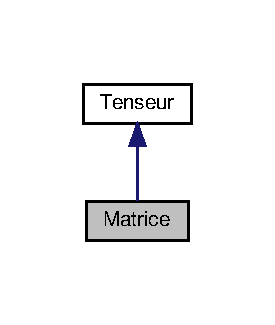
\includegraphics[width=132pt]{class_matrice__inherit__graph}
\end{center}
\end{figure}


Graphe de collaboration de Matrice\+:\nopagebreak
\begin{figure}[H]
\begin{center}
\leavevmode
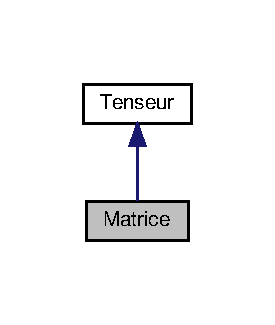
\includegraphics[width=132pt]{class_matrice__coll__graph}
\end{center}
\end{figure}
\subsection*{Fonctions membres publiques}
\begin{DoxyCompactItemize}
\item 
\mbox{\Hypertarget{class_matrice_aefac14911f8386860ddbac4c3a3c8812}\label{class_matrice_aefac14911f8386860ddbac4c3a3c8812}} 
\hyperlink{class_matrice_aefac14911f8386860ddbac4c3a3c8812}{Matrice} (void $\ast$valeur, int l, int c)
\begin{DoxyCompactList}\small\item\em Constructeur d\textquotesingle{}une matrice de taille lxc. \end{DoxyCompactList}\item 
\hyperlink{class_matrice}{Matrice} \hyperlink{class_matrice_a80ddaeb41cd4e71cd2edd13c206c109d}{produit\+Matriciel} (\hyperlink{class_matrice}{Matrice} m1)
\begin{DoxyCompactList}\small\item\em Méthode qui calcule le produit matriciel entre 2 matrices. \end{DoxyCompactList}\end{DoxyCompactItemize}


\subsection{Description détaillée}
Classe qui crée une matrice. 

\begin{DoxyAuthor}{Auteur}
Adrien 
\end{DoxyAuthor}
\begin{DoxyVersion}{Version}
1.\+0 
\end{DoxyVersion}
\begin{DoxyDate}{Date}
avril 2019
\end{DoxyDate}
Classe qui crée un tenseur d\textquotesingle{}ordre 2 (= matrice). 

Définition à la ligne 17 du fichier Matrice.\+hpp.



\subsection{Documentation des fonctions membres}
\mbox{\Hypertarget{class_matrice_a80ddaeb41cd4e71cd2edd13c206c109d}\label{class_matrice_a80ddaeb41cd4e71cd2edd13c206c109d}} 
\index{Matrice@{Matrice}!produit\+Matriciel@{produit\+Matriciel}}
\index{produit\+Matriciel@{produit\+Matriciel}!Matrice@{Matrice}}
\subsubsection{\texorpdfstring{produit\+Matriciel()}{produitMatriciel()}}
{\footnotesize\ttfamily \hyperlink{class_matrice}{Matrice} Matrice\+::produit\+Matriciel (\begin{DoxyParamCaption}\item[{\hyperlink{class_matrice}{Matrice}}]{m1 }\end{DoxyParamCaption})}



Méthode qui calcule le produit matriciel entre 2 matrices. 


\begin{DoxyParams}{Paramètres}
{\em une} & matrice \\
\hline
\end{DoxyParams}
\begin{DoxyReturn}{Renvoie}
une matrice 
\end{DoxyReturn}


La documentation de cette classe a été générée à partir des fichiers suivants \+:\begin{DoxyCompactItemize}
\item 
src/deeplearn/archi/Matrice.\+hpp\item 
src/deeplearn/archi/Matrice.\+cpp\end{DoxyCompactItemize}

\hypertarget{class_max_pooling}{}\section{Référence de la classe Max\+Pooling}
\label{class_max_pooling}\index{Max\+Pooling@{Max\+Pooling}}


Classe gérant une couche de \hyperlink{class_max_pooling}{Max\+Pooling}.  




{\ttfamily \#include $<$Max\+Pooling.\+hpp$>$}



Graphe d\textquotesingle{}héritage de Max\+Pooling\+:\nopagebreak
\begin{figure}[H]
\begin{center}
\leavevmode
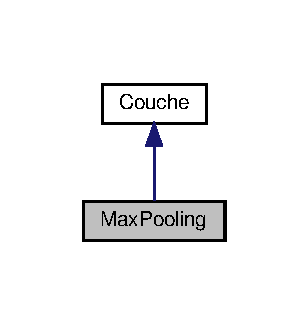
\includegraphics[width=148pt]{class_max_pooling__inherit__graph}
\end{center}
\end{figure}


Graphe de collaboration de Max\+Pooling\+:\nopagebreak
\begin{figure}[H]
\begin{center}
\leavevmode
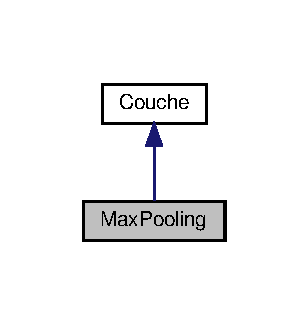
\includegraphics[width=148pt]{class_max_pooling__coll__graph}
\end{center}
\end{figure}
\subsection*{Fonctions membres publiques}
\begin{DoxyCompactItemize}
\item 
\mbox{\Hypertarget{class_max_pooling_aa26ff6fb01b361da3e57dfe77131a20a}\label{class_max_pooling_aa26ff6fb01b361da3e57dfe77131a20a}} 
\hyperlink{class_max_pooling_aa26ff6fb01b361da3e57dfe77131a20a}{Max\+Pooling} (\hyperlink{class_dim_tenseur}{Dim\+Tenseur} din, \hyperlink{class_dim_tenseur}{Dim\+Tenseur} dout, std\+::string no, int pl\+\_\+x, int pl\+\_\+y)
\begin{DoxyCompactList}\small\item\em Constructeur afin d\textquotesingle{}obtenir une image de taille pool\+\_\+x par pool\+\_\+y. \end{DoxyCompactList}\item 
\mbox{\Hypertarget{class_max_pooling_a49e6a67705aacebcc8a58a4d73cd7c58}\label{class_max_pooling_a49e6a67705aacebcc8a58a4d73cd7c58}} 
\hyperlink{class_max_pooling_a49e6a67705aacebcc8a58a4d73cd7c58}{Max\+Pooling} (\hyperlink{class_dim_tenseur}{Dim\+Tenseur} din, \hyperlink{class_dim_tenseur}{Dim\+Tenseur} dout, std\+::string no, int pl)
\begin{DoxyCompactList}\small\item\em Constructeur afin d\textquotesingle{}obtenir une image de taille pool par pool. \end{DoxyCompactList}\item 
\hyperlink{class_tenseur}{Tenseur} \hyperlink{class_max_pooling_a48e0258bf1f949853cfceb2726035fb8}{propagation} (\hyperlink{class_tenseur}{Tenseur} t)
\begin{DoxyCompactList}\small\item\em Méthode permettant la propagation d\textquotesingle{}une couche à une autre. \end{DoxyCompactList}\item 
void \hyperlink{class_max_pooling_ae70dd14b2ebe5963b3a6904ca86857bc}{set\+PoolX} (int pl\+\_\+x)
\begin{DoxyCompactList}\small\item\em Méthode pour fixer le nombre de pixels en dimension x. \end{DoxyCompactList}\item 
void \hyperlink{class_max_pooling_abf21b8f9da67780af60a588a543f7a1b}{set\+PoolY} (int pl\+\_\+y)
\begin{DoxyCompactList}\small\item\em Méthode pour fixer le nombre de pixels en dimension y. \end{DoxyCompactList}\item 
int \hyperlink{class_max_pooling_aa794b6174d54f2be8e6eed4ab09365e9}{get\+PoolX} () const
\begin{DoxyCompactList}\small\item\em Méthode pour obtenir le nombre de pixels fixé pour les images en dimension x. \end{DoxyCompactList}\item 
int \hyperlink{class_max_pooling_a7c72e57c8a90e18804b288f28fde7af0}{get\+PoolY} () const
\begin{DoxyCompactList}\small\item\em Méthode pour obtenir le nombre de pixels fixé pour les images en dimension y. \end{DoxyCompactList}\end{DoxyCompactItemize}


\subsection{Description détaillée}
Classe gérant une couche de \hyperlink{class_max_pooling}{Max\+Pooling}. 

\begin{DoxyAuthor}{Auteur}
Adrien 
\end{DoxyAuthor}
\begin{DoxyVersion}{Version}
1.\+0 
\end{DoxyVersion}
\begin{DoxyDate}{Date}
avril 2019
\end{DoxyDate}
Classe qui va effectuer l\textquotesingle{}opération de redimensionnement des images par la technique du \hyperlink{class_max_pooling}{Max\+Pooling}. 

Définition à la ligne 18 du fichier Max\+Pooling.\+hpp.



\subsection{Documentation des fonctions membres}
\mbox{\Hypertarget{class_max_pooling_aa794b6174d54f2be8e6eed4ab09365e9}\label{class_max_pooling_aa794b6174d54f2be8e6eed4ab09365e9}} 
\index{Max\+Pooling@{Max\+Pooling}!get\+PoolX@{get\+PoolX}}
\index{get\+PoolX@{get\+PoolX}!Max\+Pooling@{Max\+Pooling}}
\subsubsection{\texorpdfstring{get\+Pool\+X()}{getPoolX()}}
{\footnotesize\ttfamily int Max\+Pooling\+::get\+PoolX (\begin{DoxyParamCaption}{ }\end{DoxyParamCaption}) const}



Méthode pour obtenir le nombre de pixels fixé pour les images en dimension x. 

\begin{DoxyReturn}{Renvoie}
Le nombre de pixels en dimension x 
\end{DoxyReturn}


Définition à la ligne 38 du fichier Max\+Pooling.\+cpp.

\mbox{\Hypertarget{class_max_pooling_a7c72e57c8a90e18804b288f28fde7af0}\label{class_max_pooling_a7c72e57c8a90e18804b288f28fde7af0}} 
\index{Max\+Pooling@{Max\+Pooling}!get\+PoolY@{get\+PoolY}}
\index{get\+PoolY@{get\+PoolY}!Max\+Pooling@{Max\+Pooling}}
\subsubsection{\texorpdfstring{get\+Pool\+Y()}{getPoolY()}}
{\footnotesize\ttfamily int Max\+Pooling\+::get\+PoolY (\begin{DoxyParamCaption}{ }\end{DoxyParamCaption}) const}



Méthode pour obtenir le nombre de pixels fixé pour les images en dimension y. 

\begin{DoxyReturn}{Renvoie}
Le nombre de pixels en dimension y 
\end{DoxyReturn}


Définition à la ligne 45 du fichier Max\+Pooling.\+cpp.

\mbox{\Hypertarget{class_max_pooling_a48e0258bf1f949853cfceb2726035fb8}\label{class_max_pooling_a48e0258bf1f949853cfceb2726035fb8}} 
\index{Max\+Pooling@{Max\+Pooling}!propagation@{propagation}}
\index{propagation@{propagation}!Max\+Pooling@{Max\+Pooling}}
\subsubsection{\texorpdfstring{propagation()}{propagation()}}
{\footnotesize\ttfamily \hyperlink{class_tenseur}{Tenseur} Max\+Pooling\+::propagation (\begin{DoxyParamCaption}\item[{\hyperlink{class_tenseur}{Tenseur}}]{t }\end{DoxyParamCaption})\hspace{0.3cm}{\ttfamily [virtual]}}



Méthode permettant la propagation d\textquotesingle{}une couche à une autre. 


\begin{DoxyParams}{Paramètres}
{\em t} & le tenseur \\
\hline
\end{DoxyParams}
\begin{DoxyReturn}{Renvoie}
Le tenseur à l\textquotesingle{}étape d\textquotesingle{}après 
\end{DoxyReturn}


Réimplémentée à partir de \hyperlink{class_couche_a1f0ed59e21020f5d4f37933af4d1b1e5}{Couche}.



Définition à la ligne 17 du fichier Max\+Pooling.\+cpp.

\mbox{\Hypertarget{class_max_pooling_ae70dd14b2ebe5963b3a6904ca86857bc}\label{class_max_pooling_ae70dd14b2ebe5963b3a6904ca86857bc}} 
\index{Max\+Pooling@{Max\+Pooling}!set\+PoolX@{set\+PoolX}}
\index{set\+PoolX@{set\+PoolX}!Max\+Pooling@{Max\+Pooling}}
\subsubsection{\texorpdfstring{set\+Pool\+X()}{setPoolX()}}
{\footnotesize\ttfamily void Max\+Pooling\+::set\+PoolX (\begin{DoxyParamCaption}\item[{int}]{pl\+\_\+x }\end{DoxyParamCaption})}



Méthode pour fixer le nombre de pixels en dimension x. 


\begin{DoxyParams}{Paramètres}
{\em dim\+In} & La dimension du tenseur d\textquotesingle{}entrée \\
\hline
\end{DoxyParams}


Définition à la ligne 24 du fichier Max\+Pooling.\+cpp.

\mbox{\Hypertarget{class_max_pooling_abf21b8f9da67780af60a588a543f7a1b}\label{class_max_pooling_abf21b8f9da67780af60a588a543f7a1b}} 
\index{Max\+Pooling@{Max\+Pooling}!set\+PoolY@{set\+PoolY}}
\index{set\+PoolY@{set\+PoolY}!Max\+Pooling@{Max\+Pooling}}
\subsubsection{\texorpdfstring{set\+Pool\+Y()}{setPoolY()}}
{\footnotesize\ttfamily void Max\+Pooling\+::set\+PoolY (\begin{DoxyParamCaption}\item[{int}]{pl\+\_\+y }\end{DoxyParamCaption})}



Méthode pour fixer le nombre de pixels en dimension y. 


\begin{DoxyParams}{Paramètres}
{\em dim\+In} & La dimension du tenseur de sortie \\
\hline
\end{DoxyParams}


Définition à la ligne 31 du fichier Max\+Pooling.\+cpp.



La documentation de cette classe a été générée à partir des fichiers suivants \+:\begin{DoxyCompactItemize}
\item 
src/deeplearn/archi/Max\+Pooling.\+hpp\item 
src/deeplearn/archi/Max\+Pooling.\+cpp\end{DoxyCompactItemize}

\hypertarget{class_neurone}{}\section{Référence de la classe Neurone}
\label{class_neurone}\index{Neurone@{Neurone}}


Graphe d\textquotesingle{}héritage de Neurone\+:\nopagebreak
\begin{figure}[H]
\begin{center}
\leavevmode
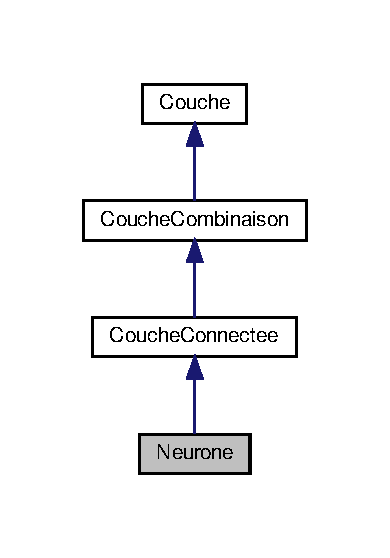
\includegraphics[width=187pt]{class_neurone__inherit__graph}
\end{center}
\end{figure}


Graphe de collaboration de Neurone\+:\nopagebreak
\begin{figure}[H]
\begin{center}
\leavevmode
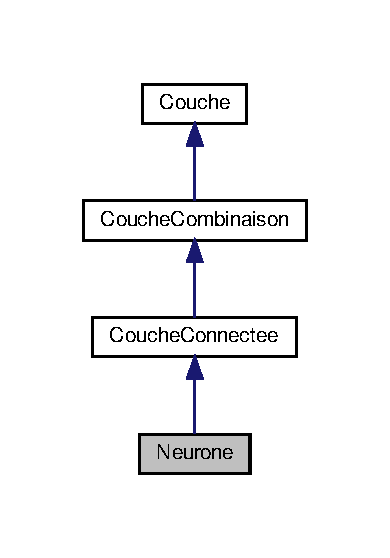
\includegraphics[width=187pt]{class_neurone__coll__graph}
\end{center}
\end{figure}
\subsection*{Fonctions membres publiques}
\begin{DoxyCompactItemize}
\item 
\mbox{\Hypertarget{class_neurone_af50116b497400f2b84f424854971f750}\label{class_neurone_af50116b497400f2b84f424854971f750}} 
\hyperlink{class_neurone_af50116b497400f2b84f424854971f750}{Neurone} (\hyperlink{class_dim_tenseur}{Dim\+Tenseur} din, \hyperlink{class_dim_tenseur}{Dim\+Tenseur} dout, std\+::string no, \hyperlink{class_tenseur}{Tenseur} par)
\begin{DoxyCompactList}\small\item\em Constructeur d\textquotesingle{}un neurone. \end{DoxyCompactList}\end{DoxyCompactItemize}


\subsection{Description détaillée}


Définition à la ligne 17 du fichier Neurone.\+hpp.



La documentation de cette classe a été générée à partir des fichiers suivants \+:\begin{DoxyCompactItemize}
\item 
src/deeplearn/archi/Neurone.\+hpp\item 
src/deeplearn/archi/Neurone.\+cpp\end{DoxyCompactItemize}

\hypertarget{class_optimisateur}{}\section{Référence de la classe Optimisateur}
\label{class_optimisateur}\index{Optimisateur@{Optimisateur}}


Gère l\textquotesingle{}optimisation d\textquotesingle{}un apprentissage.  




{\ttfamily \#include $<$Optimisateur.\+hpp$>$}

\subsection*{Fonctions membres publiques}
\begin{DoxyCompactItemize}
\item 
\mbox{\Hypertarget{class_optimisateur_a6add3f8a05881c495701ced64cb7310e}\label{class_optimisateur_a6add3f8a05881c495701ced64cb7310e}} 
\hyperlink{class_optimisateur_a6add3f8a05881c495701ced64cb7310e}{Optimisateur} (\hyperlink{class_reseau_neurones}{Reseau\+Neurones} reseauN)
\begin{DoxyCompactList}\small\item\em Constructeur d\textquotesingle{}un otpimisateur a partir d\textquotesingle{}un reseau de neurones. \end{DoxyCompactList}\item 
\mbox{\Hypertarget{class_optimisateur_a36f64c4672ec7694a06daad60715bd3a}\label{class_optimisateur_a36f64c4672ec7694a06daad60715bd3a}} 
void \hyperlink{class_optimisateur_a36f64c4672ec7694a06daad60715bd3a}{minimiser} (\hyperlink{class_erreur}{Erreur} err)
\begin{DoxyCompactList}\small\item\em Minimise une erreur donnee. \end{DoxyCompactList}\end{DoxyCompactItemize}


\subsection{Description détaillée}
Gère l\textquotesingle{}optimisation d\textquotesingle{}un apprentissage. 

\begin{DoxyAuthor}{Auteur}
Marion 
\end{DoxyAuthor}
\begin{DoxyVersion}{Version}
1.\+0 
\end{DoxyVersion}
\begin{DoxyDate}{Date}
avril 2019
\end{DoxyDate}
Module permettant le traitement de l\textquotesingle{}optimisation de l\textquotesingle{}erreur lors d\textquotesingle{}un apprentissage. 

Définition à la ligne 19 du fichier Optimisateur.\+hpp.



La documentation de cette classe a été générée à partir du fichier suivant \+:\begin{DoxyCompactItemize}
\item 
src/deeplearn/train/Optimisateur.\+hpp\end{DoxyCompactItemize}

\hypertarget{class_panneau}{}\section{Référence de la classe Panneau}
\label{class_panneau}\index{Panneau@{Panneau}}


Gestion du type \hyperlink{class_panneau}{Panneau}.  




{\ttfamily \#include $<$Panneau.\+hpp$>$}



Graphe d\textquotesingle{}héritage de Panneau\+:\nopagebreak
\begin{figure}[H]
\begin{center}
\leavevmode
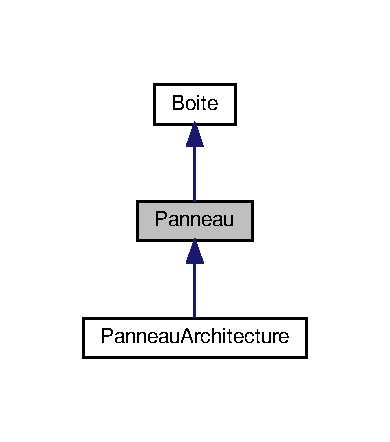
\includegraphics[width=187pt]{class_panneau__inherit__graph}
\end{center}
\end{figure}


Graphe de collaboration de Panneau\+:\nopagebreak
\begin{figure}[H]
\begin{center}
\leavevmode
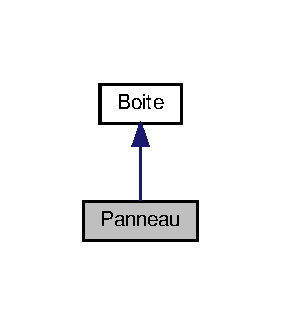
\includegraphics[width=135pt]{class_panneau__coll__graph}
\end{center}
\end{figure}
\subsection*{Fonctions membres publiques}
\begin{DoxyCompactItemize}
\item 
\mbox{\Hypertarget{class_panneau_a8fb82bab20bdc45acfe9234f3fb9a38e}\label{class_panneau_a8fb82bab20bdc45acfe9234f3fb9a38e}} 
\hyperlink{class_panneau_a8fb82bab20bdc45acfe9234f3fb9a38e}{Boite\+Architecture} ()
\begin{DoxyCompactList}\small\item\em Constructeur d\textquotesingle{}une boite d\textquotesingle{}architecture. \end{DoxyCompactList}\item 
\hyperlink{class_panneau_a2c86ba058850b199a83eb4a35541531c}{Boite\+Architecture} (\hyperlink{class_reseau_neurones}{Reseau\+Neurones} rn)
\begin{DoxyCompactList}\small\item\em Constucteur prenant en paramètre un reseau de neurones. \end{DoxyCompactList}\item 
void \hyperlink{class_panneau_a0990ee55f48bc73a20f9079fa8e2582d}{afficher} (\hyperlink{class_reseau_neurones}{Reseau\+Neurones} rn)
\begin{DoxyCompactList}\small\item\em Méthode permettant l\textquotesingle{}affichage d\textquotesingle{}un reseau de neurones. \end{DoxyCompactList}\item 
\mbox{\Hypertarget{class_panneau_a6d15af2ca1be32f371599285f3edbbcc}\label{class_panneau_a6d15af2ca1be32f371599285f3edbbcc}} 
\hyperlink{class_panneau_a6d15af2ca1be32f371599285f3edbbcc}{Panneau} ()
\begin{DoxyCompactList}\small\item\em Constructeur du panneau vide. \end{DoxyCompactList}\item 
\mbox{\Hypertarget{class_panneau_a390b3758b0280bfa67add85464775016}\label{class_panneau_a390b3758b0280bfa67add85464775016}} 
void \hyperlink{class_panneau_a390b3758b0280bfa67add85464775016}{sauvegarder\+RN} ()
\begin{DoxyCompactList}\small\item\em Méthode permettant la sauvegarde d\textquotesingle{}un Reseau de Neurones. \end{DoxyCompactList}\item 
\mbox{\Hypertarget{class_panneau_a3f7414f7c42e6378fbea049c246db2a9}\label{class_panneau_a3f7414f7c42e6378fbea049c246db2a9}} 
void {\bfseries sauvegarder\+RN} (string nom\+Fichier)
\item 
\hyperlink{class_reseau_neurones}{Reseau\+Neurones} \hyperlink{class_panneau_a8ed7e5db0c0c8a0da729d3c785032643}{get\+Reseau\+Neurones} ()
\begin{DoxyCompactList}\small\item\em getteur permettant d\textquotesingle{}acceder au Reseau de Neurones en attribut de la classe \end{DoxyCompactList}\end{DoxyCompactItemize}


\subsection{Description détaillée}
Gestion du type \hyperlink{class_panneau}{Panneau}. 

\begin{DoxyAuthor}{Auteur}
Samra 
\end{DoxyAuthor}
\begin{DoxyVersion}{Version}
1.\+0 
\end{DoxyVersion}
\begin{DoxyDate}{Date}
avril 2019 
\end{DoxyDate}


Définition à la ligne 20 du fichier Boite\+Architecture.\+hpp.



\subsection{Documentation des fonctions membres}
\mbox{\Hypertarget{class_panneau_a0990ee55f48bc73a20f9079fa8e2582d}\label{class_panneau_a0990ee55f48bc73a20f9079fa8e2582d}} 
\index{Panneau@{Panneau}!afficher@{afficher}}
\index{afficher@{afficher}!Panneau@{Panneau}}
\subsubsection{\texorpdfstring{afficher()}{afficher()}}
{\footnotesize\ttfamily void Panneau\+::afficher (\begin{DoxyParamCaption}\item[{\hyperlink{class_reseau_neurones}{Reseau\+Neurones}}]{rn }\end{DoxyParamCaption})}



Méthode permettant l\textquotesingle{}affichage d\textquotesingle{}un reseau de neurones. 


\begin{DoxyParams}{Paramètres}
{\em rn} & le réseau de neurones \\
\hline
\end{DoxyParams}
\mbox{\Hypertarget{class_panneau_a2c86ba058850b199a83eb4a35541531c}\label{class_panneau_a2c86ba058850b199a83eb4a35541531c}} 
\index{Panneau@{Panneau}!Boite\+Architecture@{Boite\+Architecture}}
\index{Boite\+Architecture@{Boite\+Architecture}!Panneau@{Panneau}}
\subsubsection{\texorpdfstring{Boite\+Architecture()}{BoiteArchitecture()}}
{\footnotesize\ttfamily Panneau\+::\+Boite\+Architecture (\begin{DoxyParamCaption}\item[{\hyperlink{class_reseau_neurones}{Reseau\+Neurones}}]{rn }\end{DoxyParamCaption})}



Constucteur prenant en paramètre un reseau de neurones. 


\begin{DoxyParams}{Paramètres}
{\em rn} & un réseau de neurones préalablement défini \\
\hline
\end{DoxyParams}
\mbox{\Hypertarget{class_panneau_a8ed7e5db0c0c8a0da729d3c785032643}\label{class_panneau_a8ed7e5db0c0c8a0da729d3c785032643}} 
\index{Panneau@{Panneau}!get\+Reseau\+Neurones@{get\+Reseau\+Neurones}}
\index{get\+Reseau\+Neurones@{get\+Reseau\+Neurones}!Panneau@{Panneau}}
\subsubsection{\texorpdfstring{get\+Reseau\+Neurones()}{getReseauNeurones()}}
{\footnotesize\ttfamily \hyperlink{class_reseau_neurones}{Reseau\+Neurones} Panneau\+::get\+Reseau\+Neurones (\begin{DoxyParamCaption}{ }\end{DoxyParamCaption})}



getteur permettant d\textquotesingle{}acceder au Reseau de Neurones en attribut de la classe 

\begin{DoxyReturn}{Renvoie}
le Reseau de neurones en attribut de la classe \hyperlink{class_panneau}{Panneau} 
\end{DoxyReturn}


La documentation de cette classe a été générée à partir des fichiers suivants \+:\begin{DoxyCompactItemize}
\item 
src/ihm/Boite\+Architecture.\+hpp\item 
src/ihm/Panneau.\+hpp\end{DoxyCompactItemize}

\hypertarget{class_panneau_architecture}{}\section{Référence de la classe Panneau\+Architecture}
\label{class_panneau_architecture}\index{Panneau\+Architecture@{Panneau\+Architecture}}


???  




{\ttfamily \#include $<$Panneau\+Architecture.\+hpp$>$}



Graphe d\textquotesingle{}héritage de Panneau\+Architecture\+:\nopagebreak
\begin{figure}[H]
\begin{center}
\leavevmode
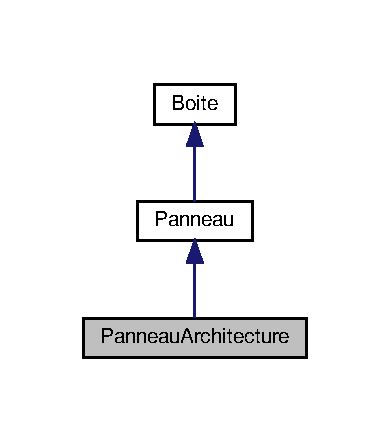
\includegraphics[width=187pt]{class_panneau_architecture__inherit__graph}
\end{center}
\end{figure}


Graphe de collaboration de Panneau\+Architecture\+:\nopagebreak
\begin{figure}[H]
\begin{center}
\leavevmode
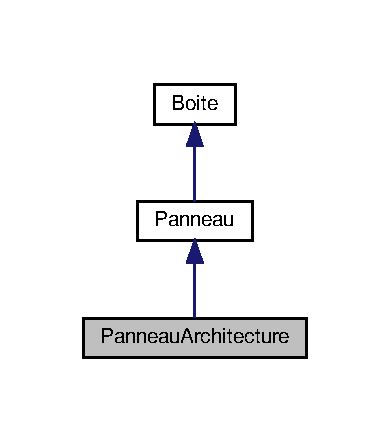
\includegraphics[width=187pt]{class_panneau_architecture__coll__graph}
\end{center}
\end{figure}
\subsection*{Fonctions membres publiques}
\begin{DoxyCompactItemize}
\item 
\mbox{\Hypertarget{class_panneau_architecture_a1143575686655c5088510a94eac5c787}\label{class_panneau_architecture_a1143575686655c5088510a94eac5c787}} 
\hyperlink{class_panneau_architecture_a1143575686655c5088510a94eac5c787}{Panneau\+Architecture} ()
\begin{DoxyCompactList}\small\item\em Constructeur du panneau vide. \end{DoxyCompactList}\item 
\mbox{\Hypertarget{class_panneau_architecture_affc6f75cb58e1c50aad26510bc2c25ea}\label{class_panneau_architecture_affc6f75cb58e1c50aad26510bc2c25ea}} 
void \hyperlink{class_panneau_architecture_affc6f75cb58e1c50aad26510bc2c25ea}{ajouter\+Couche} ()
\begin{DoxyCompactList}\small\item\em Méthode permettant l\textquotesingle{}ajout d\textquotesingle{}une couche. \end{DoxyCompactList}\item 
\mbox{\Hypertarget{class_panneau_architecture_a49eb9dea42db4fb1b16d91cfc1c789c3}\label{class_panneau_architecture_a49eb9dea42db4fb1b16d91cfc1c789c3}} 
void \hyperlink{class_panneau_architecture_a49eb9dea42db4fb1b16d91cfc1c789c3}{ajouter\+RN} ()
\begin{DoxyCompactList}\small\item\em Méthode permettant l\textquotesingle{}ajout d\textquotesingle{}un Reseau de Neurones. \end{DoxyCompactList}\item 
\mbox{\Hypertarget{class_panneau_architecture_ac623d04cebc723d2e590712a337cd5ab}\label{class_panneau_architecture_ac623d04cebc723d2e590712a337cd5ab}} 
void \hyperlink{class_panneau_architecture_ac623d04cebc723d2e590712a337cd5ab}{ajouter\+Liaison} ()
\begin{DoxyCompactList}\small\item\em Méthode permettant d\textquotesingle{}ajouter une liaison. \end{DoxyCompactList}\item 
\mbox{\Hypertarget{class_panneau_architecture_a4b90aec081c2b2d0b2a3c3207183bd3f}\label{class_panneau_architecture_a4b90aec081c2b2d0b2a3c3207183bd3f}} 
void \hyperlink{class_panneau_architecture_a4b90aec081c2b2d0b2a3c3207183bd3f}{supprimer\+Couche} ()
\begin{DoxyCompactList}\small\item\em Méthode permettant la suppression d\textquotesingle{}une couche. \end{DoxyCompactList}\item 
\mbox{\Hypertarget{class_panneau_architecture_af6e7d198ef558f75d8826cf9d52a1248}\label{class_panneau_architecture_af6e7d198ef558f75d8826cf9d52a1248}} 
void \hyperlink{class_panneau_architecture_af6e7d198ef558f75d8826cf9d52a1248}{supprimer\+Liaison} ()
\begin{DoxyCompactList}\small\item\em Méthode permettant de supprimer une liaison. \end{DoxyCompactList}\item 
\mbox{\Hypertarget{class_panneau_architecture_a7670673acd7e9eb1e77e2cb5eb929079}\label{class_panneau_architecture_a7670673acd7e9eb1e77e2cb5eb929079}} 
void \hyperlink{class_panneau_architecture_a7670673acd7e9eb1e77e2cb5eb929079}{select\+Couche} (\hyperlink{class_couche}{Couche})
\begin{DoxyCompactList}\small\item\em Méthode mettant à jour la ccouche selectionnée. \end{DoxyCompactList}\item 
\mbox{\Hypertarget{class_panneau_architecture_a2e4ab85ad5fbc8801bf7ea3fab0ea197}\label{class_panneau_architecture_a2e4ab85ad5fbc8801bf7ea3fab0ea197}} 
void \hyperlink{class_panneau_architecture_a2e4ab85ad5fbc8801bf7ea3fab0ea197}{select\+Liaison} (\hyperlink{class_couche}{Couche}, \hyperlink{class_couche}{Couche})
\begin{DoxyCompactList}\small\item\em Méthode mettant à jour la liaison selectionnée. \end{DoxyCompactList}\item 
\mbox{\Hypertarget{class_panneau_architecture_a77c5b0be02105db0a55ec022cc319e4b}\label{class_panneau_architecture_a77c5b0be02105db0a55ec022cc319e4b}} 
\hyperlink{class_couche}{Couche} \hyperlink{class_panneau_architecture_a77c5b0be02105db0a55ec022cc319e4b}{get\+Couche\+Selectionnee} ()
\begin{DoxyCompactList}\small\item\em Méthode permettant d\textquotesingle{}acceder a la couche selectionnée. \end{DoxyCompactList}\item 
\mbox{\Hypertarget{class_panneau_architecture_a8502f49ce3c223fa9cfe73b6621d5da8}\label{class_panneau_architecture_a8502f49ce3c223fa9cfe73b6621d5da8}} 
pair$<$ \hyperlink{class_couche}{Couche}, \hyperlink{class_couche}{Couche} $>$ \hyperlink{class_panneau_architecture_a8502f49ce3c223fa9cfe73b6621d5da8}{get\+Liaison} ()
\begin{DoxyCompactList}\small\item\em Méthode permettant d\textquotesingle{}acceder à la liaisonn selectionnée. \end{DoxyCompactList}\end{DoxyCompactItemize}


\subsection{Description détaillée}
??? 

\begin{DoxyAuthor}{Auteur}
??? 
\end{DoxyAuthor}
\begin{DoxyVersion}{Version}
1.\+0 
\end{DoxyVersion}
\begin{DoxyDate}{Date}
avril 2019
\end{DoxyDate}
Regroupe les differentes boites ( choix couche, RN ,connexion ) dans un même \hyperlink{class_panneau}{Panneau} 

Définition à la ligne 22 du fichier Panneau\+Architecture.\+hpp.



La documentation de cette classe a été générée à partir du fichier suivant \+:\begin{DoxyCompactItemize}
\item 
src/ihm/Panneau\+Architecture.\+hpp\end{DoxyCompactItemize}

\hypertarget{class_parametres_apprentissage}{}\section{Référence de la classe Parametres\+Apprentissage}
\label{class_parametres_apprentissage}\index{Parametres\+Apprentissage@{Parametres\+Apprentissage}}


Gère les parametres d\textquotesingle{}apprentissage du réseau de neurones.  




{\ttfamily \#include $<$Parametres\+Apprentissage.\+hpp$>$}

\subsection*{Fonctions membres publiques}
\begin{DoxyCompactItemize}
\item 
\mbox{\Hypertarget{class_parametres_apprentissage_a0912bbe1ac8b0f2e0248edf049ef0b53}\label{class_parametres_apprentissage_a0912bbe1ac8b0f2e0248edf049ef0b53}} 
\hyperlink{class_parametres_apprentissage_a0912bbe1ac8b0f2e0248edf049ef0b53}{Parametres\+Apprentissage} ()
\begin{DoxyCompactList}\small\item\em Constructeur des parametres d\textquotesingle{}apprentissage. \end{DoxyCompactList}\item 
int \hyperlink{class_parametres_apprentissage_ad4342b1543901201ad28b1da5c11dc26}{get\+Nb\+Epoques} ()
\begin{DoxyCompactList}\small\item\em Retourne le nombre d\textquotesingle{}epoques de l\textquotesingle{}apprentissage. \end{DoxyCompactList}\item 
double \hyperlink{class_parametres_apprentissage_aa5b6d225498ee1270996ace135745fdd}{get\+Taux\+Apprentissage} ()
\begin{DoxyCompactList}\small\item\em Retourne le taux d\textquotesingle{}apprentissage du reseau. \end{DoxyCompactList}\item 
void \hyperlink{class_parametres_apprentissage_a0b424fc552461e9e13d51024bd071470}{set\+Nb\+Epoques} (int ep)
\begin{DoxyCompactList}\small\item\em Met a jour le nombre d\textquotesingle{}epoques de l\textquotesingle{}apprentissage. \end{DoxyCompactList}\item 
void \hyperlink{class_parametres_apprentissage_a13b6b90a24b4733c6b465aa74a1abda9}{set\+Taux\+Apprentissage} (double ta)
\begin{DoxyCompactList}\small\item\em Met a jour le taux d\textquotesingle{}apprentissage du reseau. \end{DoxyCompactList}\end{DoxyCompactItemize}


\subsection{Description détaillée}
Gère les parametres d\textquotesingle{}apprentissage du réseau de neurones. 

\begin{DoxyAuthor}{Auteur}
Marion 
\end{DoxyAuthor}
\begin{DoxyVersion}{Version}
1.\+0 
\end{DoxyVersion}
\begin{DoxyDate}{Date}
avril 2019
\end{DoxyDate}
Module permettant le choix des parametres de l\textquotesingle{}apprentissage. Il permet également leur récupération. 

Définition à la ligne 16 du fichier Parametres\+Apprentissage.\+hpp.



\subsection{Documentation des fonctions membres}
\mbox{\Hypertarget{class_parametres_apprentissage_ad4342b1543901201ad28b1da5c11dc26}\label{class_parametres_apprentissage_ad4342b1543901201ad28b1da5c11dc26}} 
\index{Parametres\+Apprentissage@{Parametres\+Apprentissage}!get\+Nb\+Epoques@{get\+Nb\+Epoques}}
\index{get\+Nb\+Epoques@{get\+Nb\+Epoques}!Parametres\+Apprentissage@{Parametres\+Apprentissage}}
\subsubsection{\texorpdfstring{get\+Nb\+Epoques()}{getNbEpoques()}}
{\footnotesize\ttfamily int Parametres\+Apprentissage\+::get\+Nb\+Epoques (\begin{DoxyParamCaption}{ }\end{DoxyParamCaption})}



Retourne le nombre d\textquotesingle{}epoques de l\textquotesingle{}apprentissage. 

\begin{DoxyReturn}{Renvoie}
le nombre d\textquotesingle{}epoques 
\end{DoxyReturn}
\mbox{\Hypertarget{class_parametres_apprentissage_aa5b6d225498ee1270996ace135745fdd}\label{class_parametres_apprentissage_aa5b6d225498ee1270996ace135745fdd}} 
\index{Parametres\+Apprentissage@{Parametres\+Apprentissage}!get\+Taux\+Apprentissage@{get\+Taux\+Apprentissage}}
\index{get\+Taux\+Apprentissage@{get\+Taux\+Apprentissage}!Parametres\+Apprentissage@{Parametres\+Apprentissage}}
\subsubsection{\texorpdfstring{get\+Taux\+Apprentissage()}{getTauxApprentissage()}}
{\footnotesize\ttfamily double Parametres\+Apprentissage\+::get\+Taux\+Apprentissage (\begin{DoxyParamCaption}{ }\end{DoxyParamCaption})}



Retourne le taux d\textquotesingle{}apprentissage du reseau. 

\begin{DoxyReturn}{Renvoie}
le tauc d\textquotesingle{}apprentissage $\ast$ 
\end{DoxyReturn}
\mbox{\Hypertarget{class_parametres_apprentissage_a0b424fc552461e9e13d51024bd071470}\label{class_parametres_apprentissage_a0b424fc552461e9e13d51024bd071470}} 
\index{Parametres\+Apprentissage@{Parametres\+Apprentissage}!set\+Nb\+Epoques@{set\+Nb\+Epoques}}
\index{set\+Nb\+Epoques@{set\+Nb\+Epoques}!Parametres\+Apprentissage@{Parametres\+Apprentissage}}
\subsubsection{\texorpdfstring{set\+Nb\+Epoques()}{setNbEpoques()}}
{\footnotesize\ttfamily void Parametres\+Apprentissage\+::set\+Nb\+Epoques (\begin{DoxyParamCaption}\item[{int}]{ep }\end{DoxyParamCaption})}



Met a jour le nombre d\textquotesingle{}epoques de l\textquotesingle{}apprentissage. 


\begin{DoxyParams}{Paramètres}
{\em ep} & le nombre d\textquotesingle{}epoques de l\textquotesingle{}apprentissage \\
\hline
\end{DoxyParams}
\mbox{\Hypertarget{class_parametres_apprentissage_a13b6b90a24b4733c6b465aa74a1abda9}\label{class_parametres_apprentissage_a13b6b90a24b4733c6b465aa74a1abda9}} 
\index{Parametres\+Apprentissage@{Parametres\+Apprentissage}!set\+Taux\+Apprentissage@{set\+Taux\+Apprentissage}}
\index{set\+Taux\+Apprentissage@{set\+Taux\+Apprentissage}!Parametres\+Apprentissage@{Parametres\+Apprentissage}}
\subsubsection{\texorpdfstring{set\+Taux\+Apprentissage()}{setTauxApprentissage()}}
{\footnotesize\ttfamily void Parametres\+Apprentissage\+::set\+Taux\+Apprentissage (\begin{DoxyParamCaption}\item[{double}]{ta }\end{DoxyParamCaption})}



Met a jour le taux d\textquotesingle{}apprentissage du reseau. 


\begin{DoxyParams}{Paramètres}
{\em ta} & le taux d\textquotesingle{}apprentissage \\
\hline
\end{DoxyParams}


La documentation de cette classe a été générée à partir du fichier suivant \+:\begin{DoxyCompactItemize}
\item 
src/deeplearn/train/Parametres\+Apprentissage.\+hpp\end{DoxyCompactItemize}

\hypertarget{class_pretraitement}{}\section{Référence de la classe Pretraitement}
\label{class_pretraitement}\index{Pretraitement@{Pretraitement}}


Gère le pretraitement des donnees necessaires a l\textquotesingle{}apprentissage.  




{\ttfamily \#include $<$Pretraitement.\+hpp$>$}

\subsection*{Fonctions membres publiques statiques}
\begin{DoxyCompactItemize}
\item 
static \hyperlink{class_donnees}{Donnees} \hyperlink{class_pretraitement_a5f53fc5ecf4893d40577aceb269e97b5}{charger\+Donnees} (std\+::string nom\+Dossier)
\begin{DoxyCompactList}\small\item\em Charge les donnees du dossier. \end{DoxyCompactList}\item 
static \hyperlink{class_reseau_neurones}{Reseau\+Neurones} \hyperlink{class_pretraitement_a2d1e9cdbe1b865565f63c435923ec8e3}{charger\+RN} (std\+::string nom\+Fichier)
\begin{DoxyCompactList}\small\item\em Charge le reseau de neurones contenu dans un fichier. \end{DoxyCompactList}\item 
static \hyperlink{class_tenseur}{Tenseur} \hyperlink{class_pretraitement_a98c809577fe15166c5a9be25daff64a1}{image\+To\+Tenseur} (std\+::string nom\+Fichier)
\begin{DoxyCompactList}\small\item\em Transforme l\textquotesingle{}image d\textquotesingle{}entree en un tenseur. \end{DoxyCompactList}\item 
static \hyperlink{class_tenseur}{Tenseur} \hyperlink{class_pretraitement_a588810b1b86e11464cea64443358ae5a}{csv\+To\+Tenseur} (std\+::string nom\+Fichier)
\begin{DoxyCompactList}\small\item\em Transforme un fichier csv en tenseur. \end{DoxyCompactList}\item 
static void \hyperlink{class_pretraitement_a3d7be2ef2f1c6b0b8e3f1898110740bc}{normaliser} (\hyperlink{class_tenseur}{Tenseur} \&t, double min\+Norm, double max\+Norm, double min\+Valeur, double max\+Valeur)
\begin{DoxyCompactList}\small\item\em Normalise le tenseur passe en entree en fonction des autres parametres. \end{DoxyCompactList}\item 
static void \hyperlink{class_pretraitement_a68c5f7dc52d76fe0ff1f2794c4de40d7}{denormaliser} (\hyperlink{class_tenseur}{Tenseur} \&t, double min\+Norm, double max\+Norm, double min\+Valeur, double max\+Valeur)
\begin{DoxyCompactList}\small\item\em Denormalise le tenseur passe en entree en fonction des autres parametres. \end{DoxyCompactList}\end{DoxyCompactItemize}


\subsection{Description détaillée}
Gère le pretraitement des donnees necessaires a l\textquotesingle{}apprentissage. 

\begin{DoxyAuthor}{Auteur}
Marion 
\end{DoxyAuthor}
\begin{DoxyVersion}{Version}
1.\+0 
\end{DoxyVersion}
\begin{DoxyDate}{Date}
avril 2019
\end{DoxyDate}
Module permettant le pretraitement des donnees necessaires avant l\textquotesingle{}apprentissage. 

Définition à la ligne 18 du fichier Pretraitement.\+hpp.



\subsection{Documentation des fonctions membres}
\mbox{\Hypertarget{class_pretraitement_a5f53fc5ecf4893d40577aceb269e97b5}\label{class_pretraitement_a5f53fc5ecf4893d40577aceb269e97b5}} 
\index{Pretraitement@{Pretraitement}!charger\+Donnees@{charger\+Donnees}}
\index{charger\+Donnees@{charger\+Donnees}!Pretraitement@{Pretraitement}}
\subsubsection{\texorpdfstring{charger\+Donnees()}{chargerDonnees()}}
{\footnotesize\ttfamily static \hyperlink{class_donnees}{Donnees} Pretraitement\+::charger\+Donnees (\begin{DoxyParamCaption}\item[{std\+::string}]{nom\+Dossier }\end{DoxyParamCaption})\hspace{0.3cm}{\ttfamily [static]}}



Charge les donnees du dossier. 


\begin{DoxyParams}{Paramètres}
{\em nom\+Dossier} & le nom du dossier dans lequel se trouve les donnees a recuperer \\
\hline
\end{DoxyParams}
\mbox{\Hypertarget{class_pretraitement_a2d1e9cdbe1b865565f63c435923ec8e3}\label{class_pretraitement_a2d1e9cdbe1b865565f63c435923ec8e3}} 
\index{Pretraitement@{Pretraitement}!charger\+RN@{charger\+RN}}
\index{charger\+RN@{charger\+RN}!Pretraitement@{Pretraitement}}
\subsubsection{\texorpdfstring{charger\+R\+N()}{chargerRN()}}
{\footnotesize\ttfamily static \hyperlink{class_reseau_neurones}{Reseau\+Neurones} Pretraitement\+::charger\+RN (\begin{DoxyParamCaption}\item[{std\+::string}]{nom\+Fichier }\end{DoxyParamCaption})\hspace{0.3cm}{\ttfamily [static]}}



Charge le reseau de neurones contenu dans un fichier. 


\begin{DoxyParams}{Paramètres}
{\em nom\+Fichier} & le nom du fichier dans lequel se trouve le reseau de neurones a recuperer \\
\hline
\end{DoxyParams}
\mbox{\Hypertarget{class_pretraitement_a588810b1b86e11464cea64443358ae5a}\label{class_pretraitement_a588810b1b86e11464cea64443358ae5a}} 
\index{Pretraitement@{Pretraitement}!csv\+To\+Tenseur@{csv\+To\+Tenseur}}
\index{csv\+To\+Tenseur@{csv\+To\+Tenseur}!Pretraitement@{Pretraitement}}
\subsubsection{\texorpdfstring{csv\+To\+Tenseur()}{csvToTenseur()}}
{\footnotesize\ttfamily static \hyperlink{class_tenseur}{Tenseur} Pretraitement\+::csv\+To\+Tenseur (\begin{DoxyParamCaption}\item[{std\+::string}]{nom\+Fichier }\end{DoxyParamCaption})\hspace{0.3cm}{\ttfamily [static]}}



Transforme un fichier csv en tenseur. 


\begin{DoxyParams}{Paramètres}
{\em nom\+Fichier} & le nom du fichier csv a transformer en tenseur \\
\hline
\end{DoxyParams}
\mbox{\Hypertarget{class_pretraitement_a68c5f7dc52d76fe0ff1f2794c4de40d7}\label{class_pretraitement_a68c5f7dc52d76fe0ff1f2794c4de40d7}} 
\index{Pretraitement@{Pretraitement}!denormaliser@{denormaliser}}
\index{denormaliser@{denormaliser}!Pretraitement@{Pretraitement}}
\subsubsection{\texorpdfstring{denormaliser()}{denormaliser()}}
{\footnotesize\ttfamily static void Pretraitement\+::denormaliser (\begin{DoxyParamCaption}\item[{\hyperlink{class_tenseur}{Tenseur} \&}]{t,  }\item[{double}]{min\+Norm,  }\item[{double}]{max\+Norm,  }\item[{double}]{min\+Valeur,  }\item[{double}]{max\+Valeur }\end{DoxyParamCaption})\hspace{0.3cm}{\ttfamily [static]}}



Denormalise le tenseur passe en entree en fonction des autres parametres. 


\begin{DoxyParams}{Paramètres}
{\em t} & le tenseur a normalise \\
\hline
{\em min\+Norm} & la norme minimale \\
\hline
{\em max\+Norm} & la norme maximale \\
\hline
{\em min\+Valeur} & la valeur minimale \\
\hline
{\em max\+Valeur} & la valeur maximale \\
\hline
\end{DoxyParams}
\mbox{\Hypertarget{class_pretraitement_a98c809577fe15166c5a9be25daff64a1}\label{class_pretraitement_a98c809577fe15166c5a9be25daff64a1}} 
\index{Pretraitement@{Pretraitement}!image\+To\+Tenseur@{image\+To\+Tenseur}}
\index{image\+To\+Tenseur@{image\+To\+Tenseur}!Pretraitement@{Pretraitement}}
\subsubsection{\texorpdfstring{image\+To\+Tenseur()}{imageToTenseur()}}
{\footnotesize\ttfamily static \hyperlink{class_tenseur}{Tenseur} Pretraitement\+::image\+To\+Tenseur (\begin{DoxyParamCaption}\item[{std\+::string}]{nom\+Fichier }\end{DoxyParamCaption})\hspace{0.3cm}{\ttfamily [static]}}



Transforme l\textquotesingle{}image d\textquotesingle{}entree en un tenseur. 


\begin{DoxyParams}{Paramètres}
{\em nom\+Fichier} & le nom du fichier image a transformer en tenseur \\
\hline
\end{DoxyParams}
\mbox{\Hypertarget{class_pretraitement_a3d7be2ef2f1c6b0b8e3f1898110740bc}\label{class_pretraitement_a3d7be2ef2f1c6b0b8e3f1898110740bc}} 
\index{Pretraitement@{Pretraitement}!normaliser@{normaliser}}
\index{normaliser@{normaliser}!Pretraitement@{Pretraitement}}
\subsubsection{\texorpdfstring{normaliser()}{normaliser()}}
{\footnotesize\ttfamily static void Pretraitement\+::normaliser (\begin{DoxyParamCaption}\item[{\hyperlink{class_tenseur}{Tenseur} \&}]{t,  }\item[{double}]{min\+Norm,  }\item[{double}]{max\+Norm,  }\item[{double}]{min\+Valeur,  }\item[{double}]{max\+Valeur }\end{DoxyParamCaption})\hspace{0.3cm}{\ttfamily [static]}}



Normalise le tenseur passe en entree en fonction des autres parametres. 


\begin{DoxyParams}{Paramètres}
{\em t} & le tenseur a normalise \\
\hline
{\em min\+Norm} & la norme minimale \\
\hline
{\em max\+Norm} & la norme maximale \\
\hline
{\em min\+Valeur} & la valeur minimale \\
\hline
{\em max\+Valeur} & la valeur maximale \\
\hline
\end{DoxyParams}


La documentation de cette classe a été générée à partir du fichier suivant \+:\begin{DoxyCompactItemize}
\item 
src/pretraitement/Pretraitement.\+hpp\end{DoxyCompactItemize}

\hypertarget{class_re_l_u}{}\section{Référence de la classe Re\+LU}
\label{class_re_l_u}\index{Re\+LU@{Re\+LU}}


Graphe d\textquotesingle{}héritage de Re\+LU\+:\nopagebreak
\begin{figure}[H]
\begin{center}
\leavevmode
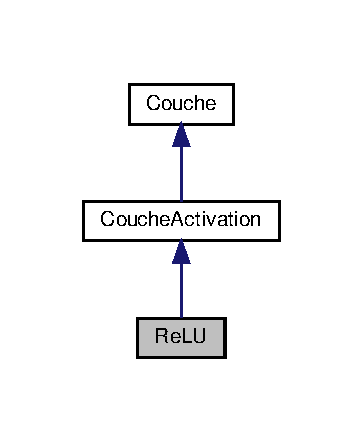
\includegraphics[width=174pt]{class_re_l_u__inherit__graph}
\end{center}
\end{figure}


Graphe de collaboration de Re\+LU\+:\nopagebreak
\begin{figure}[H]
\begin{center}
\leavevmode
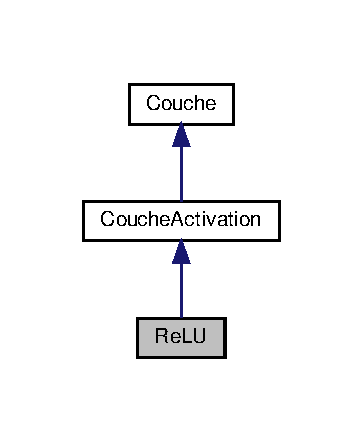
\includegraphics[width=174pt]{class_re_l_u__coll__graph}
\end{center}
\end{figure}
\subsection*{Fonctions membres publiques}
\begin{DoxyCompactItemize}
\item 
\mbox{\Hypertarget{class_re_l_u_a818c59b2b84777493cdfb399d896559c}\label{class_re_l_u_a818c59b2b84777493cdfb399d896559c}} 
\hyperlink{class_re_l_u_a818c59b2b84777493cdfb399d896559c}{Re\+LU} (\hyperlink{class_dim_tenseur}{Dim\+Tenseur} din, \hyperlink{class_dim_tenseur}{Dim\+Tenseur} dout, std\+::string no)
\begin{DoxyCompactList}\small\item\em Constructeur de la fonction \hyperlink{class_re_l_u}{Re\+LU}. \end{DoxyCompactList}\item 
\hyperlink{class_tenseur}{Tenseur} \hyperlink{class_re_l_u_a0d42917d6a9124571b0b467c81bce38a}{propagation} (\hyperlink{class_tenseur}{Tenseur} t)
\begin{DoxyCompactList}\small\item\em Méthode permettant la propagation d\textquotesingle{}une couche à une autre. \end{DoxyCompactList}\end{DoxyCompactItemize}


\subsection{Description détaillée}


Définition à la ligne 17 du fichier Re\+L\+U.\+hpp.



\subsection{Documentation des fonctions membres}
\mbox{\Hypertarget{class_re_l_u_a0d42917d6a9124571b0b467c81bce38a}\label{class_re_l_u_a0d42917d6a9124571b0b467c81bce38a}} 
\index{Re\+LU@{Re\+LU}!propagation@{propagation}}
\index{propagation@{propagation}!Re\+LU@{Re\+LU}}
\subsubsection{\texorpdfstring{propagation()}{propagation()}}
{\footnotesize\ttfamily \hyperlink{class_tenseur}{Tenseur} Re\+L\+U\+::propagation (\begin{DoxyParamCaption}\item[{\hyperlink{class_tenseur}{Tenseur}}]{t }\end{DoxyParamCaption})\hspace{0.3cm}{\ttfamily [virtual]}}



Méthode permettant la propagation d\textquotesingle{}une couche à une autre. 


\begin{DoxyParams}{Paramètres}
{\em t} & le tenseur d\textquotesingle{}entree \\
\hline
\end{DoxyParams}
\begin{DoxyReturn}{Renvoie}
la sortie de la fonction \hyperlink{class_re_l_u}{Re\+LU} 
\end{DoxyReturn}


Réimplémentée à partir de \hyperlink{class_couche_a1f0ed59e21020f5d4f37933af4d1b1e5}{Couche}.



Définition à la ligne 8 du fichier Re\+Lu.\+cpp.



La documentation de cette classe a été générée à partir des fichiers suivants \+:\begin{DoxyCompactItemize}
\item 
src/deeplearn/archi/Re\+L\+U.\+hpp\item 
src/deeplearn/archi/Re\+Lu.\+cpp\end{DoxyCompactItemize}

\hypertarget{class_reseau_neurones}{}\section{Référence de la classe Reseau\+Neurones}
\label{class_reseau_neurones}\index{Reseau\+Neurones@{Reseau\+Neurones}}


Classe liée à la création du réseau de neurones.  




{\ttfamily \#include $<$Reseau\+Neurones.\+hpp$>$}



Graphe d\textquotesingle{}héritage de Reseau\+Neurones\+:\nopagebreak
\begin{figure}[H]
\begin{center}
\leavevmode
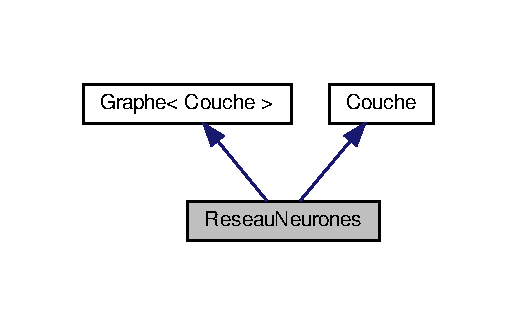
\includegraphics[width=248pt]{class_reseau_neurones__inherit__graph}
\end{center}
\end{figure}


Graphe de collaboration de Reseau\+Neurones\+:\nopagebreak
\begin{figure}[H]
\begin{center}
\leavevmode
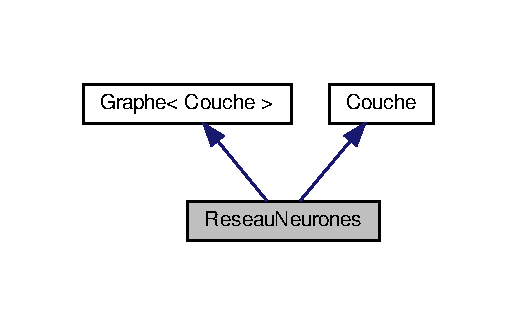
\includegraphics[width=248pt]{class_reseau_neurones__coll__graph}
\end{center}
\end{figure}
\subsection*{Fonctions membres publiques}
\begin{DoxyCompactItemize}
\item 
\mbox{\Hypertarget{class_reseau_neurones_aaeb64d6dcc72efb8dd3a2ab46e548ffa}\label{class_reseau_neurones_aaeb64d6dcc72efb8dd3a2ab46e548ffa}} 
\hyperlink{class_reseau_neurones_aaeb64d6dcc72efb8dd3a2ab46e548ffa}{Reseau\+Neurones} ()
\begin{DoxyCompactList}\small\item\em Constructeur du réseau vide. \end{DoxyCompactList}\item 
\mbox{\Hypertarget{class_reseau_neurones_aa7c75b3511f748811e9cbd4643ae27e4}\label{class_reseau_neurones_aa7c75b3511f748811e9cbd4643ae27e4}} 
\hyperlink{class_reseau_neurones_aa7c75b3511f748811e9cbd4643ae27e4}{Reseau\+Neurones} (\hyperlink{class_couche}{Couche},...)
\begin{DoxyCompactList}\small\item\em Constructeur du réseau à partir de couches déjà crées. \end{DoxyCompactList}\item 
\hyperlink{class_tenseur}{Tenseur} \hyperlink{class_reseau_neurones_a7079f7694f0369187b8ff28cefcbc5eb}{propagation} (\hyperlink{class_tenseur}{Tenseur} t)
\begin{DoxyCompactList}\small\item\em Méthode permettant la propagation dans un reseau de neurone. \end{DoxyCompactList}\item 
void \hyperlink{class_reseau_neurones_a21335ab1fa9c375290cb36cb06d77c79}{ajouter\+Couche\+Initiale} (\hyperlink{class_couche}{Couche} c)
\begin{DoxyCompactList}\small\item\em Ajout d\textquotesingle{}une la couche initiale. \end{DoxyCompactList}\item 
void \hyperlink{class_reseau_neurones_a8802f175e367ecd5ab3ad2d4d5b91058}{ajouter\+Couche\+Finale} (\hyperlink{class_couche}{Couche} c)
\begin{DoxyCompactList}\small\item\em Ajout d\textquotesingle{}une couche finale. \end{DoxyCompactList}\item 
void \hyperlink{class_reseau_neurones_a1f8002e2367febe871dda7dc32c02784}{supprimer\+Couche\+Initiale} (\hyperlink{class_couche}{Couche} c)
\begin{DoxyCompactList}\small\item\em Suppression d\textquotesingle{}une couche initiale. \end{DoxyCompactList}\item 
void \hyperlink{class_reseau_neurones_a1451816837d4df8ad486775cc2f9730b}{supprimer\+Couche\+Finale} (\hyperlink{class_couche}{Couche} c)
\begin{DoxyCompactList}\small\item\em Suppression d\textquotesingle{}une couche finale. \end{DoxyCompactList}\item 
std\+::string \hyperlink{class_reseau_neurones_a3dff69c97c748171ca5bacfe521e9063}{get\+Nom} ()
\begin{DoxyCompactList}\small\item\em Méthode pour obtenir le nom du reseau de neurones. \end{DoxyCompactList}\end{DoxyCompactItemize}


\subsection{Description détaillée}
Classe liée à la création du réseau de neurones. 

\begin{DoxyAuthor}{Auteur}
Adrien 
\end{DoxyAuthor}
\begin{DoxyVersion}{Version}
1.\+0 
\end{DoxyVersion}
\begin{DoxyDate}{Date}
avril 2019
\end{DoxyDate}
Cette classe permet de créer un réseau de neurones \+: on peut ajouter/supprimer des couches/noeuds/arcs. 

Définition à la ligne 21 du fichier Reseau\+Neurones.\+hpp.



\subsection{Documentation des fonctions membres}
\mbox{\Hypertarget{class_reseau_neurones_a8802f175e367ecd5ab3ad2d4d5b91058}\label{class_reseau_neurones_a8802f175e367ecd5ab3ad2d4d5b91058}} 
\index{Reseau\+Neurones@{Reseau\+Neurones}!ajouter\+Couche\+Finale@{ajouter\+Couche\+Finale}}
\index{ajouter\+Couche\+Finale@{ajouter\+Couche\+Finale}!Reseau\+Neurones@{Reseau\+Neurones}}
\subsubsection{\texorpdfstring{ajouter\+Couche\+Finale()}{ajouterCoucheFinale()}}
{\footnotesize\ttfamily void Reseau\+Neurones\+::ajouter\+Couche\+Finale (\begin{DoxyParamCaption}\item[{\hyperlink{class_couche}{Couche}}]{c }\end{DoxyParamCaption})}



Ajout d\textquotesingle{}une couche finale. 


\begin{DoxyParams}{Paramètres}
{\em c} & une couche déjà créée. \\
\hline
\end{DoxyParams}
\mbox{\Hypertarget{class_reseau_neurones_a21335ab1fa9c375290cb36cb06d77c79}\label{class_reseau_neurones_a21335ab1fa9c375290cb36cb06d77c79}} 
\index{Reseau\+Neurones@{Reseau\+Neurones}!ajouter\+Couche\+Initiale@{ajouter\+Couche\+Initiale}}
\index{ajouter\+Couche\+Initiale@{ajouter\+Couche\+Initiale}!Reseau\+Neurones@{Reseau\+Neurones}}
\subsubsection{\texorpdfstring{ajouter\+Couche\+Initiale()}{ajouterCoucheInitiale()}}
{\footnotesize\ttfamily void Reseau\+Neurones\+::ajouter\+Couche\+Initiale (\begin{DoxyParamCaption}\item[{\hyperlink{class_couche}{Couche}}]{c }\end{DoxyParamCaption})}



Ajout d\textquotesingle{}une la couche initiale. 


\begin{DoxyParams}{Paramètres}
{\em c} & une couche déjà créée. \\
\hline
\end{DoxyParams}
\mbox{\Hypertarget{class_reseau_neurones_a3dff69c97c748171ca5bacfe521e9063}\label{class_reseau_neurones_a3dff69c97c748171ca5bacfe521e9063}} 
\index{Reseau\+Neurones@{Reseau\+Neurones}!get\+Nom@{get\+Nom}}
\index{get\+Nom@{get\+Nom}!Reseau\+Neurones@{Reseau\+Neurones}}
\subsubsection{\texorpdfstring{get\+Nom()}{getNom()}}
{\footnotesize\ttfamily string Reseau\+Neurones\+::get\+Nom (\begin{DoxyParamCaption}{ }\end{DoxyParamCaption})}



Méthode pour obtenir le nom du reseau de neurones. 

\begin{DoxyReturn}{Renvoie}
Le nom du RN 
\end{DoxyReturn}
\mbox{\Hypertarget{class_reseau_neurones_a7079f7694f0369187b8ff28cefcbc5eb}\label{class_reseau_neurones_a7079f7694f0369187b8ff28cefcbc5eb}} 
\index{Reseau\+Neurones@{Reseau\+Neurones}!propagation@{propagation}}
\index{propagation@{propagation}!Reseau\+Neurones@{Reseau\+Neurones}}
\subsubsection{\texorpdfstring{propagation()}{propagation()}}
{\footnotesize\ttfamily \hyperlink{class_tenseur}{Tenseur} Reseau\+Neurones\+::propagation (\begin{DoxyParamCaption}\item[{\hyperlink{class_tenseur}{Tenseur}}]{t }\end{DoxyParamCaption})\hspace{0.3cm}{\ttfamily [virtual]}}



Méthode permettant la propagation dans un reseau de neurone. 


\begin{DoxyParams}{Paramètres}
{\em t} & l\textquotesingle{}entree du reseau de neurone \\
\hline
\end{DoxyParams}
\begin{DoxyReturn}{Renvoie}
la sortie du reseau de neurone 
\end{DoxyReturn}


Réimplémentée à partir de \hyperlink{class_couche_a1f0ed59e21020f5d4f37933af4d1b1e5}{Couche}.

\mbox{\Hypertarget{class_reseau_neurones_a1451816837d4df8ad486775cc2f9730b}\label{class_reseau_neurones_a1451816837d4df8ad486775cc2f9730b}} 
\index{Reseau\+Neurones@{Reseau\+Neurones}!supprimer\+Couche\+Finale@{supprimer\+Couche\+Finale}}
\index{supprimer\+Couche\+Finale@{supprimer\+Couche\+Finale}!Reseau\+Neurones@{Reseau\+Neurones}}
\subsubsection{\texorpdfstring{supprimer\+Couche\+Finale()}{supprimerCoucheFinale()}}
{\footnotesize\ttfamily void Reseau\+Neurones\+::supprimer\+Couche\+Finale (\begin{DoxyParamCaption}\item[{\hyperlink{class_couche}{Couche}}]{c }\end{DoxyParamCaption})}



Suppression d\textquotesingle{}une couche finale. 


\begin{DoxyParams}{Paramètres}
{\em c} & une couche présente dans le rése \\
\hline
\end{DoxyParams}
\mbox{\Hypertarget{class_reseau_neurones_a1f8002e2367febe871dda7dc32c02784}\label{class_reseau_neurones_a1f8002e2367febe871dda7dc32c02784}} 
\index{Reseau\+Neurones@{Reseau\+Neurones}!supprimer\+Couche\+Initiale@{supprimer\+Couche\+Initiale}}
\index{supprimer\+Couche\+Initiale@{supprimer\+Couche\+Initiale}!Reseau\+Neurones@{Reseau\+Neurones}}
\subsubsection{\texorpdfstring{supprimer\+Couche\+Initiale()}{supprimerCoucheInitiale()}}
{\footnotesize\ttfamily void Reseau\+Neurones\+::supprimer\+Couche\+Initiale (\begin{DoxyParamCaption}\item[{\hyperlink{class_couche}{Couche}}]{c }\end{DoxyParamCaption})}



Suppression d\textquotesingle{}une couche initiale. 


\begin{DoxyParams}{Paramètres}
{\em c} & une couche présente dans le réseau. \\
\hline
\end{DoxyParams}


La documentation de cette classe a été générée à partir du fichier suivant \+:\begin{DoxyCompactItemize}
\item 
src/deeplearn/archi/Reseau\+Neurones.\+hpp\end{DoxyCompactItemize}

\hypertarget{class_sigmoid}{}\section{Référence de la classe Sigmoid}
\label{class_sigmoid}\index{Sigmoid@{Sigmoid}}


Création de la fonction \hyperlink{class_re_l_u}{Re\+LU}.  




{\ttfamily \#include $<$Re\+L\+U.\+hpp$>$}



Graphe d\textquotesingle{}héritage de Sigmoid\+:\nopagebreak
\begin{figure}[H]
\begin{center}
\leavevmode
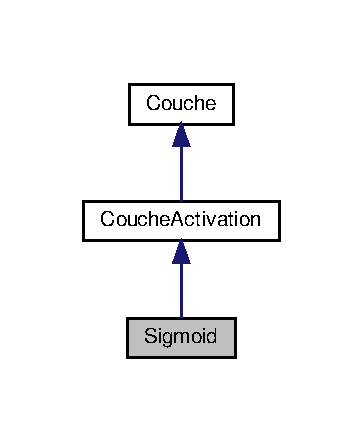
\includegraphics[width=174pt]{class_sigmoid__inherit__graph}
\end{center}
\end{figure}


Graphe de collaboration de Sigmoid\+:\nopagebreak
\begin{figure}[H]
\begin{center}
\leavevmode
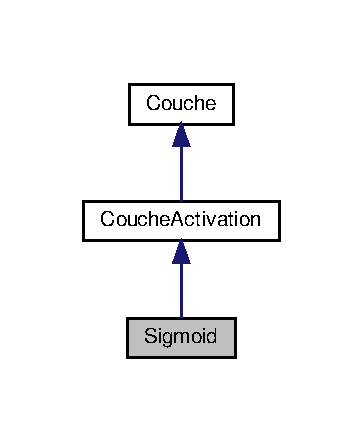
\includegraphics[width=174pt]{class_sigmoid__coll__graph}
\end{center}
\end{figure}
\subsection*{Fonctions membres publiques}
\begin{DoxyCompactItemize}
\item 
\mbox{\Hypertarget{class_sigmoid_a6085e021ce6eb13fd04b46387f4b3ccf}\label{class_sigmoid_a6085e021ce6eb13fd04b46387f4b3ccf}} 
\hyperlink{class_sigmoid_a6085e021ce6eb13fd04b46387f4b3ccf}{Sigmoid} (\hyperlink{class_dim_tenseur}{Dim\+Tenseur} din, \hyperlink{class_dim_tenseur}{Dim\+Tenseur} dout, std\+::string no)
\begin{DoxyCompactList}\small\item\em Constructeur d\textquotesingle{}une fonction sigmoid. \end{DoxyCompactList}\item 
\hyperlink{class_tenseur}{Tenseur} \hyperlink{class_sigmoid_a6bd1f6bbc49bd7e634dc33701aee420c}{propagation} (\hyperlink{class_tenseur}{Tenseur} t)
\begin{DoxyCompactList}\small\item\em Méthode permettant la propagation d\textquotesingle{}une couche à une autre. \end{DoxyCompactList}\end{DoxyCompactItemize}


\subsection{Description détaillée}
Création de la fonction \hyperlink{class_re_l_u}{Re\+LU}. 

Création d\textquotesingle{}une couche \hyperlink{class_sigmoid}{Sigmoid}.

\begin{DoxyAuthor}{Auteur}
Adrien 
\end{DoxyAuthor}
\begin{DoxyVersion}{Version}
1.\+0 
\end{DoxyVersion}
\begin{DoxyDate}{Date}
avril 2019
\end{DoxyDate}
Classe permettant la création d\textquotesingle{}une couche de type \hyperlink{class_re_l_u}{Re\+LU} (= Rectified Linear Unit). C\textquotesingle{}est à dire f(x)=max(0,x)

\begin{DoxyAuthor}{Auteur}
Adrien 
\end{DoxyAuthor}
\begin{DoxyVersion}{Version}
1.\+0 
\end{DoxyVersion}
\begin{DoxyDate}{Date}
avril 2019
\end{DoxyDate}
Classe permettant la création d\textquotesingle{}une fonction sigmoid. 

Définition à la ligne 17 du fichier Sigmoid.\+hpp.



\subsection{Documentation des fonctions membres}
\mbox{\Hypertarget{class_sigmoid_a6bd1f6bbc49bd7e634dc33701aee420c}\label{class_sigmoid_a6bd1f6bbc49bd7e634dc33701aee420c}} 
\index{Sigmoid@{Sigmoid}!propagation@{propagation}}
\index{propagation@{propagation}!Sigmoid@{Sigmoid}}
\subsubsection{\texorpdfstring{propagation()}{propagation()}}
{\footnotesize\ttfamily \hyperlink{class_tenseur}{Tenseur} Sigmoid\+::propagation (\begin{DoxyParamCaption}\item[{\hyperlink{class_tenseur}{Tenseur}}]{t }\end{DoxyParamCaption})\hspace{0.3cm}{\ttfamily [virtual]}}



Méthode permettant la propagation d\textquotesingle{}une couche à une autre. 


\begin{DoxyParams}{Paramètres}
{\em t} & le tenseur d\textquotesingle{}entree \\
\hline
\end{DoxyParams}
\begin{DoxyReturn}{Renvoie}
la sortie de la fonction sigmoid = 1./1-\/e$^\wedge$(-\/t) 
\end{DoxyReturn}


Réimplémentée à partir de \hyperlink{class_couche_a1f0ed59e21020f5d4f37933af4d1b1e5}{Couche}.



Définition à la ligne 8 du fichier Sigmoid.\+cpp.



La documentation de cette classe a été générée à partir des fichiers suivants \+:\begin{DoxyCompactItemize}
\item 
src/deeplearn/archi/Sigmoid.\+hpp\item 
src/deeplearn/archi/Sigmoid.\+cpp\end{DoxyCompactItemize}

\hypertarget{class_tan_h}{}\section{Référence de la classe TanH}
\label{class_tan_h}\index{TanH@{TanH}}


Création d\textquotesingle{}une fonction tangente hyperbolique.  




{\ttfamily \#include $<$Tan\+H.\+hpp$>$}



Graphe d\textquotesingle{}héritage de TanH\+:\nopagebreak
\begin{figure}[H]
\begin{center}
\leavevmode
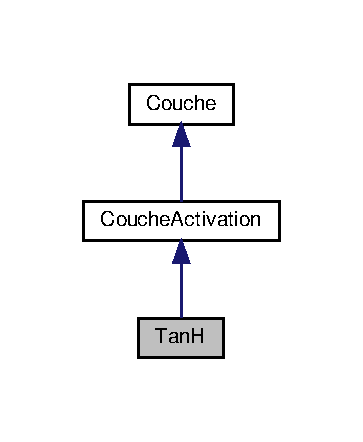
\includegraphics[width=174pt]{class_tan_h__inherit__graph}
\end{center}
\end{figure}


Graphe de collaboration de TanH\+:\nopagebreak
\begin{figure}[H]
\begin{center}
\leavevmode
\includegraphics[width=174pt]{class_tan_h__coll__graph}
\end{center}
\end{figure}
\subsection*{Fonctions membres publiques}
\begin{DoxyCompactItemize}
\item 
\mbox{\Hypertarget{class_tan_h_a15a43acf406e3ed45c632bcd451f97f6}\label{class_tan_h_a15a43acf406e3ed45c632bcd451f97f6}} 
\hyperlink{class_tan_h_a15a43acf406e3ed45c632bcd451f97f6}{TanH} (\hyperlink{class_dim_tenseur}{Dim\+Tenseur} din, \hyperlink{class_dim_tenseur}{Dim\+Tenseur} dout, std\+::string no)
\begin{DoxyCompactList}\small\item\em Constructeur d\textquotesingle{}une fonction tangente hyperbolique. \end{DoxyCompactList}\item 
\hyperlink{class_tenseur}{Tenseur} \hyperlink{class_tan_h_a869967c9b278c6592e6fcc04b61a5f0c}{propagation} (\hyperlink{class_tenseur}{Tenseur} t)
\begin{DoxyCompactList}\small\item\em Méthode permettant la propagation d\textquotesingle{}une couche à une autre. \end{DoxyCompactList}\end{DoxyCompactItemize}


\subsection{Description détaillée}
Création d\textquotesingle{}une fonction tangente hyperbolique. 

\begin{DoxyAuthor}{Auteur}
Adrien 
\end{DoxyAuthor}
\begin{DoxyVersion}{Version}
1.\+0 
\end{DoxyVersion}
\begin{DoxyDate}{Date}
avril 2019
\end{DoxyDate}
Classe permettant la création d\textquotesingle{}une fonction tangente hyperbolique Cette classe hérite de la classe \hyperlink{class_couche_activation}{Couche\+Activation}. 

Définition à la ligne 17 du fichier Tan\+H.\+hpp.



\subsection{Documentation des fonctions membres}
\mbox{\Hypertarget{class_tan_h_a869967c9b278c6592e6fcc04b61a5f0c}\label{class_tan_h_a869967c9b278c6592e6fcc04b61a5f0c}} 
\index{TanH@{TanH}!propagation@{propagation}}
\index{propagation@{propagation}!TanH@{TanH}}
\subsubsection{\texorpdfstring{propagation()}{propagation()}}
{\footnotesize\ttfamily \hyperlink{class_tenseur}{Tenseur} Tan\+H\+::propagation (\begin{DoxyParamCaption}\item[{\hyperlink{class_tenseur}{Tenseur}}]{t }\end{DoxyParamCaption})\hspace{0.3cm}{\ttfamily [virtual]}}



Méthode permettant la propagation d\textquotesingle{}une couche à une autre. 


\begin{DoxyParams}{Paramètres}
{\em t} & le tenseur d\textquotesingle{}entree \\
\hline
\end{DoxyParams}
\begin{DoxyReturn}{Renvoie}
la sortie de la fonction tanH 
\end{DoxyReturn}


Réimplémentée à partir de \hyperlink{class_couche_a1f0ed59e21020f5d4f37933af4d1b1e5}{Couche}.



Définition à la ligne 7 du fichier Tan\+H.\+cpp.



La documentation de cette classe a été générée à partir des fichiers suivants \+:\begin{DoxyCompactItemize}
\item 
src/deeplearn/archi/Tan\+H.\+hpp\item 
src/deeplearn/archi/Tan\+H.\+cpp\end{DoxyCompactItemize}

\hypertarget{class_tenseur}{}\section{Référence de la classe Tenseur}
\label{class_tenseur}\index{Tenseur@{Tenseur}}


Classe liée à la manipulation de tenseurs.  




{\ttfamily \#include $<$Tenseur.\+hpp$>$}



Graphe d\textquotesingle{}héritage de Tenseur\+:\nopagebreak
\begin{figure}[H]
\begin{center}
\leavevmode
\includegraphics[width=198pt]{class_tenseur__inherit__graph}
\end{center}
\end{figure}
\subsection*{Fonctions membres publiques}
\begin{DoxyCompactItemize}
\item 
\hyperlink{class_tenseur_a936de784ba6d02e78456091b857c90d2}{Tenseur} (int dim)
\begin{DoxyCompactList}\small\item\em Constructeur d\textquotesingle{}un tenseur dont la taille est fixée grâce à des entiers. \end{DoxyCompactList}\item 
\mbox{\Hypertarget{class_tenseur_a6a39e895e161502a104b28e108d5923e}\label{class_tenseur_a6a39e895e161502a104b28e108d5923e}} 
\hyperlink{class_tenseur_a6a39e895e161502a104b28e108d5923e}{Tenseur} (void $\ast$val, \hyperlink{class_dim_tenseur}{Dim\+Tenseur} di)
\begin{DoxyCompactList}\small\item\em Constructeur d\textquotesingle{}un tenseur dont la taille est fixée grâce à un objet \hyperlink{class_dim_tenseur}{Dim\+Tenseur}. \end{DoxyCompactList}\item 
\mbox{\Hypertarget{class_tenseur_ad8c217e97370fbe4fabe47c792f976a0}\label{class_tenseur_ad8c217e97370fbe4fabe47c792f976a0}} 
void \hyperlink{class_tenseur_ad8c217e97370fbe4fabe47c792f976a0}{init\+Valeur\+Gaussienne} ()
\begin{DoxyCompactList}\small\item\em Initialisation du tenseur selon une loi gaussienne. \end{DoxyCompactList}\item 
\mbox{\Hypertarget{class_tenseur_ad56d975cf6954e6e38116b82bc4aca3a}\label{class_tenseur_ad56d975cf6954e6e38116b82bc4aca3a}} 
void \hyperlink{class_tenseur_ad56d975cf6954e6e38116b82bc4aca3a}{init\+Valeur\+Nulle} ()
\begin{DoxyCompactList}\small\item\em Initialisation du tenseur avec des valeurs nulles. \end{DoxyCompactList}\item 
\mbox{\Hypertarget{class_tenseur_aba025d1b39fd6de6dba44b9ed4bc865a}\label{class_tenseur_aba025d1b39fd6de6dba44b9ed4bc865a}} 
void \hyperlink{class_tenseur_aba025d1b39fd6de6dba44b9ed4bc865a}{init\+Valeur\+Unif} ()
\begin{DoxyCompactList}\small\item\em Initialisation du tenseur selon une loi uniforme. \end{DoxyCompactList}\item 
void \hyperlink{class_tenseur_add5cd51caa3aae69a44dc3f0bc2b9170}{set\+Valeur} (void $\ast$vl)
\begin{DoxyCompactList}\small\item\em Méthode pour fixer la valeur du \hyperlink{class_tenseur}{Tenseur}. \end{DoxyCompactList}\item 
void \hyperlink{class_tenseur_a161be386a5d179f538234fceb152e80a}{set\+Dim} (\hyperlink{class_dim_tenseur}{Dim\+Tenseur} di)
\begin{DoxyCompactList}\small\item\em Méthode pour fixer la dimension du \hyperlink{class_tenseur}{Tenseur}. \end{DoxyCompactList}\item 
void $\ast$ \hyperlink{class_tenseur_abf24ad6abb135909d0ec82142da47188}{get\+Valeur} ()
\begin{DoxyCompactList}\small\item\em Méthode pour obtenir la valeur du \hyperlink{class_tenseur}{Tenseur}. \end{DoxyCompactList}\item 
\hyperlink{class_tenseur}{Tenseur} \hyperlink{class_tenseur_a616b8fc8cfee2c3f601c567ba42c7422}{produit\+Terme\+A\+Terme} (\hyperlink{class_tenseur}{Tenseur} t1)
\begin{DoxyCompactList}\small\item\em Méthode qui calcule le produit terme à terme entre deux tenseurs. \end{DoxyCompactList}\item 
\hyperlink{class_dim_tenseur}{Dim\+Tenseur} \hyperlink{class_tenseur_a84d2bb71deb6f4998327f6c9309c1ed4}{get\+Dim} ()
\begin{DoxyCompactList}\small\item\em Méthode pour obtenir la dimension du \hyperlink{class_tenseur}{Tenseur}. \end{DoxyCompactList}\end{DoxyCompactItemize}


\subsection{Description détaillée}
Classe liée à la manipulation de tenseurs. 

\begin{DoxyAuthor}{Auteur}
Adrien 
\end{DoxyAuthor}
\begin{DoxyVersion}{Version}
1.\+0 
\end{DoxyVersion}
\begin{DoxyDate}{Date}
avril 2019
\end{DoxyDate}
Cette classe permet de créer un tenseur de la taille souhaitée. On peut initialiser un tenseur de trois façons différentes (uniforme,nulle,gaussienne). 

Définition à la ligne 17 du fichier Tenseur.\+hpp.



\subsection{Documentation des constructeurs et destructeur}
\mbox{\Hypertarget{class_tenseur_a936de784ba6d02e78456091b857c90d2}\label{class_tenseur_a936de784ba6d02e78456091b857c90d2}} 
\index{Tenseur@{Tenseur}!Tenseur@{Tenseur}}
\index{Tenseur@{Tenseur}!Tenseur@{Tenseur}}
\subsubsection{\texorpdfstring{Tenseur()}{Tenseur()}}
{\footnotesize\ttfamily Tenseur\+::\+Tenseur (\begin{DoxyParamCaption}\item[{int}]{dim }\end{DoxyParamCaption})}



Constructeur d\textquotesingle{}un tenseur dont la taille est fixée grâce à des entiers. 


\begin{DoxyParams}{Paramètres}
{\em dim} & suite de dimensions \\
\hline
\end{DoxyParams}


\subsection{Documentation des fonctions membres}
\mbox{\Hypertarget{class_tenseur_a84d2bb71deb6f4998327f6c9309c1ed4}\label{class_tenseur_a84d2bb71deb6f4998327f6c9309c1ed4}} 
\index{Tenseur@{Tenseur}!get\+Dim@{get\+Dim}}
\index{get\+Dim@{get\+Dim}!Tenseur@{Tenseur}}
\subsubsection{\texorpdfstring{get\+Dim()}{getDim()}}
{\footnotesize\ttfamily \hyperlink{class_dim_tenseur}{Dim\+Tenseur} Tenseur\+::get\+Dim (\begin{DoxyParamCaption}{ }\end{DoxyParamCaption})}



Méthode pour obtenir la dimension du \hyperlink{class_tenseur}{Tenseur}. 

\begin{DoxyReturn}{Renvoie}
La dimension du \hyperlink{class_tenseur}{Tenseur} 
\end{DoxyReturn}


Définition à la ligne 51 du fichier Tenseur.\+cpp.

\mbox{\Hypertarget{class_tenseur_abf24ad6abb135909d0ec82142da47188}\label{class_tenseur_abf24ad6abb135909d0ec82142da47188}} 
\index{Tenseur@{Tenseur}!get\+Valeur@{get\+Valeur}}
\index{get\+Valeur@{get\+Valeur}!Tenseur@{Tenseur}}
\subsubsection{\texorpdfstring{get\+Valeur()}{getValeur()}}
{\footnotesize\ttfamily int Tenseur\+::get\+Valeur (\begin{DoxyParamCaption}{ }\end{DoxyParamCaption})}



Méthode pour obtenir la valeur du \hyperlink{class_tenseur}{Tenseur}. 

\begin{DoxyReturn}{Renvoie}
La valeur du \hyperlink{class_tenseur}{Tenseur} 
\end{DoxyReturn}


Définition à la ligne 44 du fichier Tenseur.\+cpp.

\mbox{\Hypertarget{class_tenseur_a616b8fc8cfee2c3f601c567ba42c7422}\label{class_tenseur_a616b8fc8cfee2c3f601c567ba42c7422}} 
\index{Tenseur@{Tenseur}!produit\+Terme\+A\+Terme@{produit\+Terme\+A\+Terme}}
\index{produit\+Terme\+A\+Terme@{produit\+Terme\+A\+Terme}!Tenseur@{Tenseur}}
\subsubsection{\texorpdfstring{produit\+Terme\+A\+Terme()}{produitTermeATerme()}}
{\footnotesize\ttfamily \hyperlink{class_tenseur}{Tenseur} Tenseur\+::produit\+Terme\+A\+Terme (\begin{DoxyParamCaption}\item[{\hyperlink{class_tenseur}{Tenseur}}]{t1 }\end{DoxyParamCaption})}



Méthode qui calcule le produit terme à terme entre deux tenseurs. 


\begin{DoxyParams}{Paramètres}
{\em un} & tenseur \\
\hline
\end{DoxyParams}
\begin{DoxyReturn}{Renvoie}
un tenseur 
\end{DoxyReturn}
\mbox{\Hypertarget{class_tenseur_a161be386a5d179f538234fceb152e80a}\label{class_tenseur_a161be386a5d179f538234fceb152e80a}} 
\index{Tenseur@{Tenseur}!set\+Dim@{set\+Dim}}
\index{set\+Dim@{set\+Dim}!Tenseur@{Tenseur}}
\subsubsection{\texorpdfstring{set\+Dim()}{setDim()}}
{\footnotesize\ttfamily void Tenseur\+::set\+Dim (\begin{DoxyParamCaption}\item[{\hyperlink{class_dim_tenseur}{Dim\+Tenseur}}]{di }\end{DoxyParamCaption})}



Méthode pour fixer la dimension du \hyperlink{class_tenseur}{Tenseur}. 


\begin{DoxyParams}{Paramètres}
{\em vl} & La dimension du tenseur \\
\hline
\end{DoxyParams}


Définition à la ligne 37 du fichier Tenseur.\+cpp.

\mbox{\Hypertarget{class_tenseur_add5cd51caa3aae69a44dc3f0bc2b9170}\label{class_tenseur_add5cd51caa3aae69a44dc3f0bc2b9170}} 
\index{Tenseur@{Tenseur}!set\+Valeur@{set\+Valeur}}
\index{set\+Valeur@{set\+Valeur}!Tenseur@{Tenseur}}
\subsubsection{\texorpdfstring{set\+Valeur()}{setValeur()}}
{\footnotesize\ttfamily void Tenseur\+::set\+Valeur (\begin{DoxyParamCaption}\item[{void $\ast$}]{vl }\end{DoxyParamCaption})}



Méthode pour fixer la valeur du \hyperlink{class_tenseur}{Tenseur}. 


\begin{DoxyParams}{Paramètres}
{\em vl} & La valeur du tenseur \\
\hline
\end{DoxyParams}


Définition à la ligne 30 du fichier Tenseur.\+cpp.



La documentation de cette classe a été générée à partir des fichiers suivants \+:\begin{DoxyCompactItemize}
\item 
src/deeplearn/archi/Tenseur.\+hpp\item 
src/deeplearn/archi/Tenseur.\+cpp\end{DoxyCompactItemize}

\hypertarget{class_test_couche}{}\section{Référence de la classe Test\+Couche}
\label{class_test_couche}\index{Test\+Couche@{Test\+Couche}}


Test des méthodes de la classe \hyperlink{class_couche}{Couche}.  




{\ttfamily \#include $<$Test\+Couche.\+hpp$>$}



Graphe d\textquotesingle{}héritage de Test\+Couche\+:\nopagebreak
\begin{figure}[H]
\begin{center}
\leavevmode
\includegraphics[width=272pt]{class_test_couche__inherit__graph}
\end{center}
\end{figure}


Graphe de collaboration de Test\+Couche\+:\nopagebreak
\begin{figure}[H]
\begin{center}
\leavevmode
\includegraphics[width=272pt]{class_test_couche__coll__graph}
\end{center}
\end{figure}
\subsection*{Fonctions membres publiques}
\begin{DoxyCompactItemize}
\item 
\mbox{\Hypertarget{class_test_couche_aceb4afd1f69e11bb98a0fb69c5468e85}\label{class_test_couche_aceb4afd1f69e11bb98a0fb69c5468e85}} 
void {\bfseries set\+Up} ()
\item 
\mbox{\Hypertarget{class_test_couche_a52d776a6624d1ff323b9c390be482809}\label{class_test_couche_a52d776a6624d1ff323b9c390be482809}} 
void {\bfseries tear\+Down} ()
\item 
\mbox{\Hypertarget{class_test_couche_a91abe7adddd8687482a86316995d6d2b}\label{class_test_couche_a91abe7adddd8687482a86316995d6d2b}} 
void {\bfseries test\+Get\+Dim\+Input} ()
\item 
\mbox{\Hypertarget{class_test_couche_a9f2a6f3c97c55c920acb3d552a5ccc4d}\label{class_test_couche_a9f2a6f3c97c55c920acb3d552a5ccc4d}} 
void {\bfseries test\+Get\+Dim\+Output} ()
\item 
\mbox{\Hypertarget{class_test_couche_aa192e04275717fab674f977fb24cb59e}\label{class_test_couche_aa192e04275717fab674f977fb24cb59e}} 
void {\bfseries test\+Set\+Dim\+Input} ()
\item 
\mbox{\Hypertarget{class_test_couche_a6762ad4ef2194ba9990f838d0543c851}\label{class_test_couche_a6762ad4ef2194ba9990f838d0543c851}} 
void {\bfseries test\+Set\+Dim\+Output} ()
\item 
\mbox{\Hypertarget{class_test_couche_a2012666426b127d26006dca756986575}\label{class_test_couche_a2012666426b127d26006dca756986575}} 
void {\bfseries test\+Propagation} ()
\item 
\mbox{\Hypertarget{class_test_couche_aefdfb41451d5a04fcc3e33704b900315}\label{class_test_couche_aefdfb41451d5a04fcc3e33704b900315}} 
void {\bfseries test\+Derivee} ()
\item 
\mbox{\Hypertarget{class_test_couche_aceb4afd1f69e11bb98a0fb69c5468e85}\label{class_test_couche_aceb4afd1f69e11bb98a0fb69c5468e85}} 
void \hyperlink{class_test_couche_aceb4afd1f69e11bb98a0fb69c5468e85}{set\+Up} ()
\begin{DoxyCompactList}\small\item\em Initialiser les variables. \end{DoxyCompactList}\item 
\mbox{\Hypertarget{class_test_couche_a52d776a6624d1ff323b9c390be482809}\label{class_test_couche_a52d776a6624d1ff323b9c390be482809}} 
void \hyperlink{class_test_couche_a52d776a6624d1ff323b9c390be482809}{tear\+Down} ()
\begin{DoxyCompactList}\small\item\em Supprimer les variables. \end{DoxyCompactList}\item 
\mbox{\Hypertarget{class_test_couche_a91abe7adddd8687482a86316995d6d2b}\label{class_test_couche_a91abe7adddd8687482a86316995d6d2b}} 
void \hyperlink{class_test_couche_a91abe7adddd8687482a86316995d6d2b}{test\+Get\+Dim\+Input} ()
\begin{DoxyCompactList}\small\item\em Vérifier que la propagation d\textquotesingle{}une couche à une autre se déroule normalement. \end{DoxyCompactList}\item 
\mbox{\Hypertarget{class_test_couche_a9f2a6f3c97c55c920acb3d552a5ccc4d}\label{class_test_couche_a9f2a6f3c97c55c920acb3d552a5ccc4d}} 
void {\bfseries test\+Get\+Dim\+Output} ()
\item 
\mbox{\Hypertarget{class_test_couche_aa192e04275717fab674f977fb24cb59e}\label{class_test_couche_aa192e04275717fab674f977fb24cb59e}} 
void {\bfseries test\+Set\+Dim\+Input} ()
\item 
\mbox{\Hypertarget{class_test_couche_a6762ad4ef2194ba9990f838d0543c851}\label{class_test_couche_a6762ad4ef2194ba9990f838d0543c851}} 
void {\bfseries test\+Set\+Dim\+Output} ()
\item 
\mbox{\Hypertarget{class_test_couche_a2012666426b127d26006dca756986575}\label{class_test_couche_a2012666426b127d26006dca756986575}} 
void {\bfseries test\+Propagation} ()
\item 
\mbox{\Hypertarget{class_test_couche_aefdfb41451d5a04fcc3e33704b900315}\label{class_test_couche_aefdfb41451d5a04fcc3e33704b900315}} 
void \hyperlink{class_test_couche_aefdfb41451d5a04fcc3e33704b900315}{test\+Derivee} ()
\begin{DoxyCompactList}\small\item\em Vérifier que la dérivation d\textquotesingle{}une couche s\textquotesingle{}effectue correctement. \end{DoxyCompactList}\end{DoxyCompactItemize}


\subsection{Description détaillée}
Test des méthodes de la classe \hyperlink{class_couche}{Couche}. 

\begin{DoxyAuthor}{Auteur}
Adrien 
\end{DoxyAuthor}
\begin{DoxyVersion}{Version}
1.\+0 
\end{DoxyVersion}
\begin{DoxyDate}{Date}
avril 2019 
\end{DoxyDate}


Définition à la ligne 6 du fichier Test\+Couche.\+cpp.



La documentation de cette classe a été générée à partir des fichiers suivants \+:\begin{DoxyCompactItemize}
\item 
src/deeplearn/archi/Test\+Couche.\+cpp\item 
src/deeplearn/archi/Test\+Couche.\+hpp\end{DoxyCompactItemize}

\hypertarget{class_test_donnees}{}\section{Référence de la classe Test\+Donnees}
\label{class_test_donnees}\index{Test\+Donnees@{Test\+Donnees}}


Test des méthodes de la classe \hyperlink{class_donnees}{Donnees}.  




{\ttfamily \#include $<$Test\+Donnees.\+hpp$>$}



Graphe d\textquotesingle{}héritage de Test\+Donnees\+:\nopagebreak
\begin{figure}[H]
\begin{center}
\leavevmode
\includegraphics[width=155pt]{class_test_donnees__inherit__graph}
\end{center}
\end{figure}


Graphe de collaboration de Test\+Donnees\+:\nopagebreak
\begin{figure}[H]
\begin{center}
\leavevmode
\includegraphics[width=155pt]{class_test_donnees__coll__graph}
\end{center}
\end{figure}
\subsection*{Fonctions membres publiques}
\begin{DoxyCompactItemize}
\item 
\mbox{\Hypertarget{class_test_donnees_a270d63fc0fd8310b6981225d31ccb3c5}\label{class_test_donnees_a270d63fc0fd8310b6981225d31ccb3c5}} 
void \hyperlink{class_test_donnees_a270d63fc0fd8310b6981225d31ccb3c5}{set\+Up} ()
\begin{DoxyCompactList}\small\item\em Initialiser les variables. \end{DoxyCompactList}\item 
\mbox{\Hypertarget{class_test_donnees_a19fa2b873fc882353606723ba99793c5}\label{class_test_donnees_a19fa2b873fc882353606723ba99793c5}} 
void \hyperlink{class_test_donnees_a19fa2b873fc882353606723ba99793c5}{tear\+Down} ()
\begin{DoxyCompactList}\small\item\em Supprimer les variables. \end{DoxyCompactList}\item 
\mbox{\Hypertarget{class_test_donnees_ab85dfa38fe0efc026b0c2e23b568f659}\label{class_test_donnees_ab85dfa38fe0efc026b0c2e23b568f659}} 
void \hyperlink{class_test_donnees_ab85dfa38fe0efc026b0c2e23b568f659}{test\+Ajouter\+Donnees} ()
\begin{DoxyCompactList}\small\item\em Vérifier que les données s\textquotesingle{}ajoutent bien. \end{DoxyCompactList}\item 
\mbox{\Hypertarget{class_test_donnees_a937d740393691c65aac44da6ae6a10f4}\label{class_test_donnees_a937d740393691c65aac44da6ae6a10f4}} 
void \hyperlink{class_test_donnees_a937d740393691c65aac44da6ae6a10f4}{test\+Melanger} ()
\begin{DoxyCompactList}\small\item\em Vérifier que les données se mélangent bien. \end{DoxyCompactList}\end{DoxyCompactItemize}


\subsection{Description détaillée}
Test des méthodes de la classe \hyperlink{class_donnees}{Donnees}. 

\begin{DoxyAuthor}{Auteur}
Adrien 
\end{DoxyAuthor}
\begin{DoxyVersion}{Version}
1.\+0 
\end{DoxyVersion}
\begin{DoxyDate}{Date}
avril 2019 
\end{DoxyDate}


Définition à la ligne 5 du fichier Test\+Donnees.\+cpp.



La documentation de cette classe a été générée à partir des fichiers suivants \+:\begin{DoxyCompactItemize}
\item 
src/deeplearn/train/Test\+Donnees.\+cpp\item 
src/deeplearn/train/Test\+Donnees.\+hpp\end{DoxyCompactItemize}

\hypertarget{class_test_graphe}{}\section{Référence de la classe Test\+Graphe}
\label{class_test_graphe}\index{Test\+Graphe@{Test\+Graphe}}


Test des methodes de la classe \hyperlink{class_graphe}{Graphe}.  




{\ttfamily \#include $<$Test\+Graphe.\+hpp$>$}



Graphe d\textquotesingle{}héritage de Test\+Graphe\+:\nopagebreak
\begin{figure}[H]
\begin{center}
\leavevmode
\includegraphics[width=272pt]{class_test_graphe__inherit__graph}
\end{center}
\end{figure}


Graphe de collaboration de Test\+Graphe\+:\nopagebreak
\begin{figure}[H]
\begin{center}
\leavevmode
\includegraphics[width=272pt]{class_test_graphe__coll__graph}
\end{center}
\end{figure}
\subsection*{Fonctions membres publiques}
\begin{DoxyCompactItemize}
\item 
\mbox{\Hypertarget{class_test_graphe_a45a1f586a78c1620766ff9eadf553d63}\label{class_test_graphe_a45a1f586a78c1620766ff9eadf553d63}} 
void {\bfseries set\+Up} ()
\item 
\mbox{\Hypertarget{class_test_graphe_a5fc50dc85fdc3620d6e9170cb68b4b6f}\label{class_test_graphe_a5fc50dc85fdc3620d6e9170cb68b4b6f}} 
void {\bfseries tear\+Down} ()
\item 
\mbox{\Hypertarget{class_test_graphe_a828faee28311ce705bcf8b5c450ccd09}\label{class_test_graphe_a828faee28311ce705bcf8b5c450ccd09}} 
void {\bfseries test\+Ajouter\+Noeud} ()
\item 
\mbox{\Hypertarget{class_test_graphe_aeff7e8c6e4bcf503edbb219badd66215}\label{class_test_graphe_aeff7e8c6e4bcf503edbb219badd66215}} 
void {\bfseries test\+Ajouter\+Arc} ()
\item 
\mbox{\Hypertarget{class_test_graphe_af48572064506a5bb25984156d182474e}\label{class_test_graphe_af48572064506a5bb25984156d182474e}} 
void {\bfseries test\+Supprimer\+Noeud} ()
\item 
\mbox{\Hypertarget{class_test_graphe_acec1ab448ef4822fe8071e3f204d8b0b}\label{class_test_graphe_acec1ab448ef4822fe8071e3f204d8b0b}} 
void {\bfseries test\+Supprimer\+Arc} ()
\item 
\mbox{\Hypertarget{class_test_graphe_a450232b7d114d0adef2bc0859e74b3dd}\label{class_test_graphe_a450232b7d114d0adef2bc0859e74b3dd}} 
void {\bfseries test\+Contient\+Cycle} ()
\item 
\mbox{\Hypertarget{class_test_graphe_ab45b4ccf11e1f28e94365694323c48f0}\label{class_test_graphe_ab45b4ccf11e1f28e94365694323c48f0}} 
void {\bfseries test\+Est\+Connexe} ()
\end{DoxyCompactItemize}


\subsection{Description détaillée}
Test des methodes de la classe \hyperlink{class_graphe}{Graphe}. 

\begin{DoxyAuthor}{Auteur}
Coralie 
\end{DoxyAuthor}
\begin{DoxyVersion}{Version}
1.\+0 
\end{DoxyVersion}
\begin{DoxyDate}{Date}
avril 2019 
\end{DoxyDate}


Définition à la ligne 5 du fichier Test\+Graphe.\+cpp.



La documentation de cette classe a été générée à partir des fichiers suivants \+:\begin{DoxyCompactItemize}
\item 
src/deeplearn/archi/Test\+Graphe.\+cpp\item 
src/deeplearn/archi/Test\+Graphe.\+hpp\end{DoxyCompactItemize}

\hypertarget{class_test_reseau_neurones}{}\section{Référence de la classe Test\+Reseau\+Neurones}
\label{class_test_reseau_neurones}\index{Test\+Reseau\+Neurones@{Test\+Reseau\+Neurones}}


Graphe d\textquotesingle{}héritage de Test\+Reseau\+Neurones\+:\nopagebreak
\begin{figure}[H]
\begin{center}
\leavevmode
\includegraphics[width=192pt]{class_test_reseau_neurones__inherit__graph}
\end{center}
\end{figure}


Graphe de collaboration de Test\+Reseau\+Neurones\+:\nopagebreak
\begin{figure}[H]
\begin{center}
\leavevmode
\includegraphics[width=192pt]{class_test_reseau_neurones__coll__graph}
\end{center}
\end{figure}
\subsection*{Fonctions membres publiques}
\begin{DoxyCompactItemize}
\item 
\mbox{\Hypertarget{class_test_reseau_neurones_a96258fba3363e463ae230849f4e3c236}\label{class_test_reseau_neurones_a96258fba3363e463ae230849f4e3c236}} 
void {\bfseries set\+Up} ()
\item 
\mbox{\Hypertarget{class_test_reseau_neurones_ae52666ac7cb0176354c7d3b4306deec0}\label{class_test_reseau_neurones_ae52666ac7cb0176354c7d3b4306deec0}} 
void {\bfseries tear\+Down} ()
\item 
\mbox{\Hypertarget{class_test_reseau_neurones_aaf72a0dbcbb46dbdbfb36fe61514d59d}\label{class_test_reseau_neurones_aaf72a0dbcbb46dbdbfb36fe61514d59d}} 
void {\bfseries test\+Get\+Couche\+Initiale} ()
\item 
\mbox{\Hypertarget{class_test_reseau_neurones_a9808a8c9c28f167845db1e6f57435bb3}\label{class_test_reseau_neurones_a9808a8c9c28f167845db1e6f57435bb3}} 
void {\bfseries test\+Get\+Couche\+Finale} ()
\item 
\mbox{\Hypertarget{class_test_reseau_neurones_a2aa4cdb205ead6f6275db97894c1be09}\label{class_test_reseau_neurones_a2aa4cdb205ead6f6275db97894c1be09}} 
void {\bfseries test\+Ajouter\+Couche\+Initiale} ()
\item 
\mbox{\Hypertarget{class_test_reseau_neurones_a2cc008d42aff3d270ae3e1f935fbf6b8}\label{class_test_reseau_neurones_a2cc008d42aff3d270ae3e1f935fbf6b8}} 
void {\bfseries test\+Ajouter\+Couche\+Finale} ()
\item 
\mbox{\Hypertarget{class_test_reseau_neurones_a289a476c4f62458cb9ded841ea1b4148}\label{class_test_reseau_neurones_a289a476c4f62458cb9ded841ea1b4148}} 
void {\bfseries test\+Supprimer\+Couche\+Initiale} ()
\item 
\mbox{\Hypertarget{class_test_reseau_neurones_a0e733607d7e5bbd48a3d6e5b62d5991f}\label{class_test_reseau_neurones_a0e733607d7e5bbd48a3d6e5b62d5991f}} 
void {\bfseries test\+Supprimer\+Couche\+Finale} ()
\item 
\mbox{\Hypertarget{class_test_reseau_neurones_a96258fba3363e463ae230849f4e3c236}\label{class_test_reseau_neurones_a96258fba3363e463ae230849f4e3c236}} 
void {\bfseries set\+Up} ()
\item 
\mbox{\Hypertarget{class_test_reseau_neurones_ae52666ac7cb0176354c7d3b4306deec0}\label{class_test_reseau_neurones_ae52666ac7cb0176354c7d3b4306deec0}} 
void {\bfseries tear\+Down} ()
\item 
\mbox{\Hypertarget{class_test_reseau_neurones_aaf72a0dbcbb46dbdbfb36fe61514d59d}\label{class_test_reseau_neurones_aaf72a0dbcbb46dbdbfb36fe61514d59d}} 
void {\bfseries test\+Get\+Couche\+Initiale} ()
\item 
\mbox{\Hypertarget{class_test_reseau_neurones_a9808a8c9c28f167845db1e6f57435bb3}\label{class_test_reseau_neurones_a9808a8c9c28f167845db1e6f57435bb3}} 
void {\bfseries test\+Get\+Couche\+Finale} ()
\item 
\mbox{\Hypertarget{class_test_reseau_neurones_a2aa4cdb205ead6f6275db97894c1be09}\label{class_test_reseau_neurones_a2aa4cdb205ead6f6275db97894c1be09}} 
void {\bfseries test\+Ajouter\+Couche\+Initiale} ()
\item 
\mbox{\Hypertarget{class_test_reseau_neurones_a2cc008d42aff3d270ae3e1f935fbf6b8}\label{class_test_reseau_neurones_a2cc008d42aff3d270ae3e1f935fbf6b8}} 
void {\bfseries test\+Ajouter\+Couche\+Finale} ()
\item 
\mbox{\Hypertarget{class_test_reseau_neurones_a289a476c4f62458cb9ded841ea1b4148}\label{class_test_reseau_neurones_a289a476c4f62458cb9ded841ea1b4148}} 
void {\bfseries test\+Supprimer\+Couche\+Initiale} ()
\item 
\mbox{\Hypertarget{class_test_reseau_neurones_a0e733607d7e5bbd48a3d6e5b62d5991f}\label{class_test_reseau_neurones_a0e733607d7e5bbd48a3d6e5b62d5991f}} 
void {\bfseries test\+Supprimer\+Couche\+Finale} ()
\end{DoxyCompactItemize}


\subsection{Description détaillée}


Définition à la ligne 6 du fichier Test\+Reseau\+Neurones.\+cpp.



La documentation de cette classe a été générée à partir des fichiers suivants \+:\begin{DoxyCompactItemize}
\item 
src/deeplearn/archi/Test\+Reseau\+Neurones.\+cpp\item 
src/deeplearn/archi/Test\+Reseau\+Neurones.\+hpp\end{DoxyCompactItemize}

\hypertarget{class_test_tenseur}{}\section{Référence de la classe Test\+Tenseur}
\label{class_test_tenseur}\index{Test\+Tenseur@{Test\+Tenseur}}


Graphe d\textquotesingle{}héritage de Test\+Tenseur\+:\nopagebreak
\begin{figure}[H]
\begin{center}
\leavevmode
\includegraphics[width=151pt]{class_test_tenseur__inherit__graph}
\end{center}
\end{figure}


Graphe de collaboration de Test\+Tenseur\+:\nopagebreak
\begin{figure}[H]
\begin{center}
\leavevmode
\includegraphics[width=151pt]{class_test_tenseur__coll__graph}
\end{center}
\end{figure}
\subsection*{Fonctions membres publiques}
\begin{DoxyCompactItemize}
\item 
\mbox{\Hypertarget{class_test_tenseur_a52db9b85a9aea7ae91c5f4d6f7ca2615}\label{class_test_tenseur_a52db9b85a9aea7ae91c5f4d6f7ca2615}} 
void {\bfseries set\+Up} ()
\item 
\mbox{\Hypertarget{class_test_tenseur_afd5cb5d1ff64bc398e8d18ac9eaa00c9}\label{class_test_tenseur_afd5cb5d1ff64bc398e8d18ac9eaa00c9}} 
void {\bfseries tear\+Down} ()
\item 
\mbox{\Hypertarget{class_test_tenseur_a8bf3e16120293a440787b7094894fd6e}\label{class_test_tenseur_a8bf3e16120293a440787b7094894fd6e}} 
void {\bfseries test\+Get\+Valeur} ()
\item 
\mbox{\Hypertarget{class_test_tenseur_a771d6bd087d586718600b270bd9c51f0}\label{class_test_tenseur_a771d6bd087d586718600b270bd9c51f0}} 
void {\bfseries test\+Init\+Valeur\+Gaussienne} ()
\item 
\mbox{\Hypertarget{class_test_tenseur_a8daa25d92350bec7717fb97cd8c4868c}\label{class_test_tenseur_a8daa25d92350bec7717fb97cd8c4868c}} 
void {\bfseries test\+Init\+Valeur\+Unif} (int valeur)
\item 
\mbox{\Hypertarget{class_test_tenseur_a9ed1780c80804210fb84e7d2f3213d05}\label{class_test_tenseur_a9ed1780c80804210fb84e7d2f3213d05}} 
void {\bfseries test\+Init\+Valeur\+Nulle} ()
\item 
\mbox{\Hypertarget{class_test_tenseur_a52db9b85a9aea7ae91c5f4d6f7ca2615}\label{class_test_tenseur_a52db9b85a9aea7ae91c5f4d6f7ca2615}} 
void {\bfseries set\+Up} ()
\item 
\mbox{\Hypertarget{class_test_tenseur_afd5cb5d1ff64bc398e8d18ac9eaa00c9}\label{class_test_tenseur_afd5cb5d1ff64bc398e8d18ac9eaa00c9}} 
void {\bfseries tear\+Down} ()
\item 
\mbox{\Hypertarget{class_test_tenseur_a8bf3e16120293a440787b7094894fd6e}\label{class_test_tenseur_a8bf3e16120293a440787b7094894fd6e}} 
void {\bfseries test\+Get\+Valeur} ()
\item 
\mbox{\Hypertarget{class_test_tenseur_a771d6bd087d586718600b270bd9c51f0}\label{class_test_tenseur_a771d6bd087d586718600b270bd9c51f0}} 
void {\bfseries test\+Init\+Valeur\+Gaussienne} ()
\item 
\mbox{\Hypertarget{class_test_tenseur_a8daa25d92350bec7717fb97cd8c4868c}\label{class_test_tenseur_a8daa25d92350bec7717fb97cd8c4868c}} 
void {\bfseries test\+Init\+Valeur\+Unif} (int valeur)
\item 
\mbox{\Hypertarget{class_test_tenseur_a9ed1780c80804210fb84e7d2f3213d05}\label{class_test_tenseur_a9ed1780c80804210fb84e7d2f3213d05}} 
void {\bfseries test\+Init\+Valeur\+Nulle} ()
\end{DoxyCompactItemize}


\subsection{Description détaillée}


Définition à la ligne 6 du fichier Test\+Tenseur.\+cpp.



La documentation de cette classe a été générée à partir des fichiers suivants \+:\begin{DoxyCompactItemize}
\item 
src/deeplearn/archi/Test\+Tenseur.\+cpp\item 
src/deeplearn/archi/Test\+Tenseur.\+hpp\end{DoxyCompactItemize}

\hypertarget{class_vecteur}{}\section{Référence de la classe Vecteur}
\label{class_vecteur}\index{Vecteur@{Vecteur}}


Classe qui crée un vecteur.  




{\ttfamily \#include $<$Vecteur.\+hpp$>$}



Graphe d\textquotesingle{}héritage de Vecteur\+:\nopagebreak
\begin{figure}[H]
\begin{center}
\leavevmode
\includegraphics[width=132pt]{class_vecteur__inherit__graph}
\end{center}
\end{figure}


Graphe de collaboration de Vecteur\+:\nopagebreak
\begin{figure}[H]
\begin{center}
\leavevmode
\includegraphics[width=132pt]{class_vecteur__coll__graph}
\end{center}
\end{figure}
\subsection*{Fonctions membres publiques}
\begin{DoxyCompactItemize}
\item 
\mbox{\Hypertarget{class_vecteur_a71bd85d7378f24e08e9507570d822b7e}\label{class_vecteur_a71bd85d7378f24e08e9507570d822b7e}} 
\hyperlink{class_vecteur_a71bd85d7378f24e08e9507570d822b7e}{Vecteur} (void $\ast$vl, int l)
\begin{DoxyCompactList}\small\item\em Constructeur d\textquotesingle{}un vecteur de longueur l. \end{DoxyCompactList}\item 
double \hyperlink{class_vecteur_a21c930ceae6b18def6b37689abceeef7}{produit\+Scalaire} (\hyperlink{class_vecteur}{Vecteur} v1)
\begin{DoxyCompactList}\small\item\em Méthode qui calcule le produit scalaire entre 2 vecteurs. \end{DoxyCompactList}\end{DoxyCompactItemize}


\subsection{Description détaillée}
Classe qui crée un vecteur. 

\begin{DoxyAuthor}{Auteur}
Adrien 
\end{DoxyAuthor}
\begin{DoxyVersion}{Version}
1.\+0 
\end{DoxyVersion}
\begin{DoxyDate}{Date}
avril 2019
\end{DoxyDate}
Classe qui crée un tenseur d\textquotesingle{}ordre 1 (= vecteur) 

Définition à la ligne 17 du fichier Vecteur.\+hpp.



\subsection{Documentation des fonctions membres}
\mbox{\Hypertarget{class_vecteur_a21c930ceae6b18def6b37689abceeef7}\label{class_vecteur_a21c930ceae6b18def6b37689abceeef7}} 
\index{Vecteur@{Vecteur}!produit\+Scalaire@{produit\+Scalaire}}
\index{produit\+Scalaire@{produit\+Scalaire}!Vecteur@{Vecteur}}
\subsubsection{\texorpdfstring{produit\+Scalaire()}{produitScalaire()}}
{\footnotesize\ttfamily double Vecteur\+::produit\+Scalaire (\begin{DoxyParamCaption}\item[{\hyperlink{class_vecteur}{Vecteur}}]{v1 }\end{DoxyParamCaption})}



Méthode qui calcule le produit scalaire entre 2 vecteurs. 


\begin{DoxyParams}{Paramètres}
{\em un} & vecteur \\
\hline
\end{DoxyParams}
\begin{DoxyReturn}{Renvoie}
un réel 
\end{DoxyReturn}


La documentation de cette classe a été générée à partir des fichiers suivants \+:\begin{DoxyCompactItemize}
\item 
src/deeplearn/archi/Vecteur.\+hpp\item 
src/deeplearn/archi/Vecteur.\+cpp\end{DoxyCompactItemize}

%--- End generated contents ---

% Index
\backmatter
\newpage
\phantomsection
\clearemptydoublepage
\addcontentsline{toc}{chapter}{Index}
\printindex

\end{document}
